% auto-extracted figures from chapter1_annotated.tex (names: figXa, figXb, ...)

\newcommand{\figXa}{%
\begin{tikzpicture}[scale=0.5,line join=round]
  \draw[thick] (0,0)--(3,0)--(3,3)--(0,3)--cycle; \draw[thick] (3,0)--(4.3,1.3)--(4.3,4.3)--(3,3); \draw[thick] (0,3)--(1.3,4.3)--(4.3,4.3);
  \draw[thick,dashed,gray] (0,0)--(1.3,1.3)--(4.3,1.3); \draw[thick,dashed,gray] (1.3,1.3)--(1.3,4.3);
  \draw[very thick,mkc] (2.15,-0.6)--(2.15,4.9);
  \draw[very thick,mkc] (-0.5,2.15)--(4.8,2.15);
  \draw[very thick,mkc] (0.9,0.9)--(3.4,3.4);
  \node[font=\small\bfseries] at (2.15,-1.0) {3 face axes};
  \node[font=\scriptsize,align=center,text width=6.4cm] at (2.15,-2.1) {top--bottom, left--right, front--back; each joins the centres of two opposite faces. Three turns about each: $3\cdot3=9$ turns.};
\end{tikzpicture}}

\newcommand{\figXb}{%
\begin{tikzpicture}[scale=0.58,line join=round]
\begin{scope}[shift={(0,0)}]
  \draw[thick] (0,0)--(3,0)--(3,3)--(0,3)--cycle; \draw[thick] (3,0)--(4.3,1.3)--(4.3,4.3)--(3,3); \draw[thick] (0,3)--(1.3,4.3)--(4.3,4.3);
  \draw[thick,dashed,gray] (0,0)--(1.3,1.3)--(4.3,1.3); \draw[thick,dashed,gray] (1.3,1.3)--(1.3,4.3);
  \draw[very thick,mkc] (2.15,-0.7)--(2.15,5.1);
  \draw[-{Stealth[length=4pt]},mkc,thick] (3.15,3.65) arc (0:300:1.0 and 0.35);
  \node[font=\scriptsize\bfseries,circle,inner sep=1pt,minimum size=11pt,fill=red!80!black!30,draw=red!80!black,thick,text=black] at (0,0) {$A$};
  \node[font=\scriptsize\bfseries,circle,inner sep=1pt,minimum size=11pt,fill=orange!95!black!30,draw=orange!95!black,thick,text=black] at (3,0) {$B$};
  \node[font=\scriptsize\bfseries,circle,inner sep=1pt,minimum size=11pt,fill=green!60!black!30,draw=green!60!black,thick,text=black] at (3,3) {$C$};
  \node[font=\scriptsize\bfseries,circle,inner sep=1pt,minimum size=11pt,fill=blue!70!black!30,draw=blue!70!black,thick,text=black] at (0,3) {$D$};
  \node[font=\scriptsize\bfseries,circle,inner sep=1pt,minimum size=11pt,fill=violet!30,draw=violet,thick,text=black] at (1.3,1.3) {$E$};
  \node[font=\scriptsize\bfseries,circle,inner sep=1pt,minimum size=11pt,fill=cyan!65!black!30,draw=cyan!65!black,thick,text=black] at (4.3,1.3) {$F$};
  \node[font=\scriptsize\bfseries,circle,inner sep=1pt,minimum size=11pt,fill=brown!80!black!30,draw=brown!80!black,thick,text=black] at (4.3,4.3) {$G$};
  \node[font=\scriptsize\bfseries,circle,inner sep=1pt,minimum size=11pt,fill=magenta!75!black!30,draw=magenta!75!black,thick,text=black] at (1.3,4.3) {$H$};
\end{scope}
  \draw[-{Stealth[length=5pt]},very thick,mkc] (5.4,2.15) -- node[above,font=\scriptsize,mkc,align=center] {quarter turn\\$90^\circ$} (7.0,2.15);
\begin{scope}[shift={(7.6,0)}]
  \draw[thick] (0,0)--(3,0)--(3,3)--(0,3)--cycle; \draw[thick] (3,0)--(4.3,1.3)--(4.3,4.3)--(3,3); \draw[thick] (0,3)--(1.3,4.3)--(4.3,4.3);
  \draw[thick,dashed,gray] (0,0)--(1.3,1.3)--(4.3,1.3); \draw[thick,dashed,gray] (1.3,1.3)--(1.3,4.3);
  \draw[very thick,mkc] (2.15,-0.7)--(2.15,5.1);
  \node[font=\scriptsize\bfseries,circle,inner sep=1pt,minimum size=11pt,fill=red!80!black!30,draw=red!80!black,thick,text=black] at (3,0) {$A$};
  \node[font=\scriptsize\bfseries,circle,inner sep=1pt,minimum size=11pt,fill=orange!95!black!30,draw=orange!95!black,thick,text=black] at (4.3,1.3) {$B$};
  \node[font=\scriptsize\bfseries,circle,inner sep=1pt,minimum size=11pt,fill=cyan!65!black!30,draw=cyan!65!black,thick,text=black] at (1.3,1.3) {$F$};
  \node[font=\scriptsize\bfseries,circle,inner sep=1pt,minimum size=11pt,fill=violet!30,draw=violet,thick,text=black] at (0,0) {$E$};
  \node[font=\scriptsize\bfseries,circle,inner sep=1pt,minimum size=11pt,fill=blue!70!black!30,draw=blue!70!black,thick,text=black] at (3,3) {$D$};
  \node[font=\scriptsize\bfseries,circle,inner sep=1pt,minimum size=11pt,fill=green!60!black!30,draw=green!60!black,thick,text=black] at (4.3,4.3) {$C$};
  \node[font=\scriptsize\bfseries,circle,inner sep=1pt,minimum size=11pt,fill=brown!80!black!30,draw=brown!80!black,thick,text=black] at (1.3,4.3) {$G$};
  \node[font=\scriptsize\bfseries,circle,inner sep=1pt,minimum size=11pt,fill=magenta!75!black!30,draw=magenta!75!black,thick,text=black] at (0,3) {$H$};
\end{scope}
  \node[font=\scriptsize,anchor=north west] at (-0.6,-0.7) {before};
  \node[font=\scriptsize,anchor=north west] at (7.0,-0.7) {after};
\begin{scope}[shift={(15.6,2.15)}]
  \draw[thick] (-1.55,-1.55) rectangle (1.55,1.55);
  \fill[mkc] (0,0) circle (2.2pt);
  \draw[-{Stealth[length=4pt]},mkc,thick] (0.85,0) arc (0:290:0.85);
  \node[font=\scriptsize\bfseries,circle,inner sep=1pt,minimum size=11pt,fill=blue!70!black!30,draw=blue!70!black,thick,text=black] at (-1.55,-1.55) {$D$};
  \node[font=\scriptsize\bfseries,circle,inner sep=1pt,minimum size=11pt,fill=green!60!black!30,draw=green!60!black,thick,text=black] at (1.55,-1.55) {$C$};
  \node[font=\scriptsize\bfseries,circle,inner sep=1pt,minimum size=11pt,fill=brown!80!black!30,draw=brown!80!black,thick,text=black] at (1.55,1.55) {$G$};
  \node[font=\scriptsize\bfseries,circle,inner sep=1pt,minimum size=11pt,fill=magenta!75!black!30,draw=magenta!75!black,thick,text=black] at (-1.55,1.55) {$H$};
\end{scope}
  \draw[-{Stealth[length=5pt]},very thick,mkc] (18.2,2.15) -- (19.6,2.15);
\begin{scope}[shift={(22.2,2.15)}]
  \draw[thick] (-1.55,-1.55) rectangle (1.55,1.55);
  \fill[mkc] (0,0) circle (2.2pt);
  \node[font=\scriptsize\bfseries,circle,inner sep=1pt,minimum size=11pt,fill=magenta!75!black!30,draw=magenta!75!black,thick,text=black] at (-1.55,-1.55) {$H$};
  \node[font=\scriptsize\bfseries,circle,inner sep=1pt,minimum size=11pt,fill=blue!70!black!30,draw=blue!70!black,thick,text=black] at (1.55,-1.55) {$D$};
  \node[font=\scriptsize\bfseries,circle,inner sep=1pt,minimum size=11pt,fill=green!60!black!30,draw=green!60!black,thick,text=black] at (1.55,1.55) {$C$};
  \node[font=\scriptsize\bfseries,circle,inner sep=1pt,minimum size=11pt,fill=brown!80!black!30,draw=brown!80!black,thick,text=black] at (-1.55,1.55) {$G$};
\end{scope}
  \node[font=\scriptsize,anchor=north] at (18.9,-0.7) {top view, looking down the axis: before $\to$ after};
  \node[font=\scriptsize,align=left,text width=8.6cm,anchor=north west] at (25.2,4.9) {\textbf{Quarter turn, $90^\circ$.} Each corner of the bottom face moves one place round, $A\to B\to F\to E\to A$, and so does the top face, $D\to C\to G\to H\to D$. Diagonals: $d_1\to d_2\to d_4\to d_3\to d_1$, a 4-cycle. \emph{Top view} down the face axis, from above the top face: the square $DCGH$; $A,B,F,E$ are hidden beneath $D,C,G,H$, and the axis is the orange dot at the centre. The ring of four colours steps round by one quarter.};
\begin{scope}[shift={(0,-8.6)}]
  \draw[thick] (0,0)--(3,0)--(3,3)--(0,3)--cycle; \draw[thick] (3,0)--(4.3,1.3)--(4.3,4.3)--(3,3); \draw[thick] (0,3)--(1.3,4.3)--(4.3,4.3);
  \draw[thick,dashed,gray] (0,0)--(1.3,1.3)--(4.3,1.3); \draw[thick,dashed,gray] (1.3,1.3)--(1.3,4.3);
  \draw[very thick,mkc] (2.15,-0.7)--(2.15,5.1);
  \draw[-{Stealth[length=4pt]},mkc,thick] (3.15,3.65) arc (0:170:1.0 and 0.35);
  \node[font=\scriptsize\bfseries,circle,inner sep=1pt,minimum size=11pt,fill=red!80!black!30,draw=red!80!black,thick,text=black] at (0,0) {$A$};
  \node[font=\scriptsize\bfseries,circle,inner sep=1pt,minimum size=11pt,fill=orange!95!black!30,draw=orange!95!black,thick,text=black] at (3,0) {$B$};
  \node[font=\scriptsize\bfseries,circle,inner sep=1pt,minimum size=11pt,fill=green!60!black!30,draw=green!60!black,thick,text=black] at (3,3) {$C$};
  \node[font=\scriptsize\bfseries,circle,inner sep=1pt,minimum size=11pt,fill=blue!70!black!30,draw=blue!70!black,thick,text=black] at (0,3) {$D$};
  \node[font=\scriptsize\bfseries,circle,inner sep=1pt,minimum size=11pt,fill=violet!30,draw=violet,thick,text=black] at (1.3,1.3) {$E$};
  \node[font=\scriptsize\bfseries,circle,inner sep=1pt,minimum size=11pt,fill=cyan!65!black!30,draw=cyan!65!black,thick,text=black] at (4.3,1.3) {$F$};
  \node[font=\scriptsize\bfseries,circle,inner sep=1pt,minimum size=11pt,fill=brown!80!black!30,draw=brown!80!black,thick,text=black] at (4.3,4.3) {$G$};
  \node[font=\scriptsize\bfseries,circle,inner sep=1pt,minimum size=11pt,fill=magenta!75!black!30,draw=magenta!75!black,thick,text=black] at (1.3,4.3) {$H$};
\end{scope}
  \draw[-{Stealth[length=5pt]},very thick,mkc] (5.4,-6.45) -- node[above,font=\scriptsize,mkc,align=center] {half turn\\$180^\circ$} (7.0,-6.45);
\begin{scope}[shift={(7.6,-8.6)}]
  \draw[thick] (0,0)--(3,0)--(3,3)--(0,3)--cycle; \draw[thick] (3,0)--(4.3,1.3)--(4.3,4.3)--(3,3); \draw[thick] (0,3)--(1.3,4.3)--(4.3,4.3);
  \draw[thick,dashed,gray] (0,0)--(1.3,1.3)--(4.3,1.3); \draw[thick,dashed,gray] (1.3,1.3)--(1.3,4.3);
  \draw[very thick,mkc] (2.15,-0.7)--(2.15,5.1);
  \node[font=\scriptsize\bfseries,circle,inner sep=1pt,minimum size=11pt,fill=red!80!black!30,draw=red!80!black,thick,text=black] at (4.3,1.3) {$A$};
  \node[font=\scriptsize\bfseries,circle,inner sep=1pt,minimum size=11pt,fill=cyan!65!black!30,draw=cyan!65!black,thick,text=black] at (0,0) {$F$};
  \node[font=\scriptsize\bfseries,circle,inner sep=1pt,minimum size=11pt,fill=orange!95!black!30,draw=orange!95!black,thick,text=black] at (1.3,1.3) {$B$};
  \node[font=\scriptsize\bfseries,circle,inner sep=1pt,minimum size=11pt,fill=violet!30,draw=violet,thick,text=black] at (3,0) {$E$};
  \node[font=\scriptsize\bfseries,circle,inner sep=1pt,minimum size=11pt,fill=green!60!black!30,draw=green!60!black,thick,text=black] at (1.3,4.3) {$C$};
  \node[font=\scriptsize\bfseries,circle,inner sep=1pt,minimum size=11pt,fill=magenta!75!black!30,draw=magenta!75!black,thick,text=black] at (3,3) {$H$};
  \node[font=\scriptsize\bfseries,circle,inner sep=1pt,minimum size=11pt,fill=blue!70!black!30,draw=blue!70!black,thick,text=black] at (4.3,4.3) {$D$};
  \node[font=\scriptsize\bfseries,circle,inner sep=1pt,minimum size=11pt,fill=brown!80!black!30,draw=brown!80!black,thick,text=black] at (0,3) {$G$};
\end{scope}
  \node[font=\scriptsize,anchor=north west] at (-0.6,-9.3) {before};
  \node[font=\scriptsize,anchor=north west] at (7.0,-9.3) {after};
\begin{scope}[shift={(15.6,-6.45)}]
  \draw[thick] (-1.55,-1.55) rectangle (1.55,1.55);
  \fill[mkc] (0,0) circle (2.2pt);
  \draw[-{Stealth[length=4pt]},mkc,thick] (0.85,0) arc (0:170:0.85);
  \node[font=\scriptsize\bfseries,circle,inner sep=1pt,minimum size=11pt,fill=blue!70!black!30,draw=blue!70!black,thick,text=black] at (-1.55,-1.55) {$D$};
  \node[font=\scriptsize\bfseries,circle,inner sep=1pt,minimum size=11pt,fill=green!60!black!30,draw=green!60!black,thick,text=black] at (1.55,-1.55) {$C$};
  \node[font=\scriptsize\bfseries,circle,inner sep=1pt,minimum size=11pt,fill=brown!80!black!30,draw=brown!80!black,thick,text=black] at (1.55,1.55) {$G$};
  \node[font=\scriptsize\bfseries,circle,inner sep=1pt,minimum size=11pt,fill=magenta!75!black!30,draw=magenta!75!black,thick,text=black] at (-1.55,1.55) {$H$};
\end{scope}
  \draw[-{Stealth[length=5pt]},very thick,mkc] (18.2,-6.45) -- (19.6,-6.45);
\begin{scope}[shift={(22.2,-6.45)}]
  \draw[thick] (-1.55,-1.55) rectangle (1.55,1.55);
  \fill[mkc] (0,0) circle (2.2pt);
  \node[font=\scriptsize\bfseries,circle,inner sep=1pt,minimum size=11pt,fill=brown!80!black!30,draw=brown!80!black,thick,text=black] at (-1.55,-1.55) {$G$};
  \node[font=\scriptsize\bfseries,circle,inner sep=1pt,minimum size=11pt,fill=magenta!75!black!30,draw=magenta!75!black,thick,text=black] at (1.55,-1.55) {$H$};
  \node[font=\scriptsize\bfseries,circle,inner sep=1pt,minimum size=11pt,fill=blue!70!black!30,draw=blue!70!black,thick,text=black] at (1.55,1.55) {$D$};
  \node[font=\scriptsize\bfseries,circle,inner sep=1pt,minimum size=11pt,fill=green!60!black!30,draw=green!60!black,thick,text=black] at (-1.55,1.55) {$C$};
\end{scope}
  \node[font=\scriptsize,anchor=north] at (18.9,-9.3) {top view, looking down the axis: before $\to$ after};
  \node[font=\scriptsize,align=left,text width=8.6cm,anchor=north west] at (25.2,-3.7) {\textbf{Half turn, $180^\circ$.} Every corner jumps to the opposite corner of its face: $A\leftrightarrow F$, $B\leftrightarrow E$, $C\leftrightarrow H$, $D\leftrightarrow G$. Diagonals: $(d_1\,d_4)(d_2\,d_3)$, two disjoint swaps. \emph{Top view} down the face axis, from above the top face: the square $DCGH$; $A,B,F,E$ are hidden beneath $D,C,G,H$, and the axis is the orange dot at the centre. Each colour goes to the diametrically opposite corner of the square.};
\begin{scope}[shift={(0,-17.2)}]
  \draw[thick] (0,0)--(3,0)--(3,3)--(0,3)--cycle; \draw[thick] (3,0)--(4.3,1.3)--(4.3,4.3)--(3,3); \draw[thick] (0,3)--(1.3,4.3)--(4.3,4.3);
  \draw[thick,dashed,gray] (0,0)--(1.3,1.3)--(4.3,1.3); \draw[thick,dashed,gray] (1.3,1.3)--(1.3,4.3);
  \draw[very thick,mkc] (2.15,-0.7)--(2.15,5.1);
  \draw[-{Stealth[length=4pt]},mkc,thick] (1.15,3.65) arc (180:-120:1.0 and 0.35);
  \node[font=\scriptsize\bfseries,circle,inner sep=1pt,minimum size=11pt,fill=red!80!black!30,draw=red!80!black,thick,text=black] at (0,0) {$A$};
  \node[font=\scriptsize\bfseries,circle,inner sep=1pt,minimum size=11pt,fill=orange!95!black!30,draw=orange!95!black,thick,text=black] at (3,0) {$B$};
  \node[font=\scriptsize\bfseries,circle,inner sep=1pt,minimum size=11pt,fill=green!60!black!30,draw=green!60!black,thick,text=black] at (3,3) {$C$};
  \node[font=\scriptsize\bfseries,circle,inner sep=1pt,minimum size=11pt,fill=blue!70!black!30,draw=blue!70!black,thick,text=black] at (0,3) {$D$};
  \node[font=\scriptsize\bfseries,circle,inner sep=1pt,minimum size=11pt,fill=violet!30,draw=violet,thick,text=black] at (1.3,1.3) {$E$};
  \node[font=\scriptsize\bfseries,circle,inner sep=1pt,minimum size=11pt,fill=cyan!65!black!30,draw=cyan!65!black,thick,text=black] at (4.3,1.3) {$F$};
  \node[font=\scriptsize\bfseries,circle,inner sep=1pt,minimum size=11pt,fill=brown!80!black!30,draw=brown!80!black,thick,text=black] at (4.3,4.3) {$G$};
  \node[font=\scriptsize\bfseries,circle,inner sep=1pt,minimum size=11pt,fill=magenta!75!black!30,draw=magenta!75!black,thick,text=black] at (1.3,4.3) {$H$};
\end{scope}
  \draw[-{Stealth[length=5pt]},very thick,mkc] (5.4,-15.05) -- node[above,font=\scriptsize,mkc,align=center] {three-quarter\\turn $270^\circ$} (7.0,-15.05);
\begin{scope}[shift={(7.6,-17.2)}]
  \draw[thick] (0,0)--(3,0)--(3,3)--(0,3)--cycle; \draw[thick] (3,0)--(4.3,1.3)--(4.3,4.3)--(3,3); \draw[thick] (0,3)--(1.3,4.3)--(4.3,4.3);
  \draw[thick,dashed,gray] (0,0)--(1.3,1.3)--(4.3,1.3); \draw[thick,dashed,gray] (1.3,1.3)--(1.3,4.3);
  \draw[very thick,mkc] (2.15,-0.7)--(2.15,5.1);
  \node[font=\scriptsize\bfseries,circle,inner sep=1pt,minimum size=11pt,fill=orange!95!black!30,draw=orange!95!black,thick,text=black] at (0,0) {$B$};
  \node[font=\scriptsize\bfseries,circle,inner sep=1pt,minimum size=11pt,fill=cyan!65!black!30,draw=cyan!65!black,thick,text=black] at (3,0) {$F$};
  \node[font=\scriptsize\bfseries,circle,inner sep=1pt,minimum size=11pt,fill=violet!30,draw=violet,thick,text=black] at (4.3,1.3) {$E$};
  \node[font=\scriptsize\bfseries,circle,inner sep=1pt,minimum size=11pt,fill=red!80!black!30,draw=red!80!black,thick,text=black] at (1.3,1.3) {$A$};
  \node[font=\scriptsize\bfseries,circle,inner sep=1pt,minimum size=11pt,fill=green!60!black!30,draw=green!60!black,thick,text=black] at (0,3) {$C$};
  \node[font=\scriptsize\bfseries,circle,inner sep=1pt,minimum size=11pt,fill=brown!80!black!30,draw=brown!80!black,thick,text=black] at (3,3) {$G$};
  \node[font=\scriptsize\bfseries,circle,inner sep=1pt,minimum size=11pt,fill=magenta!75!black!30,draw=magenta!75!black,thick,text=black] at (4.3,4.3) {$H$};
  \node[font=\scriptsize\bfseries,circle,inner sep=1pt,minimum size=11pt,fill=blue!70!black!30,draw=blue!70!black,thick,text=black] at (1.3,4.3) {$D$};
\end{scope}
  \node[font=\scriptsize,anchor=north west] at (-0.6,-17.9) {before};
  \node[font=\scriptsize,anchor=north west] at (7.0,-17.9) {after};
\begin{scope}[shift={(15.6,-15.05)}]
  \draw[thick] (-1.55,-1.55) rectangle (1.55,1.55);
  \fill[mkc] (0,0) circle (2.2pt);
  \draw[-{Stealth[length=4pt]},mkc,thick] (-0.85,0) arc (180:-110:0.85);
  \node[font=\scriptsize\bfseries,circle,inner sep=1pt,minimum size=11pt,fill=blue!70!black!30,draw=blue!70!black,thick,text=black] at (-1.55,-1.55) {$D$};
  \node[font=\scriptsize\bfseries,circle,inner sep=1pt,minimum size=11pt,fill=green!60!black!30,draw=green!60!black,thick,text=black] at (1.55,-1.55) {$C$};
  \node[font=\scriptsize\bfseries,circle,inner sep=1pt,minimum size=11pt,fill=brown!80!black!30,draw=brown!80!black,thick,text=black] at (1.55,1.55) {$G$};
  \node[font=\scriptsize\bfseries,circle,inner sep=1pt,minimum size=11pt,fill=magenta!75!black!30,draw=magenta!75!black,thick,text=black] at (-1.55,1.55) {$H$};
\end{scope}
  \draw[-{Stealth[length=5pt]},very thick,mkc] (18.2,-15.05) -- (19.6,-15.05);
\begin{scope}[shift={(22.2,-15.05)}]
  \draw[thick] (-1.55,-1.55) rectangle (1.55,1.55);
  \fill[mkc] (0,0) circle (2.2pt);
  \node[font=\scriptsize\bfseries,circle,inner sep=1pt,minimum size=11pt,fill=green!60!black!30,draw=green!60!black,thick,text=black] at (-1.55,-1.55) {$C$};
  \node[font=\scriptsize\bfseries,circle,inner sep=1pt,minimum size=11pt,fill=brown!80!black!30,draw=brown!80!black,thick,text=black] at (1.55,-1.55) {$G$};
  \node[font=\scriptsize\bfseries,circle,inner sep=1pt,minimum size=11pt,fill=magenta!75!black!30,draw=magenta!75!black,thick,text=black] at (1.55,1.55) {$H$};
  \node[font=\scriptsize\bfseries,circle,inner sep=1pt,minimum size=11pt,fill=blue!70!black!30,draw=blue!70!black,thick,text=black] at (-1.55,1.55) {$D$};
\end{scope}
  \node[font=\scriptsize,anchor=north] at (18.9,-17.9) {top view, looking down the axis: before $\to$ after};
  \node[font=\scriptsize,align=left,text width=8.6cm,anchor=north west] at (25.2,-12.3) {\textbf{Three-quarter turn, $270^\circ$ ($=-90^\circ$).} The quarter turn in the other direction: every corner goes the opposite way, $A\to E\to F\to B\to A$ and $D\to H\to G\to C\to D$. Diagonals: $d_1\to d_3\to d_4\to d_2\to d_1$, the inverse 4-cycle. \emph{Top view} down the face axis, from above the top face: the square $DCGH$; $A,B,F,E$ are hidden beneath $D,C,G,H$, and the axis is the orange dot at the centre. The ring steps round by one quarter the other way; this is why the table writes $\pm90^\circ$.};
\end{tikzpicture}}

\newcommand{\figXc}{%
\begin{tikzpicture}[scale=0.5,line join=round]
  \draw[thick] (0,0)--(3,0)--(3,3)--(0,3)--cycle; \draw[thick] (3,0)--(4.3,1.3)--(4.3,4.3)--(3,3); \draw[thick] (0,3)--(1.3,4.3)--(4.3,4.3);
  \draw[thick,dashed,gray] (0,0)--(1.3,1.3)--(4.3,1.3); \draw[thick,dashed,gray] (1.3,1.3)--(1.3,4.3);
  \draw[very thick,mkc] (0,0)--(4.3,4.3);
  \draw[very thick,mkc] (3,0)--(1.3,4.3);
  \draw[very thick,mkc] (3,3)--(1.3,1.3);
  \draw[very thick,mkc] (0,3)--(4.3,1.3);
  \node[font=\scriptsize\bfseries] at (2.15,-1.0) {4 long diagonals};
  \node[font=\scriptsize,align=center,text width=6.4cm] at (2.15,-2.1) {each joins two opposite corners through the centre. Two turns about each: $4\cdot2=8$ turns.};
\end{tikzpicture}}

\newcommand{\figXd}{%
\begin{tikzpicture}[scale=0.55,line join=round]
\begin{scope}[shift={(0,0)}]
  \draw[thick] (2.15,-0.002)--(3.67,1.34);
  \draw[thick] (2.15,-0.002)--(-0.007,1.34);
  \draw[thick] (2.15,-0.002)--(2.787,1.818);
  \draw[thick] (3.67,1.34)--(4.307,3.16);
  \draw[thick] (-0.007,1.34)--(0.63,3.16);
  \draw[thick] (2.787,1.818)--(4.307,3.16);
  \draw[thick] (2.787,1.818)--(0.63,3.16);
  \draw[thick] (4.307,3.16)--(2.15,4.502);
  \draw[thick] (0.63,3.16)--(2.15,4.502);
  \draw[thick,dashed,gray] (3.67,1.34)--(1.513,2.682);
  \draw[thick,dashed,gray] (-0.007,1.34)--(1.513,2.682);
  \draw[thick,dashed,gray] (1.513,2.682)--(2.15,4.502);
  \draw[very thick,mkc] (2.15,-0.7)--(2.15,5.3);
  \draw[-{Stealth[length=4pt]},mkc,thick] (3.25,3.952) arc (0:250:1.1 and 0.4);
  \node[font=\scriptsize\bfseries,circle,inner sep=1pt,minimum size=11pt,fill=red!80!black!30,draw=red!80!black,thick,text=black] at (2.15,-0.002) {$A$};
  \node[font=\scriptsize\bfseries,circle,inner sep=1pt,minimum size=11pt,fill=orange!95!black!30,draw=orange!95!black,thick,text=black] at (3.67,1.34) {$B$};
  \node[font=\scriptsize\bfseries,circle,inner sep=1pt,minimum size=11pt,fill=green!60!black!30,draw=green!60!black,thick,text=black] at (1.513,2.682) {$C$};
  \node[font=\scriptsize\bfseries,circle,inner sep=1pt,minimum size=11pt,fill=blue!70!black!30,draw=blue!70!black,thick,text=black] at (-0.007,1.34) {$D$};
  \node[font=\scriptsize\bfseries,circle,inner sep=1pt,minimum size=11pt,fill=violet!30,draw=violet,thick,text=black] at (2.787,1.818) {$E$};
  \node[font=\scriptsize\bfseries,circle,inner sep=1pt,minimum size=11pt,fill=cyan!65!black!30,draw=cyan!65!black,thick,text=black] at (4.307,3.16) {$F$};
  \node[font=\scriptsize\bfseries,circle,inner sep=1pt,minimum size=11pt,fill=brown!80!black!30,draw=brown!80!black,thick,text=black] at (2.15,4.502) {$G$};
  \node[font=\scriptsize\bfseries,circle,inner sep=1pt,minimum size=11pt,fill=magenta!75!black!30,draw=magenta!75!black,thick,text=black] at (0.63,3.16) {$H$};
\end{scope}
  \draw[-{Stealth[length=5pt]},very thick,mkc] (5.4,2.15) -- node[above,font=\scriptsize,mkc,align=center] {third turn\\$120^\circ$} (7.0,2.15);
\begin{scope}[shift={(7.6,0)}]
  \draw[thick] (2.15,-0.002)--(3.67,1.34);
  \draw[thick] (2.15,-0.002)--(-0.007,1.34);
  \draw[thick] (2.15,-0.002)--(2.787,1.818);
  \draw[thick] (3.67,1.34)--(4.307,3.16);
  \draw[thick] (-0.007,1.34)--(0.63,3.16);
  \draw[thick] (2.787,1.818)--(4.307,3.16);
  \draw[thick] (2.787,1.818)--(0.63,3.16);
  \draw[thick] (4.307,3.16)--(2.15,4.502);
  \draw[thick] (0.63,3.16)--(2.15,4.502);
  \draw[thick,dashed,gray] (3.67,1.34)--(1.513,2.682);
  \draw[thick,dashed,gray] (-0.007,1.34)--(1.513,2.682);
  \draw[thick,dashed,gray] (1.513,2.682)--(2.15,4.502);
  \draw[very thick,mkc] (2.15,-0.7)--(2.15,5.3);
  \node[font=\scriptsize\bfseries,circle,inner sep=1pt,minimum size=11pt,fill=red!80!black!30,draw=red!80!black,thick,text=black] at (2.15,-0.002) {$A$};
  \node[font=\scriptsize\bfseries,circle,inner sep=1pt,minimum size=11pt,fill=orange!95!black!30,draw=orange!95!black,thick,text=black] at (-0.007,1.34) {$B$};
  \node[font=\scriptsize\bfseries,circle,inner sep=1pt,minimum size=11pt,fill=green!60!black!30,draw=green!60!black,thick,text=black] at (0.63,3.16) {$C$};
  \node[font=\scriptsize\bfseries,circle,inner sep=1pt,minimum size=11pt,fill=blue!70!black!30,draw=blue!70!black,thick,text=black] at (2.787,1.818) {$D$};
  \node[font=\scriptsize\bfseries,circle,inner sep=1pt,minimum size=11pt,fill=violet!30,draw=violet,thick,text=black] at (3.67,1.34) {$E$};
  \node[font=\scriptsize\bfseries,circle,inner sep=1pt,minimum size=11pt,fill=cyan!65!black!30,draw=cyan!65!black,thick,text=black] at (1.513,2.682) {$F$};
  \node[font=\scriptsize\bfseries,circle,inner sep=1pt,minimum size=11pt,fill=brown!80!black!30,draw=brown!80!black,thick,text=black] at (2.15,4.502) {$G$};
  \node[font=\scriptsize\bfseries,circle,inner sep=1pt,minimum size=11pt,fill=magenta!75!black!30,draw=magenta!75!black,thick,text=black] at (4.307,3.16) {$H$};
\end{scope}
  \node[font=\scriptsize,anchor=north west] at (-0.6,-0.7) {before};
  \node[font=\scriptsize,anchor=north west] at (7.0,-0.7) {after};
\begin{scope}[shift={(15.6,2.15)}]
  \draw[thick] (30:1.95)--(90:1.95)--(150:1.95)--(210:1.95)--(270:1.95)--(330:1.95)--cycle;
  \draw[thick] (0,0)--(270:1.95);
  \draw[thick] (0,0)--(30:1.95);
  \draw[thick] (0,0)--(150:1.95);
  \draw[thick,dashed,gray] (0,0)--(330:1.95);
  \draw[thick,dashed,gray] (0,0)--(210:1.95);
  \draw[thick,dashed,gray] (0,0)--(90:1.95);
  \fill[mkc] (0,0) circle (2.2pt);
  \draw[-{Stealth[length=4pt]},mkc,thick] (60:1.0) arc (60:-60:1.0);
  \node[font=\scriptsize\bfseries,circle,inner sep=1pt,minimum size=11pt,fill=cyan!65!black!30,draw=cyan!65!black,thick,text=black] at (1.689,0.975) {$F$};
  \node[font=\scriptsize\bfseries,circle,inner sep=1pt,minimum size=11pt,fill=violet!30,draw=violet,thick,text=black] at (0.0,1.95) {$E$};
  \node[font=\scriptsize\bfseries,circle,inner sep=1pt,minimum size=11pt,fill=magenta!75!black!30,draw=magenta!75!black,thick,text=black] at (-1.689,0.975) {$H$};
  \node[font=\scriptsize\bfseries,circle,inner sep=1pt,minimum size=11pt,fill=blue!70!black!30,draw=blue!70!black,thick,text=black] at (-1.689,-0.975) {$D$};
  \node[font=\scriptsize\bfseries,circle,inner sep=1pt,minimum size=11pt,fill=green!60!black!30,draw=green!60!black,thick,text=black] at (-0.0,-1.95) {$C$};
  \node[font=\scriptsize\bfseries,circle,inner sep=1pt,minimum size=11pt,fill=orange!95!black!30,draw=orange!95!black,thick,text=black] at (1.689,-0.975) {$B$};
  \node[font=\scriptsize\bfseries,circle,inner sep=1pt,minimum size=11pt,fill=brown!80!black!30,draw=brown!80!black,thick,text=black] at (0,0) {$G$};
\end{scope}
  \draw[-{Stealth[length=5pt]},very thick,mkc] (18.2,2.15) -- (19.6,2.15);
\begin{scope}[shift={(22.2,2.15)}]
  \draw[thick] (30:1.95)--(90:1.95)--(150:1.95)--(210:1.95)--(270:1.95)--(330:1.95)--cycle;
  \draw[thick] (0,0)--(270:1.95);
  \draw[thick] (0,0)--(30:1.95);
  \draw[thick] (0,0)--(150:1.95);
  \draw[thick,dashed,gray] (0,0)--(330:1.95);
  \draw[thick,dashed,gray] (0,0)--(210:1.95);
  \draw[thick,dashed,gray] (0,0)--(90:1.95);
  \fill[mkc] (0,0) circle (2.2pt);
  \node[font=\scriptsize\bfseries,circle,inner sep=1pt,minimum size=11pt,fill=magenta!75!black!30,draw=magenta!75!black,thick,text=black] at (1.689,0.975) {$H$};
  \node[font=\scriptsize\bfseries,circle,inner sep=1pt,minimum size=11pt,fill=blue!70!black!30,draw=blue!70!black,thick,text=black] at (0.0,1.95) {$D$};
  \node[font=\scriptsize\bfseries,circle,inner sep=1pt,minimum size=11pt,fill=green!60!black!30,draw=green!60!black,thick,text=black] at (-1.689,0.975) {$C$};
  \node[font=\scriptsize\bfseries,circle,inner sep=1pt,minimum size=11pt,fill=orange!95!black!30,draw=orange!95!black,thick,text=black] at (-1.689,-0.975) {$B$};
  \node[font=\scriptsize\bfseries,circle,inner sep=1pt,minimum size=11pt,fill=cyan!65!black!30,draw=cyan!65!black,thick,text=black] at (-0.0,-1.95) {$F$};
  \node[font=\scriptsize\bfseries,circle,inner sep=1pt,minimum size=11pt,fill=violet!30,draw=violet,thick,text=black] at (1.689,-0.975) {$E$};
  \node[font=\scriptsize\bfseries,circle,inner sep=1pt,minimum size=11pt,fill=brown!80!black!30,draw=brown!80!black,thick,text=black] at (0,0) {$G$};
\end{scope}
  \node[font=\scriptsize,anchor=north] at (18.9,-0.7) {top view, looking down the axis: before $\to$ after};
  \node[font=\scriptsize,align=left,text width=8.6cm,anchor=north west] at (25.2,4.9) {\textbf{Third turn, $120^\circ$, about the long diagonal $AG$.} The cube stands on $A$ so the axis is vertical; $A$ and $G$ stay. The lower ring turns one step, $B\to D\to E\to B$, and so does the upper ring, $C\to H\to F\to C$. Diagonals: $d_1$ fixed, $d_2\to d_4\to d_3\to d_2$, a 3-cycle. \emph{Top view} down the diagonal $AG$, from above $G$: a regular hexagon with $G$ at the centre and $A$ hidden beneath it; solid spokes go to the neighbours $C,F,H$ of $G$, dashed spokes to the neighbours $B,D,E$ of $A$. The hexagon of colours rotates by one third.};
\begin{scope}[shift={(0,-8.0)}]
  \draw[thick] (2.15,-0.002)--(3.67,1.34);
  \draw[thick] (2.15,-0.002)--(-0.007,1.34);
  \draw[thick] (2.15,-0.002)--(2.787,1.818);
  \draw[thick] (3.67,1.34)--(4.307,3.16);
  \draw[thick] (-0.007,1.34)--(0.63,3.16);
  \draw[thick] (2.787,1.818)--(4.307,3.16);
  \draw[thick] (2.787,1.818)--(0.63,3.16);
  \draw[thick] (4.307,3.16)--(2.15,4.502);
  \draw[thick] (0.63,3.16)--(2.15,4.502);
  \draw[thick,dashed,gray] (3.67,1.34)--(1.513,2.682);
  \draw[thick,dashed,gray] (-0.007,1.34)--(1.513,2.682);
  \draw[thick,dashed,gray] (1.513,2.682)--(2.15,4.502);
  \draw[very thick,mkc] (2.15,-0.7)--(2.15,5.3);
  \draw[-{Stealth[length=4pt]},mkc,thick] (1.05,3.952) arc (180:-70:1.1 and 0.4);
  \node[font=\scriptsize\bfseries,circle,inner sep=1pt,minimum size=11pt,fill=red!80!black!30,draw=red!80!black,thick,text=black] at (2.15,-0.002) {$A$};
  \node[font=\scriptsize\bfseries,circle,inner sep=1pt,minimum size=11pt,fill=orange!95!black!30,draw=orange!95!black,thick,text=black] at (3.67,1.34) {$B$};
  \node[font=\scriptsize\bfseries,circle,inner sep=1pt,minimum size=11pt,fill=green!60!black!30,draw=green!60!black,thick,text=black] at (1.513,2.682) {$C$};
  \node[font=\scriptsize\bfseries,circle,inner sep=1pt,minimum size=11pt,fill=blue!70!black!30,draw=blue!70!black,thick,text=black] at (-0.007,1.34) {$D$};
  \node[font=\scriptsize\bfseries,circle,inner sep=1pt,minimum size=11pt,fill=violet!30,draw=violet,thick,text=black] at (2.787,1.818) {$E$};
  \node[font=\scriptsize\bfseries,circle,inner sep=1pt,minimum size=11pt,fill=cyan!65!black!30,draw=cyan!65!black,thick,text=black] at (4.307,3.16) {$F$};
  \node[font=\scriptsize\bfseries,circle,inner sep=1pt,minimum size=11pt,fill=brown!80!black!30,draw=brown!80!black,thick,text=black] at (2.15,4.502) {$G$};
  \node[font=\scriptsize\bfseries,circle,inner sep=1pt,minimum size=11pt,fill=magenta!75!black!30,draw=magenta!75!black,thick,text=black] at (0.63,3.16) {$H$};
\end{scope}
  \draw[-{Stealth[length=5pt]},very thick,mkc] (5.4,-5.85) -- node[above,font=\scriptsize,mkc,align=center] {two-thirds\\turn $240^\circ$} (7.0,-5.85);
\begin{scope}[shift={(7.6,-8.0)}]
  \draw[thick] (2.15,-0.002)--(3.67,1.34);
  \draw[thick] (2.15,-0.002)--(-0.007,1.34);
  \draw[thick] (2.15,-0.002)--(2.787,1.818);
  \draw[thick] (3.67,1.34)--(4.307,3.16);
  \draw[thick] (-0.007,1.34)--(0.63,3.16);
  \draw[thick] (2.787,1.818)--(4.307,3.16);
  \draw[thick] (2.787,1.818)--(0.63,3.16);
  \draw[thick] (4.307,3.16)--(2.15,4.502);
  \draw[thick] (0.63,3.16)--(2.15,4.502);
  \draw[thick,dashed,gray] (3.67,1.34)--(1.513,2.682);
  \draw[thick,dashed,gray] (-0.007,1.34)--(1.513,2.682);
  \draw[thick,dashed,gray] (1.513,2.682)--(2.15,4.502);
  \draw[very thick,mkc] (2.15,-0.7)--(2.15,5.3);
  \node[font=\scriptsize\bfseries,circle,inner sep=1pt,minimum size=11pt,fill=red!80!black!30,draw=red!80!black,thick,text=black] at (2.15,-0.002) {$A$};
  \node[font=\scriptsize\bfseries,circle,inner sep=1pt,minimum size=11pt,fill=orange!95!black!30,draw=orange!95!black,thick,text=black] at (2.787,1.818) {$B$};
  \node[font=\scriptsize\bfseries,circle,inner sep=1pt,minimum size=11pt,fill=green!60!black!30,draw=green!60!black,thick,text=black] at (4.307,3.16) {$C$};
  \node[font=\scriptsize\bfseries,circle,inner sep=1pt,minimum size=11pt,fill=blue!70!black!30,draw=blue!70!black,thick,text=black] at (3.67,1.34) {$D$};
  \node[font=\scriptsize\bfseries,circle,inner sep=1pt,minimum size=11pt,fill=violet!30,draw=violet,thick,text=black] at (-0.007,1.34) {$E$};
  \node[font=\scriptsize\bfseries,circle,inner sep=1pt,minimum size=11pt,fill=cyan!65!black!30,draw=cyan!65!black,thick,text=black] at (0.63,3.16) {$F$};
  \node[font=\scriptsize\bfseries,circle,inner sep=1pt,minimum size=11pt,fill=brown!80!black!30,draw=brown!80!black,thick,text=black] at (2.15,4.502) {$G$};
  \node[font=\scriptsize\bfseries,circle,inner sep=1pt,minimum size=11pt,fill=magenta!75!black!30,draw=magenta!75!black,thick,text=black] at (1.513,2.682) {$H$};
\end{scope}
  \node[font=\scriptsize,anchor=north west] at (-0.6,-8.7) {before};
  \node[font=\scriptsize,anchor=north west] at (7.0,-8.7) {after};
\begin{scope}[shift={(15.6,-5.85)}]
  \draw[thick] (30:1.95)--(90:1.95)--(150:1.95)--(210:1.95)--(270:1.95)--(330:1.95)--cycle;
  \draw[thick] (0,0)--(270:1.95);
  \draw[thick] (0,0)--(30:1.95);
  \draw[thick] (0,0)--(150:1.95);
  \draw[thick,dashed,gray] (0,0)--(330:1.95);
  \draw[thick,dashed,gray] (0,0)--(210:1.95);
  \draw[thick,dashed,gray] (0,0)--(90:1.95);
  \fill[mkc] (0,0) circle (2.2pt);
  \draw[-{Stealth[length=4pt]},mkc,thick] (120:1.0) arc (120:240:1.0);
  \node[font=\scriptsize\bfseries,circle,inner sep=1pt,minimum size=11pt,fill=cyan!65!black!30,draw=cyan!65!black,thick,text=black] at (1.689,0.975) {$F$};
  \node[font=\scriptsize\bfseries,circle,inner sep=1pt,minimum size=11pt,fill=violet!30,draw=violet,thick,text=black] at (0.0,1.95) {$E$};
  \node[font=\scriptsize\bfseries,circle,inner sep=1pt,minimum size=11pt,fill=magenta!75!black!30,draw=magenta!75!black,thick,text=black] at (-1.689,0.975) {$H$};
  \node[font=\scriptsize\bfseries,circle,inner sep=1pt,minimum size=11pt,fill=blue!70!black!30,draw=blue!70!black,thick,text=black] at (-1.689,-0.975) {$D$};
  \node[font=\scriptsize\bfseries,circle,inner sep=1pt,minimum size=11pt,fill=green!60!black!30,draw=green!60!black,thick,text=black] at (-0.0,-1.95) {$C$};
  \node[font=\scriptsize\bfseries,circle,inner sep=1pt,minimum size=11pt,fill=orange!95!black!30,draw=orange!95!black,thick,text=black] at (1.689,-0.975) {$B$};
  \node[font=\scriptsize\bfseries,circle,inner sep=1pt,minimum size=11pt,fill=brown!80!black!30,draw=brown!80!black,thick,text=black] at (0,0) {$G$};
\end{scope}
  \draw[-{Stealth[length=5pt]},very thick,mkc] (18.2,-5.85) -- (19.6,-5.85);
\begin{scope}[shift={(22.2,-5.85)}]
  \draw[thick] (30:1.95)--(90:1.95)--(150:1.95)--(210:1.95)--(270:1.95)--(330:1.95)--cycle;
  \draw[thick] (0,0)--(270:1.95);
  \draw[thick] (0,0)--(30:1.95);
  \draw[thick] (0,0)--(150:1.95);
  \draw[thick,dashed,gray] (0,0)--(330:1.95);
  \draw[thick,dashed,gray] (0,0)--(210:1.95);
  \draw[thick,dashed,gray] (0,0)--(90:1.95);
  \fill[mkc] (0,0) circle (2.2pt);
  \node[font=\scriptsize\bfseries,circle,inner sep=1pt,minimum size=11pt,fill=green!60!black!30,draw=green!60!black,thick,text=black] at (1.689,0.975) {$C$};
  \node[font=\scriptsize\bfseries,circle,inner sep=1pt,minimum size=11pt,fill=orange!95!black!30,draw=orange!95!black,thick,text=black] at (0.0,1.95) {$B$};
  \node[font=\scriptsize\bfseries,circle,inner sep=1pt,minimum size=11pt,fill=cyan!65!black!30,draw=cyan!65!black,thick,text=black] at (-1.689,0.975) {$F$};
  \node[font=\scriptsize\bfseries,circle,inner sep=1pt,minimum size=11pt,fill=violet!30,draw=violet,thick,text=black] at (-1.689,-0.975) {$E$};
  \node[font=\scriptsize\bfseries,circle,inner sep=1pt,minimum size=11pt,fill=magenta!75!black!30,draw=magenta!75!black,thick,text=black] at (-0.0,-1.95) {$H$};
  \node[font=\scriptsize\bfseries,circle,inner sep=1pt,minimum size=11pt,fill=blue!70!black!30,draw=blue!70!black,thick,text=black] at (1.689,-0.975) {$D$};
  \node[font=\scriptsize\bfseries,circle,inner sep=1pt,minimum size=11pt,fill=brown!80!black!30,draw=brown!80!black,thick,text=black] at (0,0) {$G$};
\end{scope}
  \node[font=\scriptsize,anchor=north] at (18.9,-8.7) {top view, looking down the axis: before $\to$ after};
  \node[font=\scriptsize,align=left,text width=8.6cm,anchor=north west] at (25.2,-3.1) {\textbf{Two-thirds turn, $240^\circ$ ($=-120^\circ$).} The third turn the other way. Lower ring $B\to E\to D\to B$, upper ring $C\to F\to H\to C$. Diagonals: $d_1$ fixed, $d_2\to d_3\to d_4\to d_2$, the inverse 3-cycle. \emph{Top view} down the diagonal $AG$, from above $G$: a regular hexagon with $G$ at the centre and $A$ hidden beneath it; solid spokes go to the neighbours $C,F,H$ of $G$, dashed spokes to the neighbours $B,D,E$ of $A$. The hexagon rotates by one third the other way; this is why the table writes $\pm120^\circ$.};
\begin{scope}[shift={(0,-16.0)}]
  \draw[thick] (2.15,-0.002)--(3.67,1.34);
  \draw[thick] (2.15,-0.002)--(-0.007,1.34);
  \draw[thick] (2.15,-0.002)--(2.787,1.818);
  \draw[thick] (3.67,1.34)--(4.307,3.16);
  \draw[thick] (-0.007,1.34)--(0.63,3.16);
  \draw[thick] (2.787,1.818)--(4.307,3.16);
  \draw[thick] (2.787,1.818)--(0.63,3.16);
  \draw[thick] (4.307,3.16)--(2.15,4.502);
  \draw[thick] (0.63,3.16)--(2.15,4.502);
  \draw[thick,dashed,gray] (3.67,1.34)--(1.513,2.682);
  \draw[thick,dashed,gray] (-0.007,1.34)--(1.513,2.682);
  \draw[thick,dashed,gray] (1.513,2.682)--(2.15,4.502);
  \draw[very thick,mkc] (2.15,-0.7)--(2.15,5.3);
  \draw[-{Stealth[length=4pt]},mkc,thick] (3.25,3.952) arc (0:120:1.1 and 0.4);
  \node[font=\scriptsize\bfseries,circle,inner sep=1pt,minimum size=11pt,fill=red!80!black!30,draw=red!80!black,thick,text=black] at (2.15,-0.002) {$A$};
  \node[font=\scriptsize\bfseries,circle,inner sep=1pt,minimum size=11pt,fill=orange!95!black!30,draw=orange!95!black,thick,text=black] at (3.67,1.34) {$B$};
  \node[font=\scriptsize\bfseries,circle,inner sep=1pt,minimum size=11pt,fill=green!60!black!30,draw=green!60!black,thick,text=black] at (1.513,2.682) {$C$};
  \node[font=\scriptsize\bfseries,circle,inner sep=1pt,minimum size=11pt,fill=blue!70!black!30,draw=blue!70!black,thick,text=black] at (-0.007,1.34) {$D$};
  \node[font=\scriptsize\bfseries,circle,inner sep=1pt,minimum size=11pt,fill=violet!30,draw=violet,thick,text=black] at (2.787,1.818) {$E$};
  \node[font=\scriptsize\bfseries,circle,inner sep=1pt,minimum size=11pt,fill=cyan!65!black!30,draw=cyan!65!black,thick,text=black] at (4.307,3.16) {$F$};
  \node[font=\scriptsize\bfseries,circle,inner sep=1pt,minimum size=11pt,fill=brown!80!black!30,draw=brown!80!black,thick,text=black] at (2.15,4.502) {$G$};
  \node[font=\scriptsize\bfseries,circle,inner sep=1pt,minimum size=11pt,fill=magenta!75!black!30,draw=magenta!75!black,thick,text=black] at (0.63,3.16) {$H$};
\end{scope}
  \draw[-{Stealth[length=5pt]},very thick,mkc] (5.4,-13.85) -- node[above,font=\scriptsize,mkc,align=center] {turn by\\$60^\circ$} (7.0,-13.85);
\begin{scope}[shift={(7.6,-16.0)}]
  \draw[thin,gray!60] (2.15,-0.002)--(3.67,1.34);
  \draw[thin,gray!60] (2.15,-0.002)--(-0.007,1.34);
  \draw[thin,gray!60] (2.15,-0.002)--(2.787,1.818);
  \draw[thin,gray!60] (3.67,1.34)--(4.307,3.16);
  \draw[thin,gray!60] (-0.007,1.34)--(0.63,3.16);
  \draw[thin,gray!60] (2.787,1.818)--(4.307,3.16);
  \draw[thin,gray!60] (2.787,1.818)--(0.63,3.16);
  \draw[thin,gray!60] (4.307,3.16)--(2.15,4.502);
  \draw[thin,gray!60] (0.63,3.16)--(2.15,4.502);
  \draw[thin,gray!40,dashed] (3.67,1.34)--(1.513,2.682);
  \draw[thin,gray!40,dashed] (-0.007,1.34)--(1.513,2.682);
  \draw[thin,gray!40,dashed] (1.513,2.682)--(2.15,4.502);
\end{scope}
\begin{scope}[shift={(7.6,-16.0)}]
  \draw[thick] (2.15,-0.002)--(3.67,1.34);
  \draw[thick] (2.15,-0.002)--(-0.007,1.34);
  \draw[thick] (2.15,-0.002)--(2.787,1.818);
  \draw[thick] (3.67,1.34)--(4.307,3.16);
  \draw[thick] (-0.007,1.34)--(0.63,3.16);
  \draw[thick] (2.787,1.818)--(4.307,3.16);
  \draw[thick] (2.787,1.818)--(0.63,3.16);
  \draw[thick] (4.307,3.16)--(2.15,4.502);
  \draw[thick] (0.63,3.16)--(2.15,4.502);
  \draw[thick,dashed,gray] (3.67,1.34)--(1.513,2.682);
  \draw[thick,dashed,gray] (-0.007,1.34)--(1.513,2.682);
  \draw[thick,dashed,gray] (1.513,2.682)--(2.15,4.502);
  \draw[very thick,mkc] (2.15,-0.7)--(2.15,5.3);
  \node[font=\scriptsize\bfseries,circle,inner sep=1pt,minimum size=11pt,fill=red!80!black!30,draw=red!80!black,thick,text=black] at (2.15,-0.002) {$A$};
  \node[font=\scriptsize\bfseries,circle,inner sep=1pt,minimum size=11pt,fill=orange!95!black!30,draw=orange!95!black,thick,text=black] at (1.513,1.181) {$B$};
  \node[font=\scriptsize\bfseries,circle,inner sep=1pt,minimum size=11pt,fill=green!60!black!30,draw=green!60!black,thick,text=black] at (-0.007,2.841) {$C$};
  \node[font=\scriptsize\bfseries,circle,inner sep=1pt,minimum size=11pt,fill=blue!70!black!30,draw=blue!70!black,thick,text=black] at (0.63,1.659) {$D$};
  \node[font=\scriptsize\bfseries,circle,inner sep=1pt,minimum size=11pt,fill=violet!30,draw=violet,thick,text=black] at (4.307,1.659) {$E$};
  \node[font=\scriptsize\bfseries,circle,inner sep=1pt,minimum size=11pt,fill=cyan!65!black!30,draw=cyan!65!black,thick,text=black] at (3.67,2.841) {$F$};
  \node[font=\scriptsize\bfseries,circle,inner sep=1pt,minimum size=11pt,fill=brown!80!black!30,draw=brown!80!black,thick,text=black] at (2.15,4.502) {$G$};
  \node[font=\scriptsize\bfseries,circle,inner sep=1pt,minimum size=11pt,fill=magenta!75!black!30,draw=magenta!75!black,thick,text=black] at (2.787,3.319) {$H$};
\end{scope}
  \node[font=\scriptsize,anchor=north west] at (-0.6,-16.7) {before};
  \node[font=\scriptsize,anchor=north west] at (7.0,-16.7) {after $60^\circ$: red cube not on the grey one};
  \node[font=\scriptsize,align=left,text width=14.5cm,anchor=north west] at (14.0,-11.1) {\textbf{Why not $60^\circ$?} Turn the cube by only $60^\circ$ and it does \emph{not} land on itself: in the ``after'' picture the turned cube (red) sits over a grey ghost of the original, and no corner lands on a corner. The reason is height. Along the axis the six outer corners lie on two rings, the upper ring $C,F,H$ one third of the way down and the lower ring $B,D,E$ two thirds down, and around the hexagon the rings alternate. A $60^\circ$ turn moves each corner one step round the hexagon, from an upper-ring spot to a lower-ring spot, at the wrong height. A $120^\circ$ turn moves two steps, ring to same ring. (Seen from above, the outline would still fit after $60^\circ$, which is why the top view alone can mislead: it hides the heights.)};
\end{tikzpicture}}

\newcommand{\figXe}{%
\begin{tikzpicture}[scale=0.5,line join=round]
  \draw[thick] (0,0)--(3,0)--(3,3)--(0,3)--cycle; \draw[thick] (3,0)--(4.3,1.3)--(4.3,4.3)--(3,3); \draw[thick] (0,3)--(1.3,4.3)--(4.3,4.3);
  \draw[thick,dashed,gray] (0,0)--(1.3,1.3)--(4.3,1.3); \draw[thick,dashed,gray] (1.3,1.3)--(1.3,4.3);
  \draw[very thick,mkc] (1.5,-0.5)--(2.8,4.8);
  \draw[very thick,mkc] (3.5,1.1)--(0.8,3.2);
  \draw[very thick,mkc] (1.5,3.5)--(2.8,0.8);
  \draw[very thick,mkc] (-0.5,1.1)--(4.8,3.2);
  \draw[very thick,mkc] (0.4,0.4)--(3.9,3.9);
  \draw[very thick,mkc] (3.9,0.4)--(0.4,3.9);
  \fill[mkc] (1.5,0) circle (2.2pt);
  \fill[mkc] (2.8,4.3) circle (2.2pt);
  \fill[mkc] (3,1.5) circle (2.2pt);
  \fill[mkc] (1.3,2.8) circle (2.2pt);
  \fill[mkc] (1.5,3) circle (2.2pt);
  \fill[mkc] (2.8,1.3) circle (2.2pt);
  \fill[mkc] (0,1.5) circle (2.2pt);
  \fill[mkc] (4.3,2.8) circle (2.2pt);
  \fill[mkc] (0.65,0.65) circle (2.2pt);
  \fill[mkc] (3.65,3.65) circle (2.2pt);
  \fill[mkc] (3.65,0.65) circle (2.2pt);
  \fill[mkc] (0.65,3.65) circle (2.2pt);
  \node[font=\small\bfseries] at (2.15,-1.0) {6 edge axes};
  \node[font=\scriptsize,align=center,text width=6.4cm] at (2.15,-2.1) {each joins the midpoints of two opposite edges; 12 edges make 6 opposite pairs. One turn about each: $6$ turns.};
\end{tikzpicture}}

\newcommand{\figXf}{%
\begin{tikzpicture}[scale=0.58,line join=round]
\begin{scope}[shift={(0,0)}]
  \draw[thick] (0.75,0.07)--(3.55,0.07);
  \draw[thick] (0.75,0.07)--(1.344,2.347);
  \draw[thick] (3.55,0.07)--(4.144,2.347);
  \draw[thick] (1.344,2.347)--(4.144,2.347);
  \draw[thick] (1.344,2.347)--(0.75,4.03);
  \draw[thick] (4.144,2.347)--(3.55,4.03);
  \draw[thick] (0.75,4.03)--(3.55,4.03);
  \draw[thick,dashed,gray] (0.75,0.07)--(0.156,1.753);
  \draw[thick,dashed,gray] (0.156,1.753)--(0.75,4.03);
  \draw[thick,dashed,gray] (0.156,1.753)--(2.956,1.753);
  \draw[thick,dashed,gray] (2.956,1.753)--(3.55,0.07);
  \draw[thick,dashed,gray] (2.956,1.753)--(3.55,4.03);
  \draw[very thick,mkc] (2.15,-0.7)--(2.15,5.0);
  \draw[-{Stealth[length=4pt]},mkc,thick] (3.25,3.5300000000000002) arc (0:170:1.1 and 0.4);
  \fill[mkc] (2.15,0.07) circle (2.2pt); \fill[mkc] (2.15,4.03) circle (2.2pt);
  \node[font=\scriptsize\bfseries,circle,inner sep=1pt,minimum size=11pt,fill=red!80!black!30,draw=red!80!black,thick,text=black] at (0.75,0.07) {$A$};
  \node[font=\scriptsize\bfseries,circle,inner sep=1pt,minimum size=11pt,fill=orange!95!black!30,draw=orange!95!black,thick,text=black] at (3.55,0.07) {$B$};
  \node[font=\scriptsize\bfseries,circle,inner sep=1pt,minimum size=11pt,fill=green!60!black!30,draw=green!60!black,thick,text=black] at (2.956,1.753) {$C$};
  \node[font=\scriptsize\bfseries,circle,inner sep=1pt,minimum size=11pt,fill=blue!70!black!30,draw=blue!70!black,thick,text=black] at (0.156,1.753) {$D$};
  \node[font=\scriptsize\bfseries,circle,inner sep=1pt,minimum size=11pt,fill=violet!30,draw=violet,thick,text=black] at (1.344,2.347) {$E$};
  \node[font=\scriptsize\bfseries,circle,inner sep=1pt,minimum size=11pt,fill=cyan!65!black!30,draw=cyan!65!black,thick,text=black] at (4.144,2.347) {$F$};
  \node[font=\scriptsize\bfseries,circle,inner sep=1pt,minimum size=11pt,fill=brown!80!black!30,draw=brown!80!black,thick,text=black] at (3.55,4.03) {$G$};
  \node[font=\scriptsize\bfseries,circle,inner sep=1pt,minimum size=11pt,fill=magenta!75!black!30,draw=magenta!75!black,thick,text=black] at (0.75,4.03) {$H$};
\end{scope}
  \draw[-{Stealth[length=5pt]},very thick,mkc] (5.4,2.15) -- node[above,font=\scriptsize,mkc,align=center] {half turn\\$180^\circ$} (7.0,2.15);
\begin{scope}[shift={(7.6,0)}]
  \draw[thick] (0.75,0.07)--(3.55,0.07);
  \draw[thick] (0.75,0.07)--(1.344,2.347);
  \draw[thick] (3.55,0.07)--(4.144,2.347);
  \draw[thick] (1.344,2.347)--(4.144,2.347);
  \draw[thick] (1.344,2.347)--(0.75,4.03);
  \draw[thick] (4.144,2.347)--(3.55,4.03);
  \draw[thick] (0.75,4.03)--(3.55,4.03);
  \draw[thick,dashed,gray] (0.75,0.07)--(0.156,1.753);
  \draw[thick,dashed,gray] (0.156,1.753)--(0.75,4.03);
  \draw[thick,dashed,gray] (0.156,1.753)--(2.956,1.753);
  \draw[thick,dashed,gray] (2.956,1.753)--(3.55,0.07);
  \draw[thick,dashed,gray] (2.956,1.753)--(3.55,4.03);
  \draw[very thick,mkc] (2.15,-0.7)--(2.15,5.0);
  \fill[mkc] (2.15,0.07) circle (2.2pt); \fill[mkc] (2.15,4.03) circle (2.2pt);
  \node[font=\scriptsize\bfseries,circle,inner sep=1pt,minimum size=11pt,fill=red!80!black!30,draw=red!80!black,thick,text=black] at (3.55,0.07) {$A$};
  \node[font=\scriptsize\bfseries,circle,inner sep=1pt,minimum size=11pt,fill=orange!95!black!30,draw=orange!95!black,thick,text=black] at (0.75,0.07) {$B$};
  \node[font=\scriptsize\bfseries,circle,inner sep=1pt,minimum size=11pt,fill=brown!80!black!30,draw=brown!80!black,thick,text=black] at (0.75,4.03) {$G$};
  \node[font=\scriptsize\bfseries,circle,inner sep=1pt,minimum size=11pt,fill=magenta!75!black!30,draw=magenta!75!black,thick,text=black] at (3.55,4.03) {$H$};
  \node[font=\scriptsize\bfseries,circle,inner sep=1pt,minimum size=11pt,fill=green!60!black!30,draw=green!60!black,thick,text=black] at (1.344,2.347) {$C$};
  \node[font=\scriptsize\bfseries,circle,inner sep=1pt,minimum size=11pt,fill=violet!30,draw=violet,thick,text=black] at (2.956,1.753) {$E$};
  \node[font=\scriptsize\bfseries,circle,inner sep=1pt,minimum size=11pt,fill=blue!70!black!30,draw=blue!70!black,thick,text=black] at (4.144,2.347) {$D$};
  \node[font=\scriptsize\bfseries,circle,inner sep=1pt,minimum size=11pt,fill=cyan!65!black!30,draw=cyan!65!black,thick,text=black] at (0.156,1.753) {$F$};
\end{scope}
  \node[font=\scriptsize,anchor=north west] at (-0.6,-0.7) {before};
  \node[font=\scriptsize,anchor=north west] at (7.0,-0.7) {after};
\begin{scope}[shift={(15.6,2.15)}]
  \draw[thick] (1.25,1.77)--(-1.25,1.77)--(-1.25,-1.77)--(1.25,-1.77)--cycle;
  \draw[thick,dashed,gray] (-1.25,0)--(1.25,0);
  \fill[mkc] (0,0) circle (2.2pt);
  \draw[-{Stealth[length=4pt]},mkc,thick] (0.72,0.55) arc (37:-143:0.9);
  \node[font=\scriptsize\bfseries,circle,inner sep=1pt,minimum size=11pt,fill=green!60!black!30,draw=green!60!black,thick,text=black] at (1.25,-1.77) {$C$};
  \node[font=\scriptsize\bfseries,circle,inner sep=1pt,minimum size=11pt,fill=blue!70!black!30,draw=blue!70!black,thick,text=black] at (-1.25,-1.77) {$D$};
  \node[font=\scriptsize\bfseries,circle,inner sep=1pt,minimum size=11pt,fill=violet!30,draw=violet,thick,text=black] at (-1.25,1.77) {$E$};
  \node[font=\scriptsize\bfseries,circle,inner sep=1pt,minimum size=11pt,fill=cyan!65!black!30,draw=cyan!65!black,thick,text=black] at (1.25,1.77) {$F$};
  \node[font=\scriptsize\bfseries,circle,inner sep=1pt,minimum size=11pt,fill=brown!80!black!30,draw=brown!80!black,thick,text=black] at (1.25,0) {$G$};
  \node[font=\scriptsize\bfseries,circle,inner sep=1pt,minimum size=11pt,fill=magenta!75!black!30,draw=magenta!75!black,thick,text=black] at (-1.25,0) {$H$};
\end{scope}
  \draw[-{Stealth[length=5pt]},very thick,mkc] (18.2,2.15) -- (19.6,2.15);
\begin{scope}[shift={(22.2,2.15)}]
  \draw[thick] (1.25,1.77)--(-1.25,1.77)--(-1.25,-1.77)--(1.25,-1.77)--cycle;
  \draw[thick,dashed,gray] (-1.25,0)--(1.25,0);
  \fill[mkc] (0,0) circle (2.2pt);
  \node[font=\scriptsize\bfseries,circle,inner sep=1pt,minimum size=11pt,fill=violet!30,draw=violet,thick,text=black] at (1.25,-1.77) {$E$};
  \node[font=\scriptsize\bfseries,circle,inner sep=1pt,minimum size=11pt,fill=cyan!65!black!30,draw=cyan!65!black,thick,text=black] at (-1.25,-1.77) {$F$};
  \node[font=\scriptsize\bfseries,circle,inner sep=1pt,minimum size=11pt,fill=green!60!black!30,draw=green!60!black,thick,text=black] at (-1.25,1.77) {$C$};
  \node[font=\scriptsize\bfseries,circle,inner sep=1pt,minimum size=11pt,fill=blue!70!black!30,draw=blue!70!black,thick,text=black] at (1.25,1.77) {$D$};
  \node[font=\scriptsize\bfseries,circle,inner sep=1pt,minimum size=11pt,fill=magenta!75!black!30,draw=magenta!75!black,thick,text=black] at (1.25,0) {$H$};
  \node[font=\scriptsize\bfseries,circle,inner sep=1pt,minimum size=11pt,fill=brown!80!black!30,draw=brown!80!black,thick,text=black] at (-1.25,0) {$G$};
\end{scope}
  \node[font=\scriptsize,anchor=north] at (18.9,-0.7) {top view, looking down the axis: before $\to$ after};
  \node[font=\scriptsize,align=left,text width=8.6cm,anchor=north west] at (25.2,4.9) {\textbf{Half turn, $180^\circ$, about an edge axis.} The axis passes through the midpoints (dots) of the opposite edges $AB$ and $GH$, and the cube stands on the edge $AB$. Every corner swaps with a partner: $A\leftrightarrow B$, $G\leftrightarrow H$, $C\leftrightarrow E$, $D\leftrightarrow F$. Diagonals: $d_1\leftrightarrow d_2$ only, one swap. \emph{Top view} down the edge axis, from above $GH$: the $1\times\sqrt2$ rectangle $CDEF$; $G,H$ sit on the long sides with $B,A$ hidden beneath them. The half turn sends every colour to the diametrically opposite spot, and a second half turn brings everything home.};
\end{tikzpicture}}

\newcommand{\figXg}{%
\begin{tikzpicture}[scale=0.45]
  \draw[thick] (0.000,0.000)--(1.450,0.000);
  \draw[thick] (1.450,0.000)--(1.450,1.450);
  \draw[thick] (1.450,1.450)--(0.000,1.450);
  \draw[thick] (0.000,1.450)--(0.000,0.000);
  \draw[thick] (1.450,0.000)--(2.073,0.623);
  \draw[thick] (2.073,0.623)--(2.073,2.073);
  \draw[thick] (2.073,2.073)--(1.450,1.450);
  \draw[thick] (0.000,1.450)--(0.623,2.073);
  \draw[thick] (0.623,2.073)--(2.073,2.073);
  \draw[thick,dashed,gray] (0.000,0.000)--(0.623,0.623);
  \draw[thick,dashed,gray] (0.623,0.623)--(2.073,0.623);
  \draw[thick,dashed,gray] (0.623,0.623)--(0.623,2.073);
  \node[font=\tiny\bfseries,circle,inner sep=0.3pt,minimum size=8pt,fill=red!80!black!30,draw=red!80!black,thick,text=black] at (0.000,0.000) {A};
  \node[font=\tiny\bfseries,circle,inner sep=0.3pt,minimum size=8pt,fill=orange!95!black!30,draw=orange!95!black,thick,text=black] at (1.450,0.000) {B};
  \node[font=\tiny\bfseries,circle,inner sep=0.3pt,minimum size=8pt,fill=green!60!black!30,draw=green!60!black,thick,text=black] at (1.450,1.450) {C};
  \node[font=\tiny\bfseries,circle,inner sep=0.3pt,minimum size=8pt,fill=blue!70!black!30,draw=blue!70!black,thick,text=black] at (0.000,1.450) {D};
  \node[font=\tiny\bfseries,circle,inner sep=0.3pt,minimum size=8pt,fill=violet!30,draw=violet,thick,text=black] at (0.623,0.623) {E};
  \node[font=\tiny\bfseries,circle,inner sep=0.3pt,minimum size=8pt,fill=cyan!65!black!30,draw=cyan!65!black,thick,text=black] at (2.073,0.623) {F};
  \node[font=\tiny\bfseries,circle,inner sep=0.3pt,minimum size=8pt,fill=brown!80!black!30,draw=brown!80!black,thick,text=black] at (2.073,2.073) {G};
  \node[font=\tiny\bfseries,circle,inner sep=0.3pt,minimum size=8pt,fill=magenta!75!black!30,draw=magenta!75!black,thick,text=black] at (0.623,2.073) {H};
  \node[font=\tiny,align=center,anchor=north] at (1.044,-0.350) {start};
  \draw[thick] (4.600,0.000)--(6.050,0.000);
  \draw[thick] (6.050,0.000)--(6.050,1.450);
  \draw[thick] (6.050,1.450)--(4.600,1.450);
  \draw[thick] (4.600,1.450)--(4.600,0.000);
  \draw[thick] (6.050,0.000)--(6.673,0.623);
  \draw[thick] (6.673,0.623)--(6.673,2.073);
  \draw[thick] (6.673,2.073)--(6.050,1.450);
  \draw[thick] (4.600,1.450)--(5.223,2.073);
  \draw[thick] (5.223,2.073)--(6.673,2.073);
  \draw[thick,dashed,gray] (4.600,0.000)--(5.223,0.623);
  \draw[thick,dashed,gray] (5.223,0.623)--(6.673,0.623);
  \draw[thick,dashed,gray] (5.223,0.623)--(5.223,2.073);
  \draw[dashed,thick,mkc] (5.637,-0.196)--(5.637,2.269);
  \draw[-{Stealth[length=2.5pt]},thick,mkc] (5.982,2.020)--(6.033,2.052)--(6.072,2.084)--(6.098,2.117)--(6.109,2.148)--(6.107,2.178)--(6.090,2.205)--(6.060,2.228)--(6.016,2.246)--(5.961,2.260)--(5.896,2.269)--(5.824,2.271)--(5.745,2.269)--(5.664,2.260)--(5.581,2.246)--(5.500,2.228)--(5.424,2.205)--(5.354,2.178)--(5.292,2.148)--(5.241,2.117)--(5.202,2.084)--(5.176,2.052)--(5.164,2.020)--(5.167,1.991)--(5.183,1.964);
  \node[font=\tiny\bfseries,circle,inner sep=0.3pt,minimum size=8pt,fill=red!80!black!30,draw=red!80!black,thick,text=black] at (6.050,0.000) {A};
  \node[font=\tiny\bfseries,circle,inner sep=0.3pt,minimum size=8pt,fill=orange!95!black!30,draw=orange!95!black,thick,text=black] at (6.673,0.623) {B};
  \node[font=\tiny\bfseries,circle,inner sep=0.3pt,minimum size=8pt,fill=green!60!black!30,draw=green!60!black,thick,text=black] at (6.673,2.073) {C};
  \node[font=\tiny\bfseries,circle,inner sep=0.3pt,minimum size=8pt,fill=blue!70!black!30,draw=blue!70!black,thick,text=black] at (6.050,1.450) {D};
  \node[font=\tiny\bfseries,circle,inner sep=0.3pt,minimum size=8pt,fill=violet!30,draw=violet,thick,text=black] at (4.600,0.000) {E};
  \node[font=\tiny\bfseries,circle,inner sep=0.3pt,minimum size=8pt,fill=cyan!65!black!30,draw=cyan!65!black,thick,text=black] at (5.223,0.623) {F};
  \node[font=\tiny\bfseries,circle,inner sep=0.3pt,minimum size=8pt,fill=brown!80!black!30,draw=brown!80!black,thick,text=black] at (5.223,2.073) {G};
  \node[font=\tiny\bfseries,circle,inner sep=0.3pt,minimum size=8pt,fill=magenta!75!black!30,draw=magenta!75!black,thick,text=black] at (4.600,1.450) {H};
  \node[font=\tiny,align=center,anchor=north] at (5.644,-0.350) {after $r$ (quarter turn,\\vertical axis)};
  \draw[thick] (9.200,0.000)--(10.650,0.000);
  \draw[thick] (10.650,0.000)--(10.650,1.450);
  \draw[thick] (10.650,1.450)--(9.200,1.450);
  \draw[thick] (9.200,1.450)--(9.200,0.000);
  \draw[thick] (10.650,0.000)--(11.273,0.623);
  \draw[thick] (11.273,0.623)--(11.273,2.073);
  \draw[thick] (11.273,2.073)--(10.650,1.450);
  \draw[thick] (9.200,1.450)--(9.823,2.073);
  \draw[thick] (9.823,2.073)--(11.273,2.073);
  \draw[thick,dashed,gray] (9.200,0.000)--(9.823,0.623);
  \draw[thick,dashed,gray] (9.823,0.623)--(11.273,0.623);
  \draw[thick,dashed,gray] (9.823,0.623)--(9.823,2.073);
  \node[font=\tiny\bfseries,circle,inner sep=0.3pt,minimum size=8pt,fill=red!80!black!30,draw=red!80!black,thick,text=black] at (10.650,0.000) {A};
  \node[font=\tiny\bfseries,circle,inner sep=0.3pt,minimum size=8pt,fill=orange!95!black!30,draw=orange!95!black,thick,text=black] at (11.273,0.623) {B};
  \node[font=\tiny\bfseries,circle,inner sep=0.3pt,minimum size=8pt,fill=green!60!black!30,draw=green!60!black,thick,text=black] at (11.273,2.073) {C};
  \node[font=\tiny\bfseries,circle,inner sep=0.3pt,minimum size=8pt,fill=blue!70!black!30,draw=blue!70!black,thick,text=black] at (10.650,1.450) {D};
  \node[font=\tiny\bfseries,circle,inner sep=0.3pt,minimum size=8pt,fill=violet!30,draw=violet,thick,text=black] at (9.200,0.000) {E};
  \node[font=\tiny\bfseries,circle,inner sep=0.3pt,minimum size=8pt,fill=cyan!65!black!30,draw=cyan!65!black,thick,text=black] at (9.823,0.623) {F};
  \node[font=\tiny\bfseries,circle,inner sep=0.3pt,minimum size=8pt,fill=brown!80!black!30,draw=brown!80!black,thick,text=black] at (9.823,2.073) {G};
  \node[font=\tiny\bfseries,circle,inner sep=0.3pt,minimum size=8pt,fill=magenta!75!black!30,draw=magenta!75!black,thick,text=black] at (9.200,1.450) {H};
  \node[font=\tiny,align=center,anchor=north] at (10.244,-0.350) {then after $1$, do nothing:\\unchanged, $1r=r$};
\end{tikzpicture}}

\newcommand{\figXh}{%
\begin{tikzpicture}[scale=0.45]
  \draw[thick] (0.000,0.000)--(1.450,0.000);
  \draw[thick] (1.450,0.000)--(1.450,1.450);
  \draw[thick] (1.450,1.450)--(0.000,1.450);
  \draw[thick] (0.000,1.450)--(0.000,0.000);
  \draw[thick] (1.450,0.000)--(2.073,0.623);
  \draw[thick] (2.073,0.623)--(2.073,2.073);
  \draw[thick] (2.073,2.073)--(1.450,1.450);
  \draw[thick] (0.000,1.450)--(0.623,2.073);
  \draw[thick] (0.623,2.073)--(2.073,2.073);
  \draw[thick,dashed,gray] (0.000,0.000)--(0.623,0.623);
  \draw[thick,dashed,gray] (0.623,0.623)--(2.073,0.623);
  \draw[thick,dashed,gray] (0.623,0.623)--(0.623,2.073);
  \node[font=\tiny\bfseries,circle,inner sep=0.3pt,minimum size=8pt,fill=red!80!black!30,draw=red!80!black,thick,text=black] at (0.000,0.000) {A};
  \node[font=\tiny\bfseries,circle,inner sep=0.3pt,minimum size=8pt,fill=orange!95!black!30,draw=orange!95!black,thick,text=black] at (1.450,0.000) {B};
  \node[font=\tiny\bfseries,circle,inner sep=0.3pt,minimum size=8pt,fill=green!60!black!30,draw=green!60!black,thick,text=black] at (1.450,1.450) {C};
  \node[font=\tiny\bfseries,circle,inner sep=0.3pt,minimum size=8pt,fill=blue!70!black!30,draw=blue!70!black,thick,text=black] at (0.000,1.450) {D};
  \node[font=\tiny\bfseries,circle,inner sep=0.3pt,minimum size=8pt,fill=violet!30,draw=violet,thick,text=black] at (0.623,0.623) {E};
  \node[font=\tiny\bfseries,circle,inner sep=0.3pt,minimum size=8pt,fill=cyan!65!black!30,draw=cyan!65!black,thick,text=black] at (2.073,0.623) {F};
  \node[font=\tiny\bfseries,circle,inner sep=0.3pt,minimum size=8pt,fill=brown!80!black!30,draw=brown!80!black,thick,text=black] at (2.073,2.073) {G};
  \node[font=\tiny\bfseries,circle,inner sep=0.3pt,minimum size=8pt,fill=magenta!75!black!30,draw=magenta!75!black,thick,text=black] at (0.623,2.073) {H};
  \node[font=\tiny,align=center,anchor=north] at (1.044,-0.350) {start};
  \draw[thick] (4.600,0.000)--(6.050,0.000);
  \draw[thick] (6.050,0.000)--(6.050,1.450);
  \draw[thick] (6.050,1.450)--(4.600,1.450);
  \draw[thick] (4.600,1.450)--(4.600,0.000);
  \draw[thick] (6.050,0.000)--(6.673,0.623);
  \draw[thick] (6.673,0.623)--(6.673,2.073);
  \draw[thick] (6.673,2.073)--(6.050,1.450);
  \draw[thick] (4.600,1.450)--(5.223,2.073);
  \draw[thick] (5.223,2.073)--(6.673,2.073);
  \draw[thick,dashed,gray] (4.600,0.000)--(5.223,0.623);
  \draw[thick,dashed,gray] (5.223,0.623)--(6.673,0.623);
  \draw[thick,dashed,gray] (5.223,0.623)--(5.223,2.073);
  \draw[dashed,thick,mkc] (5.637,-0.196)--(5.637,2.269);
  \draw[-{Stealth[length=2.5pt]},thick,mkc] (5.982,2.020)--(6.033,2.052)--(6.072,2.084)--(6.098,2.117)--(6.109,2.148)--(6.107,2.178)--(6.090,2.205)--(6.060,2.228)--(6.016,2.246)--(5.961,2.260)--(5.896,2.269)--(5.824,2.271)--(5.745,2.269)--(5.664,2.260)--(5.581,2.246)--(5.500,2.228)--(5.424,2.205)--(5.354,2.178)--(5.292,2.148)--(5.241,2.117)--(5.202,2.084)--(5.176,2.052)--(5.164,2.020)--(5.167,1.991)--(5.183,1.964);
  \node[font=\tiny\bfseries,circle,inner sep=0.3pt,minimum size=8pt,fill=red!80!black!30,draw=red!80!black,thick,text=black] at (6.050,0.000) {A};
  \node[font=\tiny\bfseries,circle,inner sep=0.3pt,minimum size=8pt,fill=orange!95!black!30,draw=orange!95!black,thick,text=black] at (6.673,0.623) {B};
  \node[font=\tiny\bfseries,circle,inner sep=0.3pt,minimum size=8pt,fill=green!60!black!30,draw=green!60!black,thick,text=black] at (6.673,2.073) {C};
  \node[font=\tiny\bfseries,circle,inner sep=0.3pt,minimum size=8pt,fill=blue!70!black!30,draw=blue!70!black,thick,text=black] at (6.050,1.450) {D};
  \node[font=\tiny\bfseries,circle,inner sep=0.3pt,minimum size=8pt,fill=violet!30,draw=violet,thick,text=black] at (4.600,0.000) {E};
  \node[font=\tiny\bfseries,circle,inner sep=0.3pt,minimum size=8pt,fill=cyan!65!black!30,draw=cyan!65!black,thick,text=black] at (5.223,0.623) {F};
  \node[font=\tiny\bfseries,circle,inner sep=0.3pt,minimum size=8pt,fill=brown!80!black!30,draw=brown!80!black,thick,text=black] at (5.223,2.073) {G};
  \node[font=\tiny\bfseries,circle,inner sep=0.3pt,minimum size=8pt,fill=magenta!75!black!30,draw=magenta!75!black,thick,text=black] at (4.600,1.450) {H};
  \node[font=\tiny,align=center,anchor=north] at (5.644,-0.350) {after $r$};
  \draw[thick] (9.200,0.000)--(10.650,0.000);
  \draw[thick] (10.650,0.000)--(10.650,1.450);
  \draw[thick] (10.650,1.450)--(9.200,1.450);
  \draw[thick] (9.200,1.450)--(9.200,0.000);
  \draw[thick] (10.650,0.000)--(11.273,0.623);
  \draw[thick] (11.273,0.623)--(11.273,2.073);
  \draw[thick] (11.273,2.073)--(10.650,1.450);
  \draw[thick] (9.200,1.450)--(9.823,2.073);
  \draw[thick] (9.823,2.073)--(11.273,2.073);
  \draw[thick,dashed,gray] (9.200,0.000)--(9.823,0.623);
  \draw[thick,dashed,gray] (9.823,0.623)--(11.273,0.623);
  \draw[thick,dashed,gray] (9.823,0.623)--(9.823,2.073);
  \draw[dashed,thick,mkc] (10.237,-0.196)--(10.237,2.269);
  \draw[-{Stealth[length=2.5pt]},thick,mkc] (10.582,2.020)--(10.633,2.052)--(10.672,2.084)--(10.698,2.117)--(10.709,2.148)--(10.707,2.178)--(10.690,2.205)--(10.660,2.228)--(10.616,2.246)--(10.561,2.260)--(10.496,2.269)--(10.424,2.271)--(10.345,2.269)--(10.264,2.260)--(10.181,2.246)--(10.100,2.228)--(10.024,2.205)--(9.954,2.178)--(9.892,2.148)--(9.841,2.117)--(9.802,2.084)--(9.776,2.052)--(9.764,2.020)--(9.767,1.991)--(9.783,1.964);
  \node[font=\tiny\bfseries,circle,inner sep=0.3pt,minimum size=8pt,fill=red!80!black!30,draw=red!80!black,thick,text=black] at (9.200,0.000) {A};
  \node[font=\tiny\bfseries,circle,inner sep=0.3pt,minimum size=8pt,fill=orange!95!black!30,draw=orange!95!black,thick,text=black] at (10.650,0.000) {B};
  \node[font=\tiny\bfseries,circle,inner sep=0.3pt,minimum size=8pt,fill=green!60!black!30,draw=green!60!black,thick,text=black] at (10.650,1.450) {C};
  \node[font=\tiny\bfseries,circle,inner sep=0.3pt,minimum size=8pt,fill=blue!70!black!30,draw=blue!70!black,thick,text=black] at (9.200,1.450) {D};
  \node[font=\tiny\bfseries,circle,inner sep=0.3pt,minimum size=8pt,fill=violet!30,draw=violet,thick,text=black] at (9.823,0.623) {E};
  \node[font=\tiny\bfseries,circle,inner sep=0.3pt,minimum size=8pt,fill=cyan!65!black!30,draw=cyan!65!black,thick,text=black] at (11.273,0.623) {F};
  \node[font=\tiny\bfseries,circle,inner sep=0.3pt,minimum size=8pt,fill=brown!80!black!30,draw=brown!80!black,thick,text=black] at (11.273,2.073) {G};
  \node[font=\tiny\bfseries,circle,inner sep=0.3pt,minimum size=8pt,fill=magenta!75!black!30,draw=magenta!75!black,thick,text=black] at (9.823,2.073) {H};
  \node[font=\tiny,align=center,anchor=north] at (10.244,-0.350) {then after $r^{-1}$, quarter turn\\back: every corner home};
\end{tikzpicture}}

\newcommand{\figXi}{%
\begin{tikzpicture}[scale=0.45]
  \draw[thick] (0.000,0.000)--(1.450,0.000);
  \draw[thick] (1.450,0.000)--(1.450,1.450);
  \draw[thick] (1.450,1.450)--(0.000,1.450);
  \draw[thick] (0.000,1.450)--(0.000,0.000);
  \draw[thick] (1.450,0.000)--(2.073,0.623);
  \draw[thick] (2.073,0.623)--(2.073,2.073);
  \draw[thick] (2.073,2.073)--(1.450,1.450);
  \draw[thick] (0.000,1.450)--(0.623,2.073);
  \draw[thick] (0.623,2.073)--(2.073,2.073);
  \draw[thick,dashed,gray] (0.000,0.000)--(0.623,0.623);
  \draw[thick,dashed,gray] (0.623,0.623)--(2.073,0.623);
  \draw[thick,dashed,gray] (0.623,0.623)--(0.623,2.073);
  \node[font=\tiny\bfseries,circle,inner sep=0.3pt,minimum size=8pt,fill=red!80!black!30,draw=red!80!black,thick,text=black] at (0.000,0.000) {A};
  \node[font=\tiny\bfseries,circle,inner sep=0.3pt,minimum size=8pt,fill=orange!95!black!30,draw=orange!95!black,thick,text=black] at (1.450,0.000) {B};
  \node[font=\tiny\bfseries,circle,inner sep=0.3pt,minimum size=8pt,fill=green!60!black!30,draw=green!60!black,thick,text=black] at (1.450,1.450) {C};
  \node[font=\tiny\bfseries,circle,inner sep=0.3pt,minimum size=8pt,fill=blue!70!black!30,draw=blue!70!black,thick,text=black] at (0.000,1.450) {D};
  \node[font=\tiny\bfseries,circle,inner sep=0.3pt,minimum size=8pt,fill=violet!30,draw=violet,thick,text=black] at (0.623,0.623) {E};
  \node[font=\tiny\bfseries,circle,inner sep=0.3pt,minimum size=8pt,fill=cyan!65!black!30,draw=cyan!65!black,thick,text=black] at (2.073,0.623) {F};
  \node[font=\tiny\bfseries,circle,inner sep=0.3pt,minimum size=8pt,fill=brown!80!black!30,draw=brown!80!black,thick,text=black] at (2.073,2.073) {G};
  \node[font=\tiny\bfseries,circle,inner sep=0.3pt,minimum size=8pt,fill=magenta!75!black!30,draw=magenta!75!black,thick,text=black] at (0.623,2.073) {H};
  \node[font=\tiny,align=center,anchor=north] at (1.044,-0.350) {start};
  \draw[thick] (3.500,0.000)--(4.950,0.000);
  \draw[thick] (4.950,0.000)--(4.950,1.450);
  \draw[thick] (4.950,1.450)--(3.500,1.450);
  \draw[thick] (3.500,1.450)--(3.500,0.000);
  \draw[thick] (4.950,0.000)--(5.573,0.623);
  \draw[thick] (5.573,0.623)--(5.573,2.073);
  \draw[thick] (5.573,2.073)--(4.950,1.450);
  \draw[thick] (3.500,1.450)--(4.123,2.073);
  \draw[thick] (4.123,2.073)--(5.573,2.073);
  \draw[thick,dashed,gray] (3.500,0.000)--(4.123,0.623);
  \draw[thick,dashed,gray] (4.123,0.623)--(5.573,0.623);
  \draw[thick,dashed,gray] (4.123,0.623)--(4.123,2.073);
  \draw[dashed,thick,mkc] (4.537,-0.196)--(4.537,2.269);
  \draw[-{Stealth[length=2.5pt]},thick,mkc] (4.882,2.020)--(4.933,2.052)--(4.972,2.084)--(4.998,2.117)--(5.009,2.148)--(5.007,2.178)--(4.990,2.205)--(4.960,2.228)--(4.916,2.246)--(4.861,2.260)--(4.796,2.269)--(4.724,2.271)--(4.645,2.269)--(4.564,2.260)--(4.481,2.246)--(4.400,2.228)--(4.324,2.205)--(4.254,2.178)--(4.192,2.148)--(4.141,2.117)--(4.102,2.084)--(4.076,2.052)--(4.064,2.020)--(4.067,1.991)--(4.083,1.964);
  \node[font=\tiny\bfseries,circle,inner sep=0.3pt,minimum size=8pt,fill=red!80!black!30,draw=red!80!black,thick,text=black] at (4.950,0.000) {A};
  \node[font=\tiny\bfseries,circle,inner sep=0.3pt,minimum size=8pt,fill=orange!95!black!30,draw=orange!95!black,thick,text=black] at (5.573,0.623) {B};
  \node[font=\tiny\bfseries,circle,inner sep=0.3pt,minimum size=8pt,fill=green!60!black!30,draw=green!60!black,thick,text=black] at (5.573,2.073) {C};
  \node[font=\tiny\bfseries,circle,inner sep=0.3pt,minimum size=8pt,fill=blue!70!black!30,draw=blue!70!black,thick,text=black] at (4.950,1.450) {D};
  \node[font=\tiny\bfseries,circle,inner sep=0.3pt,minimum size=8pt,fill=violet!30,draw=violet,thick,text=black] at (3.500,0.000) {E};
  \node[font=\tiny\bfseries,circle,inner sep=0.3pt,minimum size=8pt,fill=cyan!65!black!30,draw=cyan!65!black,thick,text=black] at (4.123,0.623) {F};
  \node[font=\tiny\bfseries,circle,inner sep=0.3pt,minimum size=8pt,fill=brown!80!black!30,draw=brown!80!black,thick,text=black] at (4.123,2.073) {G};
  \node[font=\tiny\bfseries,circle,inner sep=0.3pt,minimum size=8pt,fill=magenta!75!black!30,draw=magenta!75!black,thick,text=black] at (3.500,1.450) {H};
  \node[font=\tiny,align=center,anchor=north] at (4.544,-0.350) {after $h$};
  \draw[thick] (7.000,0.000)--(8.450,0.000);
  \draw[thick] (8.450,0.000)--(8.450,1.450);
  \draw[thick] (8.450,1.450)--(7.000,1.450);
  \draw[thick] (7.000,1.450)--(7.000,0.000);
  \draw[thick] (8.450,0.000)--(9.073,0.623);
  \draw[thick] (9.073,0.623)--(9.073,2.073);
  \draw[thick] (9.073,2.073)--(8.450,1.450);
  \draw[thick] (7.000,1.450)--(7.623,2.073);
  \draw[thick] (7.623,2.073)--(9.073,2.073);
  \draw[thick,dashed,gray] (7.000,0.000)--(7.623,0.623);
  \draw[thick,dashed,gray] (7.623,0.623)--(9.073,0.623);
  \draw[thick,dashed,gray] (7.623,0.623)--(7.623,2.073);
  \draw[dashed,thick,mkc] (6.804,1.037)--(9.269,1.037);
  \draw[-{Stealth[length=2.5pt]},thick,mkc] (9.260,1.064)--(9.269,1.145)--(9.271,1.224)--(9.269,1.296)--(9.260,1.361)--(9.246,1.416)--(9.228,1.460)--(9.205,1.490)--(9.178,1.507)--(9.148,1.509)--(9.117,1.498)--(9.084,1.472)--(9.052,1.433)--(9.020,1.382)--(8.991,1.320)--(8.964,1.250)--(8.941,1.173)--(8.922,1.092)--(8.909,1.010)--(8.900,0.928)--(8.897,0.850)--(8.900,0.777)--(8.909,0.712)--(8.922,0.657)--(8.941,0.614);
  \node[font=\tiny\bfseries,circle,inner sep=0.3pt,minimum size=8pt,fill=red!80!black!30,draw=red!80!black,thick,text=black] at (9.073,0.623) {A};
  \node[font=\tiny\bfseries,circle,inner sep=0.3pt,minimum size=8pt,fill=orange!95!black!30,draw=orange!95!black,thick,text=black] at (9.073,2.073) {B};
  \node[font=\tiny\bfseries,circle,inner sep=0.3pt,minimum size=8pt,fill=green!60!black!30,draw=green!60!black,thick,text=black] at (8.450,1.450) {C};
  \node[font=\tiny\bfseries,circle,inner sep=0.3pt,minimum size=8pt,fill=blue!70!black!30,draw=blue!70!black,thick,text=black] at (8.450,0.000) {D};
  \node[font=\tiny\bfseries,circle,inner sep=0.3pt,minimum size=8pt,fill=violet!30,draw=violet,thick,text=black] at (7.623,0.623) {E};
  \node[font=\tiny\bfseries,circle,inner sep=0.3pt,minimum size=8pt,fill=cyan!65!black!30,draw=cyan!65!black,thick,text=black] at (7.623,2.073) {F};
  \node[font=\tiny\bfseries,circle,inner sep=0.3pt,minimum size=8pt,fill=brown!80!black!30,draw=brown!80!black,thick,text=black] at (7.000,1.450) {G};
  \node[font=\tiny\bfseries,circle,inner sep=0.3pt,minimum size=8pt,fill=magenta!75!black!30,draw=magenta!75!black,thick,text=black] at (7.000,0.000) {H};
  \node[font=\tiny,align=center,anchor=north] at (8.044,-0.350) {then $g$};
  \draw[thick] (10.500,0.000)--(11.950,0.000);
  \draw[thick] (11.950,0.000)--(11.950,1.450);
  \draw[thick] (11.950,1.450)--(10.500,1.450);
  \draw[thick] (10.500,1.450)--(10.500,0.000);
  \draw[thick] (11.950,0.000)--(12.573,0.623);
  \draw[thick] (12.573,0.623)--(12.573,2.073);
  \draw[thick] (12.573,2.073)--(11.950,1.450);
  \draw[thick] (10.500,1.450)--(11.123,2.073);
  \draw[thick] (11.123,2.073)--(12.573,2.073);
  \draw[thick,dashed,gray] (10.500,0.000)--(11.123,0.623);
  \draw[thick,dashed,gray] (11.123,0.623)--(12.573,0.623);
  \draw[thick,dashed,gray] (11.123,0.623)--(11.123,2.073);
  \draw[dashed,thick,mkc] (11.537,-0.196)--(11.537,2.269);
  \draw[-{Stealth[length=2.5pt]},thick,mkc] (11.882,2.020)--(11.933,2.052)--(11.972,2.084)--(11.998,2.117)--(12.009,2.148)--(12.007,2.178)--(11.990,2.205)--(11.960,2.228)--(11.916,2.246)--(11.861,2.260)--(11.796,2.269)--(11.724,2.271)--(11.645,2.269)--(11.564,2.260)--(11.481,2.246)--(11.400,2.228)--(11.324,2.205)--(11.254,2.178)--(11.192,2.148)--(11.141,2.117)--(11.102,2.084)--(11.076,2.052)--(11.064,2.020)--(11.067,1.991)--(11.083,1.964);
  \node[font=\tiny\bfseries,circle,inner sep=0.3pt,minimum size=8pt,fill=red!80!black!30,draw=red!80!black,thick,text=black] at (10.500,0.000) {A};
  \node[font=\tiny\bfseries,circle,inner sep=0.3pt,minimum size=8pt,fill=orange!95!black!30,draw=orange!95!black,thick,text=black] at (10.500,1.450) {B};
  \node[font=\tiny\bfseries,circle,inner sep=0.3pt,minimum size=8pt,fill=green!60!black!30,draw=green!60!black,thick,text=black] at (11.123,2.073) {C};
  \node[font=\tiny\bfseries,circle,inner sep=0.3pt,minimum size=8pt,fill=blue!70!black!30,draw=blue!70!black,thick,text=black] at (11.123,0.623) {D};
  \node[font=\tiny\bfseries,circle,inner sep=0.3pt,minimum size=8pt,fill=violet!30,draw=violet,thick,text=black] at (11.950,0.000) {E};
  \node[font=\tiny\bfseries,circle,inner sep=0.3pt,minimum size=8pt,fill=cyan!65!black!30,draw=cyan!65!black,thick,text=black] at (11.950,1.450) {F};
  \node[font=\tiny\bfseries,circle,inner sep=0.3pt,minimum size=8pt,fill=brown!80!black!30,draw=brown!80!black,thick,text=black] at (12.573,2.073) {G};
  \node[font=\tiny\bfseries,circle,inner sep=0.3pt,minimum size=8pt,fill=magenta!75!black!30,draw=magenta!75!black,thick,text=black] at (12.573,0.623) {H};
  \node[font=\tiny,align=center,anchor=north] at (11.544,-0.350) {then $f$};
\end{tikzpicture}}

\newcommand{\figXj}{%
\begin{tikzpicture}[font=\scriptsize,>={Stealth[length=3pt]}]
  \node[draw=big,thick,rounded corners=2pt,fill=big!6,align=center,text width=92pt,inner sep=3pt] (set) at (0,0) {\textbf{a set $G$}\\ e.g.\ the 24 rotations, or $\Z$};
  \node[draw=big,thick,rounded corners=2pt,fill=big!6,align=center,text width=150pt,inner sep=3pt] (mul) at (4.9,0) {\textbf{a rule} $(g,h)\mapsto gh$ \emph{on that set}\\ e.g.\ ``do $h$, then $g$'', or $m+n$\\ the answer must stay inside $G$ (closure)};
  \node[draw=why,thick,rounded corners=2pt,fill=why!6,align=center,text width=90pt,inner sep=3pt] (id) at (0.3,-2.1) {\textbf{identity}\\ some $1$ with $1g=g1=g$\\ (do nothing; $0$)};
  \node[draw=why,thick,rounded corners=2pt,fill=why!6,align=center,text width=96pt,inner sep=3pt] (inv) at (4.2,-2.1) {\textbf{inverses}\\ each $g$ has an $h$ with $gh=hg=1$\\ (undo; $-n$)};
  \node[draw=why,thick,rounded corners=2pt,fill=why!6,align=center,text width=90pt,inner sep=3pt] (as) at (8.1,-2.1) {\textbf{associativity}\\ $(fg)h=f(gh)$\\ (brackets irrelevant)};
  \draw[->,thick,big] (set)--(mul);
  \draw[->,thick,why] (mul.south) -- (id.north);
  \draw[->,thick,why] (mul.south) -- (inv.north);
  \draw[->,thick,why] (mul.south) -- (as.north);
\end{tikzpicture}}

\newcommand{\figXk}{%
\begin{tikzpicture}[scale=0.82]
  \draw[thick] (-1.008,-0.858)--(0.292,-1.027);
  \draw[thick] (-1.008,-0.858)--(-1.008,0.442);
  \draw[thick,dashed,gray] (-1.008,-0.858)--(-0.292,-0.273);
  \draw[thick] (0.292,-1.027)--(0.292,0.273);
  \draw[thick] (0.292,-1.027)--(1.008,-0.442);
  \draw[thick] (0.292,0.273)--(-1.008,0.442);
  \draw[thick] (0.292,0.273)--(1.008,0.858);
  \draw[thick] (-1.008,0.442)--(-0.292,1.027);
  \draw[thick,dashed,gray] (-0.292,-0.273)--(1.008,-0.442);
  \draw[thick,dashed,gray] (-0.292,-0.273)--(-0.292,1.027);
  \draw[thick] (1.008,-0.442)--(1.008,0.858);
  \draw[thick] (1.008,0.858)--(-0.292,1.027);
  \node[font=\tiny,gray] at (-1.350,-1.150) {A};
  \node[font=\tiny\bfseries,circle,inner sep=0.5pt,minimum size=10pt,fill=red!80!black!30,draw=red!80!black,thick,text=black] at (-1.008,-0.858) {A};
  \node[font=\tiny,gray] at (0.392,-1.376) {B};
  \node[font=\tiny\bfseries,circle,inner sep=0.5pt,minimum size=10pt,fill=orange!95!black!30,draw=orange!95!black,thick,text=black] at (0.292,-1.027) {B};
  \node[font=\tiny,gray] at (0.392,0.366) {C};
  \node[font=\tiny\bfseries,circle,inner sep=0.5pt,minimum size=10pt,fill=green!60!black!30,draw=green!60!black,thick,text=black] at (0.292,0.273) {C};
  \node[font=\tiny,gray] at (-1.350,0.592) {D};
  \node[font=\tiny\bfseries,circle,inner sep=0.5pt,minimum size=10pt,fill=blue!70!black!30,draw=blue!70!black,thick,text=black] at (-1.008,0.442) {D};
  \node[font=\tiny,gray] at (-0.392,-0.366) {E};
  \node[font=\tiny\bfseries,circle,inner sep=0.5pt,minimum size=10pt,fill=violet!30,draw=violet,thick,text=black] at (-0.292,-0.273) {E};
  \node[font=\tiny,gray] at (1.350,-0.592) {F};
  \node[font=\tiny\bfseries,circle,inner sep=0.5pt,minimum size=10pt,fill=cyan!65!black!30,draw=cyan!65!black,thick,text=black] at (1.008,-0.442) {F};
  \node[font=\tiny,gray] at (1.350,1.150) {G};
  \node[font=\tiny\bfseries,circle,inner sep=0.5pt,minimum size=10pt,fill=brown!80!black!30,draw=brown!80!black,thick,text=black] at (1.008,0.858) {G};
  \node[font=\tiny,gray] at (-0.392,1.376) {H};
  \node[font=\tiny\bfseries,circle,inner sep=0.5pt,minimum size=10pt,fill=magenta!75!black!30,draw=magenta!75!black,thick,text=black] at (-0.292,1.027) {H};
  \node[font=\scriptsize,align=center,anchor=north,text width=100pt] at (0.000,-1.647) {start};
  \draw[thick] (3.592,-0.858)--(4.893,-1.027);
  \draw[thick] (3.592,-0.858)--(3.592,0.442);
  \draw[thick,dashed,gray] (3.592,-0.858)--(4.307,-0.273);
  \draw[thick] (4.893,-1.027)--(4.893,0.273);
  \draw[thick] (4.893,-1.027)--(5.607,-0.442);
  \draw[thick] (4.893,0.273)--(3.592,0.442);
  \draw[thick] (4.893,0.273)--(5.607,0.858);
  \draw[thick] (3.592,0.442)--(4.307,1.027);
  \draw[thick,dashed,gray] (4.307,-0.273)--(5.607,-0.442);
  \draw[thick,dashed,gray] (4.307,-0.273)--(4.307,1.027);
  \draw[thick] (5.607,-0.442)--(5.607,0.858);
  \draw[thick] (5.607,0.858)--(4.307,1.027);
  \draw[dashed,very thick,mkc] (4.600,-1.495)--(4.600,1.495);
  \fill[mkc] (4.242,-0.293) circle (2.5pt);
  \fill[mkc] (4.957,0.293) circle (2.5pt);
  \draw[-{Stealth[length=4pt]},thick,mkc] (3.980,1.087) arc (180:90:0.62);
  \node[font=\tiny,gray] at (4.992,-1.376) {B};
  \node[font=\tiny\bfseries,circle,inner sep=0.5pt,minimum size=10pt,fill=red!80!black!30,draw=red!80!black,thick,text=black] at (4.893,-1.027) {A};
  \node[font=\tiny,gray] at (5.950,-0.592) {F};
  \node[font=\tiny\bfseries,circle,inner sep=0.5pt,minimum size=10pt,fill=orange!95!black!30,draw=orange!95!black,thick,text=black] at (5.607,-0.442) {B};
  \node[font=\tiny,gray] at (5.950,1.150) {G};
  \node[font=\tiny\bfseries,circle,inner sep=0.5pt,minimum size=10pt,fill=green!60!black!30,draw=green!60!black,thick,text=black] at (5.607,0.858) {C};
  \node[font=\tiny,gray] at (4.992,0.366) {C};
  \node[font=\tiny\bfseries,circle,inner sep=0.5pt,minimum size=10pt,fill=blue!70!black!30,draw=blue!70!black,thick,text=black] at (4.893,0.273) {D};
  \node[font=\tiny,gray] at (3.250,-1.150) {A};
  \node[font=\tiny\bfseries,circle,inner sep=0.5pt,minimum size=10pt,fill=violet!30,draw=violet,thick,text=black] at (3.592,-0.858) {E};
  \node[font=\tiny,gray] at (4.208,-0.366) {E};
  \node[font=\tiny\bfseries,circle,inner sep=0.5pt,minimum size=10pt,fill=cyan!65!black!30,draw=cyan!65!black,thick,text=black] at (4.307,-0.273) {F};
  \node[font=\tiny,gray] at (4.208,1.376) {H};
  \node[font=\tiny\bfseries,circle,inner sep=0.5pt,minimum size=10pt,fill=brown!80!black!30,draw=brown!80!black,thick,text=black] at (4.307,1.027) {G};
  \node[font=\tiny,gray] at (3.250,0.592) {D};
  \node[font=\tiny\bfseries,circle,inner sep=0.5pt,minimum size=10pt,fill=magenta!75!black!30,draw=magenta!75!black,thick,text=black] at (3.592,0.442) {H};
  \node[font=\scriptsize,align=center,anchor=north,text width=100pt] at (4.600,-1.647) {after $h$: a quarter turn about the vertical axis};
  \draw[thick] (8.024,0.385)--(8.862,0.060);
  \draw[thick] (8.024,0.385)--(8.361,-0.801);
  \draw[thick] (8.024,0.385)--(9.200,1.126);
  \draw[thick] (8.862,0.060)--(9.200,-1.126);
  \draw[thick,dashed,gray] (8.862,0.060)--(10.039,0.801);
  \draw[thick] (9.200,-1.126)--(8.361,-0.801);
  \draw[thick] (9.200,-1.126)--(10.376,-0.385);
  \draw[thick] (8.361,-0.801)--(9.538,-0.060);
  \draw[thick,dashed,gray] (9.200,1.126)--(10.039,0.801);
  \draw[thick] (9.200,1.126)--(9.538,-0.060);
  \draw[thick,dashed,gray] (10.039,0.801)--(10.376,-0.385);
  \draw[thick] (10.376,-0.385)--(9.538,-0.060);
  \draw[dashed,very thick,mkc] (8.812,1.364)--(9.588,-1.364);
  \fill[mkc] (9.200,-1.126) circle (2.5pt);
  \fill[mkc] (9.200,1.126) circle (2.5pt);
  \draw[-{Stealth[length=4pt]},thick,mkc] (8.580,1.186) arc (180:60:0.62);
  \node[font=\tiny,gray] at (10.324,1.073) {F};
  \node[font=\tiny\bfseries,circle,inner sep=0.5pt,minimum size=10pt,fill=red!80!black!30,draw=red!80!black,thick,text=black] at (10.039,0.801) {A};
  \node[font=\tiny,gray] at (10.776,-0.516) {G};
  \node[font=\tiny\bfseries,circle,inner sep=0.5pt,minimum size=10pt,fill=orange!95!black!30,draw=orange!95!black,thick,text=black] at (10.376,-0.385) {B};
  \node[font=\tiny,gray] at (9.200,-1.509) {C};
  \node[font=\tiny\bfseries,circle,inner sep=0.5pt,minimum size=10pt,fill=green!60!black!30,draw=green!60!black,thick,text=black] at (9.200,-1.126) {C};
  \node[font=\tiny,gray] at (8.747,0.080) {B};
  \node[font=\tiny\bfseries,circle,inner sep=0.5pt,minimum size=10pt,fill=blue!70!black!30,draw=blue!70!black,thick,text=black] at (8.862,0.060) {D};
  \node[font=\tiny,gray] at (9.200,1.509) {E};
  \node[font=\tiny\bfseries,circle,inner sep=0.5pt,minimum size=10pt,fill=violet!30,draw=violet,thick,text=black] at (9.200,1.126) {E};
  \node[font=\tiny,gray] at (9.653,-0.080) {H};
  \node[font=\tiny\bfseries,circle,inner sep=0.5pt,minimum size=10pt,fill=cyan!65!black!30,draw=cyan!65!black,thick,text=black] at (9.538,-0.060) {F};
  \node[font=\tiny,gray] at (8.076,-1.073) {D};
  \node[font=\tiny\bfseries,circle,inner sep=0.5pt,minimum size=10pt,fill=brown!80!black!30,draw=brown!80!black,thick,text=black] at (8.361,-0.801) {G};
  \node[font=\tiny,gray] at (7.624,0.516) {A};
  \node[font=\tiny\bfseries,circle,inner sep=0.5pt,minimum size=10pt,fill=magenta!75!black!30,draw=magenta!75!black,thick,text=black] at (8.024,0.385) {H};
  \node[font=\scriptsize,align=center,anchor=north,text width=100pt] at (9.200,-1.746) {then $g$, a quarter turn about a different axis. The net effect is a third of a turn about the diagonal $CE$, drawn with the cube stood on that corner};
  \draw[thick] (12.792,-0.858)--(14.092,-1.027);
  \draw[thick] (12.792,-0.858)--(12.792,0.442);
  \draw[thick,dashed,gray] (12.792,-0.858)--(13.507,-0.273);
  \draw[thick] (14.092,-1.027)--(14.092,0.273);
  \draw[thick] (14.092,-1.027)--(14.807,-0.442);
  \draw[thick] (14.092,0.273)--(12.792,0.442);
  \draw[thick] (14.092,0.273)--(14.807,0.858);
  \draw[thick] (12.792,0.442)--(13.507,1.027);
  \draw[thick,dashed,gray] (13.507,-0.273)--(14.807,-0.442);
  \draw[thick,dashed,gray] (13.507,-0.273)--(13.507,1.027);
  \draw[thick] (14.807,-0.442)--(14.807,0.858);
  \draw[thick] (14.807,0.858)--(13.507,1.027);
  \node[font=\tiny,gray] at (15.150,-0.592) {F};
  \node[font=\tiny\bfseries,circle,inner sep=0.5pt,minimum size=10pt,fill=red!80!black!30,draw=red!80!black,thick,text=black] at (14.807,-0.442) {A};
  \node[font=\tiny,gray] at (15.150,1.150) {G};
  \node[font=\tiny\bfseries,circle,inner sep=0.5pt,minimum size=10pt,fill=orange!95!black!30,draw=orange!95!black,thick,text=black] at (14.807,0.858) {B};
  \node[font=\tiny,gray] at (14.192,0.366) {C};
  \node[font=\tiny\bfseries,circle,inner sep=0.5pt,minimum size=10pt,fill=green!60!black!30,draw=green!60!black,thick,text=black] at (14.092,0.273) {C};
  \node[font=\tiny,gray] at (14.192,-1.376) {B};
  \node[font=\tiny\bfseries,circle,inner sep=0.5pt,minimum size=10pt,fill=blue!70!black!30,draw=blue!70!black,thick,text=black] at (14.092,-1.027) {D};
  \node[font=\tiny,gray] at (13.408,-0.366) {E};
  \node[font=\tiny\bfseries,circle,inner sep=0.5pt,minimum size=10pt,fill=violet!30,draw=violet,thick,text=black] at (13.507,-0.273) {E};
  \node[font=\tiny,gray] at (13.408,1.376) {H};
  \node[font=\tiny\bfseries,circle,inner sep=0.5pt,minimum size=10pt,fill=cyan!65!black!30,draw=cyan!65!black,thick,text=black] at (13.507,1.027) {F};
  \node[font=\tiny,gray] at (12.450,0.592) {D};
  \node[font=\tiny\bfseries,circle,inner sep=0.5pt,minimum size=10pt,fill=brown!80!black!30,draw=brown!80!black,thick,text=black] at (12.792,0.442) {G};
  \node[font=\tiny,gray] at (12.450,-1.150) {A};
  \node[font=\tiny\bfseries,circle,inner sep=0.5pt,minimum size=10pt,fill=magenta!75!black!30,draw=magenta!75!black,thick,text=black] at (12.792,-0.858) {H};
  \node[font=\scriptsize,align=center,anchor=north,text width=100pt] at (13.800,-1.647) {the same cube set back down: not a quarter turn, so the quarter turns are not closed};
\end{tikzpicture}
}

\newcommand{\figXl}{%
\begin{tikzpicture}[scale=0.918]
  \draw[thick] (0.000,0.000)--(1.450,0.000);
  \draw[thick] (1.450,0.000)--(1.450,1.450);
  \draw[thick] (1.450,1.450)--(0.000,1.450);
  \draw[thick] (0.000,1.450)--(0.000,0.000);
  \draw[thick] (1.450,0.000)--(2.073,0.623);
  \draw[thick] (2.073,0.623)--(2.073,2.073);
  \draw[thick] (2.073,2.073)--(1.450,1.450);
  \draw[thick] (0.000,1.450)--(0.623,2.073);
  \draw[thick] (0.623,2.073)--(2.073,2.073);
  \draw[thick,dashed,gray] (0.000,0.000)--(0.623,0.623);
  \draw[thick,dashed,gray] (0.623,0.623)--(2.073,0.623);
  \draw[thick,dashed,gray] (0.623,0.623)--(0.623,2.073);
  \node[font=\tiny\bfseries,circle,inner sep=0.5pt,minimum size=9pt,fill=red!80!black!30,draw=red!80!black,thick,text=black] at (0.000,0.000) {A};
  \node[font=\tiny,gray,below left,inner sep=0.5pt,xshift=-3pt,yshift=-3pt] at (0.000,0.000) {A};
  \node[font=\tiny\bfseries,circle,inner sep=0.5pt,minimum size=9pt,fill=orange!95!black!30,draw=orange!95!black,thick,text=black] at (1.450,0.000) {B};
  \node[font=\tiny,gray,below right,inner sep=0.5pt,xshift=3pt,yshift=-3pt] at (1.450,0.000) {B};
  \node[font=\tiny\bfseries,circle,inner sep=0.5pt,minimum size=9pt,fill=green!60!black!30,draw=green!60!black,thick,text=black] at (1.450,1.450) {C};
  \node[font=\tiny,gray,right,inner sep=0.5pt,xshift=4pt] at (1.450,1.450) {C};
  \node[font=\tiny\bfseries,circle,inner sep=0.5pt,minimum size=9pt,fill=blue!70!black!30,draw=blue!70!black,thick,text=black] at (0.000,1.450) {D};
  \node[font=\tiny,gray,left,inner sep=0.5pt,xshift=-4pt] at (0.000,1.450) {D};
  \node[font=\tiny\bfseries,circle,inner sep=0.5pt,minimum size=9pt,fill=violet!30,draw=violet,thick,text=black] at (0.623,0.623) {E};
  \node[font=\tiny,gray,left,inner sep=0.5pt,xshift=-4pt] at (0.623,0.623) {E};
  \node[font=\tiny\bfseries,circle,inner sep=0.5pt,minimum size=9pt,fill=cyan!65!black!30,draw=cyan!65!black,thick,text=black] at (2.073,0.623) {F};
  \node[font=\tiny,gray,right,inner sep=0.5pt,xshift=4pt] at (2.073,0.623) {F};
  \node[font=\tiny\bfseries,circle,inner sep=0.5pt,minimum size=9pt,fill=brown!80!black!30,draw=brown!80!black,thick,text=black] at (2.073,2.073) {G};
  \node[font=\tiny,gray,above right,inner sep=0.5pt,xshift=3pt,yshift=3pt] at (2.073,2.073) {G};
  \node[font=\tiny\bfseries,circle,inner sep=0.5pt,minimum size=9pt,fill=magenta!75!black!30,draw=magenta!75!black,thick,text=black] at (0.623,2.073) {H};
  \node[font=\tiny,gray,above left,inner sep=0.5pt,xshift=-3pt,yshift=3pt] at (0.623,2.073) {H};
  \node[font=\scriptsize,align=center,anchor=north] at (1.044,-0.450) {start};
  \draw[thick] (3.900,0.000)--(5.350,0.000);
  \draw[thick] (5.350,0.000)--(5.350,1.450);
  \draw[thick] (5.350,1.450)--(3.900,1.450);
  \draw[thick] (3.900,1.450)--(3.900,0.000);
  \draw[thick] (5.350,0.000)--(5.973,0.623);
  \draw[thick] (5.973,0.623)--(5.973,2.073);
  \draw[thick] (5.973,2.073)--(5.350,1.450);
  \draw[thick] (3.900,1.450)--(4.524,2.073);
  \draw[thick] (4.524,2.073)--(5.973,2.073);
  \draw[thick,dashed,gray] (3.900,0.000)--(4.524,0.623);
  \draw[thick,dashed,gray] (4.524,0.623)--(5.973,0.623);
  \draw[thick,dashed,gray] (4.524,0.623)--(4.524,2.073);
  \draw[dashed,thick,mkc] (4.937,-0.196)--(4.937,2.269);
  \draw[-{Stealth[length=3pt]},thick,mkc] (5.282,2.020)--(5.333,2.052)--(5.372,2.084)--(5.398,2.117)--(5.409,2.148)--(5.407,2.178)--(5.390,2.205)--(5.360,2.228)--(5.316,2.246)--(5.261,2.260)--(5.196,2.269)--(5.124,2.271)--(5.045,2.269)--(4.964,2.260)--(4.881,2.246)--(4.800,2.228)--(4.724,2.205)--(4.654,2.178)--(4.592,2.148)--(4.541,2.117)--(4.502,2.084)--(4.476,2.052)--(4.464,2.020)--(4.467,1.991)--(4.483,1.964);
  \node[font=\tiny\bfseries,circle,inner sep=0.5pt,minimum size=9pt,fill=red!80!black!30,draw=red!80!black,thick,text=black] at (5.350,0.000) {A};
  \node[font=\tiny,gray,below right,inner sep=0.5pt,xshift=3pt,yshift=-3pt] at (5.350,0.000) {B};
  \node[font=\tiny\bfseries,circle,inner sep=0.5pt,minimum size=9pt,fill=orange!95!black!30,draw=orange!95!black,thick,text=black] at (5.973,0.623) {B};
  \node[font=\tiny,gray,right,inner sep=0.5pt,xshift=4pt] at (5.973,0.623) {F};
  \node[font=\tiny\bfseries,circle,inner sep=0.5pt,minimum size=9pt,fill=green!60!black!30,draw=green!60!black,thick,text=black] at (5.973,2.073) {C};
  \node[font=\tiny,gray,above right,inner sep=0.5pt,xshift=3pt,yshift=3pt] at (5.973,2.073) {G};
  \node[font=\tiny\bfseries,circle,inner sep=0.5pt,minimum size=9pt,fill=blue!70!black!30,draw=blue!70!black,thick,text=black] at (5.350,1.450) {D};
  \node[font=\tiny,gray,right,inner sep=0.5pt,xshift=4pt] at (5.350,1.450) {C};
  \node[font=\tiny\bfseries,circle,inner sep=0.5pt,minimum size=9pt,fill=violet!30,draw=violet,thick,text=black] at (3.900,0.000) {E};
  \node[font=\tiny,gray,below left,inner sep=0.5pt,xshift=-3pt,yshift=-3pt] at (3.900,0.000) {A};
  \node[font=\tiny\bfseries,circle,inner sep=0.5pt,minimum size=9pt,fill=cyan!65!black!30,draw=cyan!65!black,thick,text=black] at (4.524,0.623) {F};
  \node[font=\tiny,gray,left,inner sep=0.5pt,xshift=-4pt] at (4.524,0.623) {E};
  \node[font=\tiny\bfseries,circle,inner sep=0.5pt,minimum size=9pt,fill=brown!80!black!30,draw=brown!80!black,thick,text=black] at (4.524,2.073) {G};
  \node[font=\tiny,gray,above left,inner sep=0.5pt,xshift=-3pt,yshift=3pt] at (4.524,2.073) {H};
  \node[font=\tiny\bfseries,circle,inner sep=0.5pt,minimum size=9pt,fill=magenta!75!black!30,draw=magenta!75!black,thick,text=black] at (3.900,1.450) {H};
  \node[font=\tiny,gray,left,inner sep=0.5pt,xshift=-4pt] at (3.900,1.450) {D};
  \node[font=\scriptsize,align=center,anchor=north] at (4.944,-0.450) {after $r$: quarter turn\\about the vertical axis};
  \draw[thick] (7.800,0.000)--(9.250,0.000);
  \draw[thick] (9.250,0.000)--(9.250,1.450);
  \draw[thick] (9.250,1.450)--(7.800,1.450);
  \draw[thick] (7.800,1.450)--(7.800,0.000);
  \draw[thick] (9.250,0.000)--(9.873,0.623);
  \draw[thick] (9.873,0.623)--(9.873,2.073);
  \draw[thick] (9.873,2.073)--(9.250,1.450);
  \draw[thick] (7.800,1.450)--(8.424,2.073);
  \draw[thick] (8.424,2.073)--(9.873,2.073);
  \draw[thick,dashed,gray] (7.800,0.000)--(8.424,0.623);
  \draw[thick,dashed,gray] (8.424,0.623)--(9.873,0.623);
  \draw[thick,dashed,gray] (8.424,0.623)--(8.424,2.073);
  \node[font=\tiny\bfseries,circle,inner sep=0.5pt,minimum size=9pt,fill=red!80!black!30,draw=red!80!black,thick,text=black] at (9.250,0.000) {A};
  \node[font=\tiny,gray,below right,inner sep=0.5pt,xshift=3pt,yshift=-3pt] at (9.250,0.000) {B};
  \node[font=\tiny\bfseries,circle,inner sep=0.5pt,minimum size=9pt,fill=orange!95!black!30,draw=orange!95!black,thick,text=black] at (9.873,0.623) {B};
  \node[font=\tiny,gray,right,inner sep=0.5pt,xshift=4pt] at (9.873,0.623) {F};
  \node[font=\tiny\bfseries,circle,inner sep=0.5pt,minimum size=9pt,fill=green!60!black!30,draw=green!60!black,thick,text=black] at (9.873,2.073) {C};
  \node[font=\tiny,gray,above right,inner sep=0.5pt,xshift=3pt,yshift=3pt] at (9.873,2.073) {G};
  \node[font=\tiny\bfseries,circle,inner sep=0.5pt,minimum size=9pt,fill=blue!70!black!30,draw=blue!70!black,thick,text=black] at (9.250,1.450) {D};
  \node[font=\tiny,gray,right,inner sep=0.5pt,xshift=4pt] at (9.250,1.450) {C};
  \node[font=\tiny\bfseries,circle,inner sep=0.5pt,minimum size=9pt,fill=violet!30,draw=violet,thick,text=black] at (7.800,0.000) {E};
  \node[font=\tiny,gray,below left,inner sep=0.5pt,xshift=-3pt,yshift=-3pt] at (7.800,0.000) {A};
  \node[font=\tiny\bfseries,circle,inner sep=0.5pt,minimum size=9pt,fill=cyan!65!black!30,draw=cyan!65!black,thick,text=black] at (8.424,0.623) {F};
  \node[font=\tiny,gray,left,inner sep=0.5pt,xshift=-4pt] at (8.424,0.623) {E};
  \node[font=\tiny\bfseries,circle,inner sep=0.5pt,minimum size=9pt,fill=brown!80!black!30,draw=brown!80!black,thick,text=black] at (8.424,2.073) {G};
  \node[font=\tiny,gray,above left,inner sep=0.5pt,xshift=-3pt,yshift=3pt] at (8.424,2.073) {H};
  \node[font=\tiny\bfseries,circle,inner sep=0.5pt,minimum size=9pt,fill=magenta!75!black!30,draw=magenta!75!black,thick,text=black] at (7.800,1.450) {H};
  \node[font=\tiny,gray,left,inner sep=0.5pt,xshift=-4pt] at (7.800,1.450) {D};
  \node[font=\scriptsize,align=center,anchor=north] at (8.844,-0.450) {then after $1$ (do nothing):\\identical, so $1r=r$};
\end{tikzpicture}}

\newcommand{\figXm}{%
\begin{tikzpicture}[scale=0.918]
  \draw[thick] (0.000,0.000)--(1.450,0.000);
  \draw[thick] (1.450,0.000)--(1.450,1.450);
  \draw[thick] (1.450,1.450)--(0.000,1.450);
  \draw[thick] (0.000,1.450)--(0.000,0.000);
  \draw[thick] (1.450,0.000)--(2.073,0.623);
  \draw[thick] (2.073,0.623)--(2.073,2.073);
  \draw[thick] (2.073,2.073)--(1.450,1.450);
  \draw[thick] (0.000,1.450)--(0.623,2.073);
  \draw[thick] (0.623,2.073)--(2.073,2.073);
  \draw[thick,dashed,gray] (0.000,0.000)--(0.623,0.623);
  \draw[thick,dashed,gray] (0.623,0.623)--(2.073,0.623);
  \draw[thick,dashed,gray] (0.623,0.623)--(0.623,2.073);
  \node[font=\tiny\bfseries,circle,inner sep=0.5pt,minimum size=9pt,fill=red!80!black!30,draw=red!80!black,thick,text=black] at (0.000,0.000) {A};
  \node[font=\tiny,gray,below left,inner sep=0.5pt,xshift=-3pt,yshift=-3pt] at (0.000,0.000) {A};
  \node[font=\tiny\bfseries,circle,inner sep=0.5pt,minimum size=9pt,fill=orange!95!black!30,draw=orange!95!black,thick,text=black] at (1.450,0.000) {B};
  \node[font=\tiny,gray,below right,inner sep=0.5pt,xshift=3pt,yshift=-3pt] at (1.450,0.000) {B};
  \node[font=\tiny\bfseries,circle,inner sep=0.5pt,minimum size=9pt,fill=green!60!black!30,draw=green!60!black,thick,text=black] at (1.450,1.450) {C};
  \node[font=\tiny,gray,right,inner sep=0.5pt,xshift=4pt] at (1.450,1.450) {C};
  \node[font=\tiny\bfseries,circle,inner sep=0.5pt,minimum size=9pt,fill=blue!70!black!30,draw=blue!70!black,thick,text=black] at (0.000,1.450) {D};
  \node[font=\tiny,gray,left,inner sep=0.5pt,xshift=-4pt] at (0.000,1.450) {D};
  \node[font=\tiny\bfseries,circle,inner sep=0.5pt,minimum size=9pt,fill=violet!30,draw=violet,thick,text=black] at (0.623,0.623) {E};
  \node[font=\tiny,gray,left,inner sep=0.5pt,xshift=-4pt] at (0.623,0.623) {E};
  \node[font=\tiny\bfseries,circle,inner sep=0.5pt,minimum size=9pt,fill=cyan!65!black!30,draw=cyan!65!black,thick,text=black] at (2.073,0.623) {F};
  \node[font=\tiny,gray,right,inner sep=0.5pt,xshift=4pt] at (2.073,0.623) {F};
  \node[font=\tiny\bfseries,circle,inner sep=0.5pt,minimum size=9pt,fill=brown!80!black!30,draw=brown!80!black,thick,text=black] at (2.073,2.073) {G};
  \node[font=\tiny,gray,above right,inner sep=0.5pt,xshift=3pt,yshift=3pt] at (2.073,2.073) {G};
  \node[font=\tiny\bfseries,circle,inner sep=0.5pt,minimum size=9pt,fill=magenta!75!black!30,draw=magenta!75!black,thick,text=black] at (0.623,2.073) {H};
  \node[font=\tiny,gray,above left,inner sep=0.5pt,xshift=-3pt,yshift=3pt] at (0.623,2.073) {H};
  \node[font=\scriptsize,align=center,anchor=north] at (1.044,-0.450) {start};
  \draw[thick] (3.900,0.000)--(5.350,0.000);
  \draw[thick] (5.350,0.000)--(5.350,1.450);
  \draw[thick] (5.350,1.450)--(3.900,1.450);
  \draw[thick] (3.900,1.450)--(3.900,0.000);
  \draw[thick] (5.350,0.000)--(5.973,0.623);
  \draw[thick] (5.973,0.623)--(5.973,2.073);
  \draw[thick] (5.973,2.073)--(5.350,1.450);
  \draw[thick] (3.900,1.450)--(4.524,2.073);
  \draw[thick] (4.524,2.073)--(5.973,2.073);
  \draw[thick,dashed,gray] (3.900,0.000)--(4.524,0.623);
  \draw[thick,dashed,gray] (4.524,0.623)--(5.973,0.623);
  \draw[thick,dashed,gray] (4.524,0.623)--(4.524,2.073);
  \draw[dashed,thick,mkc] (4.937,-0.196)--(4.937,2.269);
  \draw[-{Stealth[length=3pt]},thick,mkc] (5.282,2.020)--(5.333,2.052)--(5.372,2.084)--(5.398,2.117)--(5.409,2.148)--(5.407,2.178)--(5.390,2.205)--(5.360,2.228)--(5.316,2.246)--(5.261,2.260)--(5.196,2.269)--(5.124,2.271)--(5.045,2.269)--(4.964,2.260)--(4.881,2.246)--(4.800,2.228)--(4.724,2.205)--(4.654,2.178)--(4.592,2.148)--(4.541,2.117)--(4.502,2.084)--(4.476,2.052)--(4.464,2.020)--(4.467,1.991)--(4.483,1.964);
  \node[font=\tiny\bfseries,circle,inner sep=0.5pt,minimum size=9pt,fill=red!80!black!30,draw=red!80!black,thick,text=black] at (5.350,0.000) {A};
  \node[font=\tiny,gray,below right,inner sep=0.5pt,xshift=3pt,yshift=-3pt] at (5.350,0.000) {B};
  \node[font=\tiny\bfseries,circle,inner sep=0.5pt,minimum size=9pt,fill=orange!95!black!30,draw=orange!95!black,thick,text=black] at (5.973,0.623) {B};
  \node[font=\tiny,gray,right,inner sep=0.5pt,xshift=4pt] at (5.973,0.623) {F};
  \node[font=\tiny\bfseries,circle,inner sep=0.5pt,minimum size=9pt,fill=green!60!black!30,draw=green!60!black,thick,text=black] at (5.973,2.073) {C};
  \node[font=\tiny,gray,above right,inner sep=0.5pt,xshift=3pt,yshift=3pt] at (5.973,2.073) {G};
  \node[font=\tiny\bfseries,circle,inner sep=0.5pt,minimum size=9pt,fill=blue!70!black!30,draw=blue!70!black,thick,text=black] at (5.350,1.450) {D};
  \node[font=\tiny,gray,right,inner sep=0.5pt,xshift=4pt] at (5.350,1.450) {C};
  \node[font=\tiny\bfseries,circle,inner sep=0.5pt,minimum size=9pt,fill=violet!30,draw=violet,thick,text=black] at (3.900,0.000) {E};
  \node[font=\tiny,gray,below left,inner sep=0.5pt,xshift=-3pt,yshift=-3pt] at (3.900,0.000) {A};
  \node[font=\tiny\bfseries,circle,inner sep=0.5pt,minimum size=9pt,fill=cyan!65!black!30,draw=cyan!65!black,thick,text=black] at (4.524,0.623) {F};
  \node[font=\tiny,gray,left,inner sep=0.5pt,xshift=-4pt] at (4.524,0.623) {E};
  \node[font=\tiny\bfseries,circle,inner sep=0.5pt,minimum size=9pt,fill=brown!80!black!30,draw=brown!80!black,thick,text=black] at (4.524,2.073) {G};
  \node[font=\tiny,gray,above left,inner sep=0.5pt,xshift=-3pt,yshift=3pt] at (4.524,2.073) {H};
  \node[font=\tiny\bfseries,circle,inner sep=0.5pt,minimum size=9pt,fill=magenta!75!black!30,draw=magenta!75!black,thick,text=black] at (3.900,1.450) {H};
  \node[font=\tiny,gray,left,inner sep=0.5pt,xshift=-4pt] at (3.900,1.450) {D};
  \node[font=\scriptsize,align=center,anchor=north] at (4.944,-0.450) {after $r$};
  \draw[thick] (7.800,0.000)--(9.250,0.000);
  \draw[thick] (9.250,0.000)--(9.250,1.450);
  \draw[thick] (9.250,1.450)--(7.800,1.450);
  \draw[thick] (7.800,1.450)--(7.800,0.000);
  \draw[thick] (9.250,0.000)--(9.873,0.623);
  \draw[thick] (9.873,0.623)--(9.873,2.073);
  \draw[thick] (9.873,2.073)--(9.250,1.450);
  \draw[thick] (7.800,1.450)--(8.424,2.073);
  \draw[thick] (8.424,2.073)--(9.873,2.073);
  \draw[thick,dashed,gray] (7.800,0.000)--(8.424,0.623);
  \draw[thick,dashed,gray] (8.424,0.623)--(9.873,0.623);
  \draw[thick,dashed,gray] (8.424,0.623)--(8.424,2.073);
  \draw[dashed,thick,mkc] (8.837,-0.196)--(8.837,2.269);
  \draw[-{Stealth[length=3pt]},thick,mkc] (9.182,2.020)--(9.233,2.052)--(9.272,2.084)--(9.298,2.117)--(9.309,2.148)--(9.307,2.178)--(9.290,2.205)--(9.260,2.228)--(9.216,2.246)--(9.161,2.260)--(9.096,2.269)--(9.024,2.271)--(8.945,2.269)--(8.864,2.260)--(8.781,2.246)--(8.700,2.228)--(8.624,2.205)--(8.554,2.178)--(8.492,2.148)--(8.441,2.117)--(8.402,2.084)--(8.376,2.052)--(8.364,2.020)--(8.367,1.991)--(8.383,1.964);
  \node[font=\tiny\bfseries,circle,inner sep=0.5pt,minimum size=9pt,fill=red!80!black!30,draw=red!80!black,thick,text=black] at (7.800,0.000) {A};
  \node[font=\tiny,gray,below left,inner sep=0.5pt,xshift=-3pt,yshift=-3pt] at (7.800,0.000) {A};
  \node[font=\tiny\bfseries,circle,inner sep=0.5pt,minimum size=9pt,fill=orange!95!black!30,draw=orange!95!black,thick,text=black] at (9.250,0.000) {B};
  \node[font=\tiny,gray,below right,inner sep=0.5pt,xshift=3pt,yshift=-3pt] at (9.250,0.000) {B};
  \node[font=\tiny\bfseries,circle,inner sep=0.5pt,minimum size=9pt,fill=green!60!black!30,draw=green!60!black,thick,text=black] at (9.250,1.450) {C};
  \node[font=\tiny,gray,right,inner sep=0.5pt,xshift=4pt] at (9.250,1.450) {C};
  \node[font=\tiny\bfseries,circle,inner sep=0.5pt,minimum size=9pt,fill=blue!70!black!30,draw=blue!70!black,thick,text=black] at (7.800,1.450) {D};
  \node[font=\tiny,gray,left,inner sep=0.5pt,xshift=-4pt] at (7.800,1.450) {D};
  \node[font=\tiny\bfseries,circle,inner sep=0.5pt,minimum size=9pt,fill=violet!30,draw=violet,thick,text=black] at (8.424,0.623) {E};
  \node[font=\tiny,gray,left,inner sep=0.5pt,xshift=-4pt] at (8.424,0.623) {E};
  \node[font=\tiny\bfseries,circle,inner sep=0.5pt,minimum size=9pt,fill=cyan!65!black!30,draw=cyan!65!black,thick,text=black] at (9.873,0.623) {F};
  \node[font=\tiny,gray,right,inner sep=0.5pt,xshift=4pt] at (9.873,0.623) {F};
  \node[font=\tiny\bfseries,circle,inner sep=0.5pt,minimum size=9pt,fill=brown!80!black!30,draw=brown!80!black,thick,text=black] at (9.873,2.073) {G};
  \node[font=\tiny,gray,above right,inner sep=0.5pt,xshift=3pt,yshift=3pt] at (9.873,2.073) {G};
  \node[font=\tiny\bfseries,circle,inner sep=0.5pt,minimum size=9pt,fill=magenta!75!black!30,draw=magenta!75!black,thick,text=black] at (8.424,2.073) {H};
  \node[font=\tiny,gray,above left,inner sep=0.5pt,xshift=-3pt,yshift=3pt] at (8.424,2.073) {H};
  \node[font=\scriptsize,align=center,anchor=north] at (8.844,-0.450) {then after $r^{-1}$, the quarter turn\\the other way: every corner is home};
\end{tikzpicture}}

\newcommand{\figXn}{%
\begin{tikzpicture}[scale=0.82]
  \draw[thick] (-1.008,-0.858)--(0.292,-1.027);
  \draw[thick] (-1.008,-0.858)--(-1.008,0.442);
  \draw[thick,dashed,gray] (-1.008,-0.858)--(-0.292,-0.273);
  \draw[thick] (0.292,-1.027)--(0.292,0.273);
  \draw[thick] (0.292,-1.027)--(1.008,-0.442);
  \draw[thick] (0.292,0.273)--(-1.008,0.442);
  \draw[thick] (0.292,0.273)--(1.008,0.858);
  \draw[thick] (-1.008,0.442)--(-0.292,1.027);
  \draw[thick,dashed,gray] (-0.292,-0.273)--(1.008,-0.442);
  \draw[thick,dashed,gray] (-0.292,-0.273)--(-0.292,1.027);
  \draw[thick] (1.008,-0.442)--(1.008,0.858);
  \draw[thick] (1.008,0.858)--(-0.292,1.027);
  \node[font=\tiny,gray] at (-1.350,-1.150) {A};
  \node[font=\tiny\bfseries,circle,inner sep=0.5pt,minimum size=10pt,fill=red!80!black!30,draw=red!80!black,thick,text=black] at (-1.008,-0.858) {A};
  \node[font=\tiny,gray] at (0.392,-1.376) {B};
  \node[font=\tiny\bfseries,circle,inner sep=0.5pt,minimum size=10pt,fill=orange!95!black!30,draw=orange!95!black,thick,text=black] at (0.292,-1.027) {B};
  \node[font=\tiny,gray] at (0.392,0.366) {C};
  \node[font=\tiny\bfseries,circle,inner sep=0.5pt,minimum size=10pt,fill=green!60!black!30,draw=green!60!black,thick,text=black] at (0.292,0.273) {C};
  \node[font=\tiny,gray] at (-1.350,0.592) {D};
  \node[font=\tiny\bfseries,circle,inner sep=0.5pt,minimum size=10pt,fill=blue!70!black!30,draw=blue!70!black,thick,text=black] at (-1.008,0.442) {D};
  \node[font=\tiny,gray] at (-0.392,-0.366) {E};
  \node[font=\tiny\bfseries,circle,inner sep=0.5pt,minimum size=10pt,fill=violet!30,draw=violet,thick,text=black] at (-0.292,-0.273) {E};
  \node[font=\tiny,gray] at (1.350,-0.592) {F};
  \node[font=\tiny\bfseries,circle,inner sep=0.5pt,minimum size=10pt,fill=cyan!65!black!30,draw=cyan!65!black,thick,text=black] at (1.008,-0.442) {F};
  \node[font=\tiny,gray] at (1.350,1.150) {G};
  \node[font=\tiny\bfseries,circle,inner sep=0.5pt,minimum size=10pt,fill=brown!80!black!30,draw=brown!80!black,thick,text=black] at (1.008,0.858) {G};
  \node[font=\tiny,gray] at (-0.392,1.376) {H};
  \node[font=\tiny\bfseries,circle,inner sep=0.5pt,minimum size=10pt,fill=magenta!75!black!30,draw=magenta!75!black,thick,text=black] at (-0.292,1.027) {H};
  \node[font=\scriptsize,align=center,anchor=north,text width=104pt] at (0.000,-1.877) {start};
  \draw[thick] (3.592,-0.858)--(4.893,-1.027);
  \draw[thick] (3.592,-0.858)--(3.592,0.442);
  \draw[thick,dashed,gray] (3.592,-0.858)--(4.307,-0.273);
  \draw[thick] (4.893,-1.027)--(4.893,0.273);
  \draw[thick] (4.893,-1.027)--(5.607,-0.442);
  \draw[thick] (4.893,0.273)--(3.592,0.442);
  \draw[thick] (4.893,0.273)--(5.607,0.858);
  \draw[thick] (3.592,0.442)--(4.307,1.027);
  \draw[thick,dashed,gray] (4.307,-0.273)--(5.607,-0.442);
  \draw[thick,dashed,gray] (4.307,-0.273)--(4.307,1.027);
  \draw[thick] (5.607,-0.442)--(5.607,0.858);
  \draw[thick] (5.607,0.858)--(4.307,1.027);
  \node[font=\tiny,gray] at (4.992,-1.376) {B};
  \node[font=\tiny\bfseries,circle,inner sep=0.5pt,minimum size=10pt,fill=red!80!black!30,draw=red!80!black,thick,text=black] at (4.893,-1.027) {A};
  \node[font=\tiny,gray] at (5.950,-0.592) {F};
  \node[font=\tiny\bfseries,circle,inner sep=0.5pt,minimum size=10pt,fill=orange!95!black!30,draw=orange!95!black,thick,text=black] at (5.607,-0.442) {B};
  \node[font=\tiny,gray] at (5.950,1.150) {G};
  \node[font=\tiny\bfseries,circle,inner sep=0.5pt,minimum size=10pt,fill=green!60!black!30,draw=green!60!black,thick,text=black] at (5.607,0.858) {C};
  \node[font=\tiny,gray] at (4.992,0.366) {C};
  \node[font=\tiny\bfseries,circle,inner sep=0.5pt,minimum size=10pt,fill=blue!70!black!30,draw=blue!70!black,thick,text=black] at (4.893,0.273) {D};
  \node[font=\tiny,gray] at (3.250,-1.150) {A};
  \node[font=\tiny\bfseries,circle,inner sep=0.5pt,minimum size=10pt,fill=violet!30,draw=violet,thick,text=black] at (3.592,-0.858) {E};
  \node[font=\tiny,gray] at (4.208,-0.366) {E};
  \node[font=\tiny\bfseries,circle,inner sep=0.5pt,minimum size=10pt,fill=cyan!65!black!30,draw=cyan!65!black,thick,text=black] at (4.307,-0.273) {F};
  \node[font=\tiny,gray] at (4.208,1.376) {H};
  \node[font=\tiny\bfseries,circle,inner sep=0.5pt,minimum size=10pt,fill=brown!80!black!30,draw=brown!80!black,thick,text=black] at (4.307,1.027) {G};
  \node[font=\tiny,gray] at (3.250,0.592) {D};
  \node[font=\tiny\bfseries,circle,inner sep=0.5pt,minimum size=10pt,fill=magenta!75!black!30,draw=magenta!75!black,thick,text=black] at (3.592,0.442) {H};
  \draw[white,line width=5pt,line cap=round] (4.600,-1.235)--(4.600,1.235);
  \draw[{Stealth[length=5pt]}-{Stealth[length=5pt]},mkc,line width=1.7pt] (4.600,-1.235)--(4.600,1.235);
  \fill[white] (4.600,-0.650) circle (3.6pt);
  \fill[mkc] (4.600,-0.650) circle (2.7pt);
  \fill[white] (4.600,0.650) circle (3.6pt);
  \fill[mkc] (4.600,0.650) circle (2.7pt);
  \draw[-{Stealth[length=4pt]},thick,mkc] (3.980,1.127) arc (180:90:0.62);
  \node[font=\scriptsize,align=center,anchor=north,text width=104pt] at (4.600,-1.877) {after $h$: quarter turn, vertical axis};
  \draw[thick] (8.192,-0.858)--(9.492,-1.027);
  \draw[thick] (8.192,-0.858)--(8.192,0.442);
  \draw[thick,dashed,gray] (8.192,-0.858)--(8.907,-0.273);
  \draw[thick] (9.492,-1.027)--(9.492,0.273);
  \draw[thick] (9.492,-1.027)--(10.207,-0.442);
  \draw[thick] (9.492,0.273)--(8.192,0.442);
  \draw[thick] (9.492,0.273)--(10.207,0.858);
  \draw[thick] (8.192,0.442)--(8.907,1.027);
  \draw[thick,dashed,gray] (8.907,-0.273)--(10.207,-0.442);
  \draw[thick,dashed,gray] (8.907,-0.273)--(8.907,1.027);
  \draw[thick] (10.207,-0.442)--(10.207,0.858);
  \draw[thick] (10.207,0.858)--(8.907,1.027);
  \node[font=\tiny,gray] at (10.550,-0.592) {F};
  \node[font=\tiny\bfseries,circle,inner sep=0.5pt,minimum size=10pt,fill=red!80!black!30,draw=red!80!black,thick,text=black] at (10.207,-0.442) {A};
  \node[font=\tiny,gray] at (10.550,1.150) {G};
  \node[font=\tiny\bfseries,circle,inner sep=0.5pt,minimum size=10pt,fill=orange!95!black!30,draw=orange!95!black,thick,text=black] at (10.207,0.858) {B};
  \node[font=\tiny,gray] at (9.592,0.366) {C};
  \node[font=\tiny\bfseries,circle,inner sep=0.5pt,minimum size=10pt,fill=green!60!black!30,draw=green!60!black,thick,text=black] at (9.492,0.273) {C};
  \node[font=\tiny,gray] at (9.592,-1.376) {B};
  \node[font=\tiny\bfseries,circle,inner sep=0.5pt,minimum size=10pt,fill=blue!70!black!30,draw=blue!70!black,thick,text=black] at (9.492,-1.027) {D};
  \node[font=\tiny,gray] at (8.808,-0.366) {E};
  \node[font=\tiny\bfseries,circle,inner sep=0.5pt,minimum size=10pt,fill=violet!30,draw=violet,thick,text=black] at (8.907,-0.273) {E};
  \node[font=\tiny,gray] at (8.808,1.376) {H};
  \node[font=\tiny\bfseries,circle,inner sep=0.5pt,minimum size=10pt,fill=cyan!65!black!30,draw=cyan!65!black,thick,text=black] at (8.907,1.027) {F};
  \node[font=\tiny,gray] at (7.850,0.592) {D};
  \node[font=\tiny\bfseries,circle,inner sep=0.5pt,minimum size=10pt,fill=brown!80!black!30,draw=brown!80!black,thick,text=black] at (8.192,0.442) {G};
  \node[font=\tiny,gray] at (7.850,-1.150) {A};
  \node[font=\tiny\bfseries,circle,inner sep=0.5pt,minimum size=10pt,fill=magenta!75!black!30,draw=magenta!75!black,thick,text=black] at (8.192,-0.858) {H};
  \draw[white,line width=5pt,line cap=round] (7.965,0.161)--(10.435,-0.161);
  \draw[{Stealth[length=5pt]}-{Stealth[length=5pt]},mkc,line width=1.7pt] (7.965,0.161)--(10.435,-0.161);
  \fill[white] (8.550,0.085) circle (3.6pt);
  \fill[mkc] (8.550,0.085) circle (2.7pt);
  \fill[white] (9.850,-0.085) circle (3.6pt);
  \fill[mkc] (9.850,-0.085) circle (2.7pt);
  \node[font=\scriptsize,align=center,anchor=north,text width=104pt] at (9.200,-1.877) {then $g$: quarter turn, left--right axis};
  \draw[thick] (12.792,-0.858)--(14.092,-1.027);
  \draw[thick] (12.792,-0.858)--(12.792,0.442);
  \draw[thick,dashed,gray] (12.792,-0.858)--(13.507,-0.273);
  \draw[thick] (14.092,-1.027)--(14.092,0.273);
  \draw[thick] (14.092,-1.027)--(14.807,-0.442);
  \draw[thick] (14.092,0.273)--(12.792,0.442);
  \draw[thick] (14.092,0.273)--(14.807,0.858);
  \draw[thick] (12.792,0.442)--(13.507,1.027);
  \draw[thick,dashed,gray] (13.507,-0.273)--(14.807,-0.442);
  \draw[thick,dashed,gray] (13.507,-0.273)--(13.507,1.027);
  \draw[thick] (14.807,-0.442)--(14.807,0.858);
  \draw[thick] (14.807,0.858)--(13.507,1.027);
  \node[font=\tiny,gray] at (12.450,-1.150) {A};
  \node[font=\tiny\bfseries,circle,inner sep=0.5pt,minimum size=10pt,fill=red!80!black!30,draw=red!80!black,thick,text=black] at (12.792,-0.858) {A};
  \node[font=\tiny,gray] at (12.450,0.592) {D};
  \node[font=\tiny\bfseries,circle,inner sep=0.5pt,minimum size=10pt,fill=orange!95!black!30,draw=orange!95!black,thick,text=black] at (12.792,0.442) {B};
  \node[font=\tiny,gray] at (13.408,1.376) {H};
  \node[font=\tiny\bfseries,circle,inner sep=0.5pt,minimum size=10pt,fill=green!60!black!30,draw=green!60!black,thick,text=black] at (13.507,1.027) {C};
  \node[font=\tiny,gray] at (13.408,-0.366) {E};
  \node[font=\tiny\bfseries,circle,inner sep=0.5pt,minimum size=10pt,fill=blue!70!black!30,draw=blue!70!black,thick,text=black] at (13.507,-0.273) {D};
  \node[font=\tiny,gray] at (14.192,-1.376) {B};
  \node[font=\tiny\bfseries,circle,inner sep=0.5pt,minimum size=10pt,fill=violet!30,draw=violet,thick,text=black] at (14.092,-1.027) {E};
  \node[font=\tiny,gray] at (14.192,0.366) {C};
  \node[font=\tiny\bfseries,circle,inner sep=0.5pt,minimum size=10pt,fill=cyan!65!black!30,draw=cyan!65!black,thick,text=black] at (14.092,0.273) {F};
  \node[font=\tiny,gray] at (15.150,1.150) {G};
  \node[font=\tiny\bfseries,circle,inner sep=0.5pt,minimum size=10pt,fill=brown!80!black!30,draw=brown!80!black,thick,text=black] at (14.807,0.858) {G};
  \node[font=\tiny,gray] at (15.150,-0.592) {F};
  \node[font=\tiny\bfseries,circle,inner sep=0.5pt,minimum size=10pt,fill=magenta!75!black!30,draw=magenta!75!black,thick,text=black] at (14.807,-0.442) {H};
  \draw[white,line width=5pt,line cap=round] (13.800,-1.235)--(13.800,1.235);
  \draw[{Stealth[length=5pt]}-{Stealth[length=5pt]},mkc,line width=1.7pt] (13.800,-1.235)--(13.800,1.235);
  \fill[white] (13.800,-0.650) circle (3.6pt);
  \fill[mkc] (13.800,-0.650) circle (2.7pt);
  \fill[white] (13.800,0.650) circle (3.6pt);
  \fill[mkc] (13.800,0.650) circle (2.7pt);
  \draw[-{Stealth[length=4pt]},thick,mkc] (13.180,1.127) arc (180:0:0.62);
  \node[font=\scriptsize,align=center,anchor=north,text width=104pt] at (13.800,-1.877) {then $f$: half turn, vertical axis};
\end{tikzpicture}
}

\newcommand{\figXo}{%
\begin{tikzpicture}[scale=0.82]
  \draw[thick] (-1.008,-0.858)--(0.292,-1.027);
  \draw[thick] (-1.008,-0.858)--(-1.008,0.442);
  \draw[thick,dashed,gray] (-1.008,-0.858)--(-0.292,-0.273);
  \draw[thick] (0.292,-1.027)--(0.292,0.273);
  \draw[thick] (0.292,-1.027)--(1.008,-0.442);
  \draw[thick] (0.292,0.273)--(-1.008,0.442);
  \draw[thick] (0.292,0.273)--(1.008,0.858);
  \draw[thick] (-1.008,0.442)--(-0.292,1.027);
  \draw[thick,dashed,gray] (-0.292,-0.273)--(1.008,-0.442);
  \draw[thick,dashed,gray] (-0.292,-0.273)--(-0.292,1.027);
  \draw[thick] (1.008,-0.442)--(1.008,0.858);
  \draw[thick] (1.008,0.858)--(-0.292,1.027);
  \node[font=\tiny,gray] at (-1.350,-1.150) {A};
  \node[font=\tiny\bfseries,circle,inner sep=0.5pt,minimum size=10pt,fill=red!80!black!30,draw=red!80!black,thick,text=black] at (-1.008,-0.858) {A};
  \node[font=\tiny,gray] at (0.392,-1.376) {B};
  \node[font=\tiny\bfseries,circle,inner sep=0.5pt,minimum size=10pt,fill=orange!95!black!30,draw=orange!95!black,thick,text=black] at (0.292,-1.027) {B};
  \node[font=\tiny,gray] at (0.392,0.366) {C};
  \node[font=\tiny\bfseries,circle,inner sep=0.5pt,minimum size=10pt,fill=green!60!black!30,draw=green!60!black,thick,text=black] at (0.292,0.273) {C};
  \node[font=\tiny,gray] at (-1.350,0.592) {D};
  \node[font=\tiny\bfseries,circle,inner sep=0.5pt,minimum size=10pt,fill=blue!70!black!30,draw=blue!70!black,thick,text=black] at (-1.008,0.442) {D};
  \node[font=\tiny,gray] at (-0.392,-0.366) {E};
  \node[font=\tiny\bfseries,circle,inner sep=0.5pt,minimum size=10pt,fill=violet!30,draw=violet,thick,text=black] at (-0.292,-0.273) {E};
  \node[font=\tiny,gray] at (1.350,-0.592) {F};
  \node[font=\tiny\bfseries,circle,inner sep=0.5pt,minimum size=10pt,fill=cyan!65!black!30,draw=cyan!65!black,thick,text=black] at (1.008,-0.442) {F};
  \node[font=\tiny,gray] at (1.350,1.150) {G};
  \node[font=\tiny\bfseries,circle,inner sep=0.5pt,minimum size=10pt,fill=brown!80!black!30,draw=brown!80!black,thick,text=black] at (1.008,0.858) {G};
  \node[font=\tiny,gray] at (-0.392,1.376) {H};
  \node[font=\tiny\bfseries,circle,inner sep=0.5pt,minimum size=10pt,fill=magenta!75!black!30,draw=magenta!75!black,thick,text=black] at (-0.292,1.027) {H};
  \node[font=\scriptsize,align=center,anchor=north,text width=104pt] at (0.000,-1.877) {start};
  \draw[thick] (3.592,-0.858)--(4.893,-1.027);
  \draw[thick] (3.592,-0.858)--(3.592,0.442);
  \draw[thick,dashed,gray] (3.592,-0.858)--(4.307,-0.273);
  \draw[thick] (4.893,-1.027)--(4.893,0.273);
  \draw[thick] (4.893,-1.027)--(5.607,-0.442);
  \draw[thick] (4.893,0.273)--(3.592,0.442);
  \draw[thick] (4.893,0.273)--(5.607,0.858);
  \draw[thick] (3.592,0.442)--(4.307,1.027);
  \draw[thick,dashed,gray] (4.307,-0.273)--(5.607,-0.442);
  \draw[thick,dashed,gray] (4.307,-0.273)--(4.307,1.027);
  \draw[thick] (5.607,-0.442)--(5.607,0.858);
  \draw[thick] (5.607,0.858)--(4.307,1.027);
  \node[font=\tiny,gray] at (4.992,-1.376) {B};
  \node[font=\tiny\bfseries,circle,inner sep=0.5pt,minimum size=10pt,fill=red!80!black!30,draw=red!80!black,thick,text=black] at (4.893,-1.027) {A};
  \node[font=\tiny,gray] at (5.950,-0.592) {F};
  \node[font=\tiny\bfseries,circle,inner sep=0.5pt,minimum size=10pt,fill=orange!95!black!30,draw=orange!95!black,thick,text=black] at (5.607,-0.442) {B};
  \node[font=\tiny,gray] at (5.950,1.150) {G};
  \node[font=\tiny\bfseries,circle,inner sep=0.5pt,minimum size=10pt,fill=green!60!black!30,draw=green!60!black,thick,text=black] at (5.607,0.858) {C};
  \node[font=\tiny,gray] at (4.992,0.366) {C};
  \node[font=\tiny\bfseries,circle,inner sep=0.5pt,minimum size=10pt,fill=blue!70!black!30,draw=blue!70!black,thick,text=black] at (4.893,0.273) {D};
  \node[font=\tiny,gray] at (3.250,-1.150) {A};
  \node[font=\tiny\bfseries,circle,inner sep=0.5pt,minimum size=10pt,fill=violet!30,draw=violet,thick,text=black] at (3.592,-0.858) {E};
  \node[font=\tiny,gray] at (4.208,-0.366) {E};
  \node[font=\tiny\bfseries,circle,inner sep=0.5pt,minimum size=10pt,fill=cyan!65!black!30,draw=cyan!65!black,thick,text=black] at (4.307,-0.273) {F};
  \node[font=\tiny,gray] at (4.208,1.376) {H};
  \node[font=\tiny\bfseries,circle,inner sep=0.5pt,minimum size=10pt,fill=brown!80!black!30,draw=brown!80!black,thick,text=black] at (4.307,1.027) {G};
  \node[font=\tiny,gray] at (3.250,0.592) {D};
  \node[font=\tiny\bfseries,circle,inner sep=0.5pt,minimum size=10pt,fill=magenta!75!black!30,draw=magenta!75!black,thick,text=black] at (3.592,0.442) {H};
  \node[font=\scriptsize,align=center,anchor=north,text width=104pt] at (4.600,-1.877) {after $h$};
  \draw[thick] (8.192,-0.858)--(9.492,-1.027);
  \draw[thick] (8.192,-0.858)--(8.192,0.442);
  \draw[thick,dashed,gray] (8.192,-0.858)--(8.907,-0.273);
  \draw[thick] (9.492,-1.027)--(9.492,0.273);
  \draw[thick] (9.492,-1.027)--(10.207,-0.442);
  \draw[thick] (9.492,0.273)--(8.192,0.442);
  \draw[thick] (9.492,0.273)--(10.207,0.858);
  \draw[thick] (8.192,0.442)--(8.907,1.027);
  \draw[thick,dashed,gray] (8.907,-0.273)--(10.207,-0.442);
  \draw[thick,dashed,gray] (8.907,-0.273)--(8.907,1.027);
  \draw[thick] (10.207,-0.442)--(10.207,0.858);
  \draw[thick] (10.207,0.858)--(8.907,1.027);
  \node[font=\tiny,gray] at (7.850,-1.150) {A};
  \node[font=\tiny\bfseries,circle,inner sep=0.5pt,minimum size=10pt,fill=red!80!black!30,draw=red!80!black,thick,text=black] at (8.192,-0.858) {A};
  \node[font=\tiny,gray] at (7.850,0.592) {D};
  \node[font=\tiny\bfseries,circle,inner sep=0.5pt,minimum size=10pt,fill=orange!95!black!30,draw=orange!95!black,thick,text=black] at (8.192,0.442) {B};
  \node[font=\tiny,gray] at (8.808,1.376) {H};
  \node[font=\tiny\bfseries,circle,inner sep=0.5pt,minimum size=10pt,fill=green!60!black!30,draw=green!60!black,thick,text=black] at (8.907,1.027) {C};
  \node[font=\tiny,gray] at (8.808,-0.366) {E};
  \node[font=\tiny\bfseries,circle,inner sep=0.5pt,minimum size=10pt,fill=blue!70!black!30,draw=blue!70!black,thick,text=black] at (8.907,-0.273) {D};
  \node[font=\tiny,gray] at (9.592,-1.376) {B};
  \node[font=\tiny\bfseries,circle,inner sep=0.5pt,minimum size=10pt,fill=violet!30,draw=violet,thick,text=black] at (9.492,-1.027) {E};
  \node[font=\tiny,gray] at (9.592,0.366) {C};
  \node[font=\tiny\bfseries,circle,inner sep=0.5pt,minimum size=10pt,fill=cyan!65!black!30,draw=cyan!65!black,thick,text=black] at (9.492,0.273) {F};
  \node[font=\tiny,gray] at (10.550,1.150) {G};
  \node[font=\tiny\bfseries,circle,inner sep=0.5pt,minimum size=10pt,fill=brown!80!black!30,draw=brown!80!black,thick,text=black] at (10.207,0.858) {G};
  \node[font=\tiny,gray] at (10.550,-0.592) {F};
  \node[font=\tiny\bfseries,circle,inner sep=0.5pt,minimum size=10pt,fill=magenta!75!black!30,draw=magenta!75!black,thick,text=black] at (10.207,-0.442) {H};
  \draw[white,line width=5pt,line cap=round] (8.564,-1.676)--(9.836,1.676);
  \draw[{Stealth[length=5pt]}-{Stealth[length=5pt]},mkc,line width=1.7pt] (8.564,-1.676)--(9.836,1.676);
  \fill[white] (8.842,-0.943) circle (3.6pt);
  \fill[mkc] (8.842,-0.943) circle (2.7pt);
  \fill[white] (9.557,0.943) circle (3.6pt);
  \fill[mkc] (9.557,0.943) circle (2.7pt);
  \draw[-{Stealth[length=4pt]},thick,mkc] (8.580,1.127) arc (180:0:0.62);
  \node[font=\scriptsize,align=center,anchor=north,text width=104pt] at (9.200,-1.877) {then the single move $fg$: a half turn about the orange axis, which runs through the midpoints of the edges $AB$ and $HG$};
\end{tikzpicture}
}

\newcommand{\figXp}{%
\begin{tikzpicture}[scale=0.82]
  \draw[thick] (-1.008,-0.858)--(0.292,-1.027);
  \draw[thick] (-1.008,-0.858)--(-1.008,0.442);
  \draw[thick,dashed,gray] (-1.008,-0.858)--(-0.292,-0.273);
  \draw[thick] (0.292,-1.027)--(0.292,0.273);
  \draw[thick] (0.292,-1.027)--(1.008,-0.442);
  \draw[thick] (0.292,0.273)--(-1.008,0.442);
  \draw[thick] (0.292,0.273)--(1.008,0.858);
  \draw[thick] (-1.008,0.442)--(-0.292,1.027);
  \draw[thick,dashed,gray] (-0.292,-0.273)--(1.008,-0.442);
  \draw[thick,dashed,gray] (-0.292,-0.273)--(-0.292,1.027);
  \draw[thick] (1.008,-0.442)--(1.008,0.858);
  \draw[thick] (1.008,0.858)--(-0.292,1.027);
  \node[font=\tiny,gray] at (-1.350,-1.150) {A};
  \node[font=\tiny\bfseries,circle,inner sep=0.5pt,minimum size=10pt,fill=red!80!black!30,draw=red!80!black,thick,text=black] at (-1.008,-0.858) {A};
  \node[font=\tiny,gray] at (0.392,-1.376) {B};
  \node[font=\tiny\bfseries,circle,inner sep=0.5pt,minimum size=10pt,fill=orange!95!black!30,draw=orange!95!black,thick,text=black] at (0.292,-1.027) {B};
  \node[font=\tiny,gray] at (0.392,0.366) {C};
  \node[font=\tiny\bfseries,circle,inner sep=0.5pt,minimum size=10pt,fill=green!60!black!30,draw=green!60!black,thick,text=black] at (0.292,0.273) {C};
  \node[font=\tiny,gray] at (-1.350,0.592) {D};
  \node[font=\tiny\bfseries,circle,inner sep=0.5pt,minimum size=10pt,fill=blue!70!black!30,draw=blue!70!black,thick,text=black] at (-1.008,0.442) {D};
  \node[font=\tiny,gray] at (-0.392,-0.366) {E};
  \node[font=\tiny\bfseries,circle,inner sep=0.5pt,minimum size=10pt,fill=violet!30,draw=violet,thick,text=black] at (-0.292,-0.273) {E};
  \node[font=\tiny,gray] at (1.350,-0.592) {F};
  \node[font=\tiny\bfseries,circle,inner sep=0.5pt,minimum size=10pt,fill=cyan!65!black!30,draw=cyan!65!black,thick,text=black] at (1.008,-0.442) {F};
  \node[font=\tiny,gray] at (1.350,1.150) {G};
  \node[font=\tiny\bfseries,circle,inner sep=0.5pt,minimum size=10pt,fill=brown!80!black!30,draw=brown!80!black,thick,text=black] at (1.008,0.858) {G};
  \node[font=\tiny,gray] at (-0.392,1.376) {H};
  \node[font=\tiny\bfseries,circle,inner sep=0.5pt,minimum size=10pt,fill=magenta!75!black!30,draw=magenta!75!black,thick,text=black] at (-0.292,1.027) {H};
  \node[font=\scriptsize,align=center,anchor=north,text width=104pt] at (0.000,-1.877) {start};
  \draw[thick] (3.592,-0.858)--(4.893,-1.027);
  \draw[thick] (3.592,-0.858)--(3.592,0.442);
  \draw[thick,dashed,gray] (3.592,-0.858)--(4.307,-0.273);
  \draw[thick] (4.893,-1.027)--(4.893,0.273);
  \draw[thick] (4.893,-1.027)--(5.607,-0.442);
  \draw[thick] (4.893,0.273)--(3.592,0.442);
  \draw[thick] (4.893,0.273)--(5.607,0.858);
  \draw[thick] (3.592,0.442)--(4.307,1.027);
  \draw[thick,dashed,gray] (4.307,-0.273)--(5.607,-0.442);
  \draw[thick,dashed,gray] (4.307,-0.273)--(4.307,1.027);
  \draw[thick] (5.607,-0.442)--(5.607,0.858);
  \draw[thick] (5.607,0.858)--(4.307,1.027);
  \node[font=\tiny,gray] at (5.950,-0.592) {F};
  \node[font=\tiny\bfseries,circle,inner sep=0.5pt,minimum size=10pt,fill=red!80!black!30,draw=red!80!black,thick,text=black] at (5.607,-0.442) {A};
  \node[font=\tiny,gray] at (5.950,1.150) {G};
  \node[font=\tiny\bfseries,circle,inner sep=0.5pt,minimum size=10pt,fill=orange!95!black!30,draw=orange!95!black,thick,text=black] at (5.607,0.858) {B};
  \node[font=\tiny\bfseries,mkc] at (4.992,0.366) {C};
  \node[font=\tiny\bfseries,circle,inner sep=0.5pt,minimum size=10pt,fill=green!60!black!30,draw=green!60!black,thick,text=black] at (4.893,0.273) {C};
  \node[font=\tiny,gray] at (4.992,-1.376) {B};
  \node[font=\tiny\bfseries,circle,inner sep=0.5pt,minimum size=10pt,fill=blue!70!black!30,draw=blue!70!black,thick,text=black] at (4.893,-1.027) {D};
  \node[font=\tiny\bfseries,mkc] at (4.208,-0.366) {E};
  \node[font=\tiny\bfseries,circle,inner sep=0.5pt,minimum size=10pt,fill=violet!30,draw=violet,thick,text=black] at (4.307,-0.273) {E};
  \node[font=\tiny,gray] at (4.208,1.376) {H};
  \node[font=\tiny\bfseries,circle,inner sep=0.5pt,minimum size=10pt,fill=cyan!65!black!30,draw=cyan!65!black,thick,text=black] at (4.307,1.027) {F};
  \node[font=\tiny,gray] at (3.250,0.592) {D};
  \node[font=\tiny\bfseries,circle,inner sep=0.5pt,minimum size=10pt,fill=brown!80!black!30,draw=brown!80!black,thick,text=black] at (3.592,0.442) {G};
  \node[font=\tiny,gray] at (3.250,-1.150) {A};
  \node[font=\tiny\bfseries,circle,inner sep=0.5pt,minimum size=10pt,fill=magenta!75!black!30,draw=magenta!75!black,thick,text=black] at (3.592,-0.858) {H};
  \draw[white,line width=5pt,line cap=round] (5.146,0.509)--(4.054,-0.509);
  \draw[{Stealth[length=5pt]}-{Stealth[length=5pt]},mkc,line width=1.7pt] (5.146,0.509)--(4.054,-0.509);
  \draw[mkc,line width=1.5pt] (4.893,0.273) circle (7.6pt);
  \draw[mkc,line width=1.5pt] (4.307,-0.273) circle (7.6pt);
  \draw[-{Stealth[length=4pt]},thick,mkc] (3.980,1.127) arc (180:60:0.62);
  \node[font=\scriptsize,align=center,anchor=north,text width=104pt] at (4.600,-1.877) {after the single move $gh$: a third of a turn about the orange axis, the long diagonal joining the ringed corners at positions $C$ and $E$};
  \draw[thick] (8.192,-0.858)--(9.492,-1.027);
  \draw[thick] (8.192,-0.858)--(8.192,0.442);
  \draw[thick,dashed,gray] (8.192,-0.858)--(8.907,-0.273);
  \draw[thick] (9.492,-1.027)--(9.492,0.273);
  \draw[thick] (9.492,-1.027)--(10.207,-0.442);
  \draw[thick] (9.492,0.273)--(8.192,0.442);
  \draw[thick] (9.492,0.273)--(10.207,0.858);
  \draw[thick] (8.192,0.442)--(8.907,1.027);
  \draw[thick,dashed,gray] (8.907,-0.273)--(10.207,-0.442);
  \draw[thick,dashed,gray] (8.907,-0.273)--(8.907,1.027);
  \draw[thick] (10.207,-0.442)--(10.207,0.858);
  \draw[thick] (10.207,0.858)--(8.907,1.027);
  \node[font=\tiny,gray] at (7.850,-1.150) {A};
  \node[font=\tiny\bfseries,circle,inner sep=0.5pt,minimum size=10pt,fill=red!80!black!30,draw=red!80!black,thick,text=black] at (8.192,-0.858) {A};
  \node[font=\tiny,gray] at (7.850,0.592) {D};
  \node[font=\tiny\bfseries,circle,inner sep=0.5pt,minimum size=10pt,fill=orange!95!black!30,draw=orange!95!black,thick,text=black] at (8.192,0.442) {B};
  \node[font=\tiny,gray] at (8.808,1.376) {H};
  \node[font=\tiny\bfseries,circle,inner sep=0.5pt,minimum size=10pt,fill=green!60!black!30,draw=green!60!black,thick,text=black] at (8.907,1.027) {C};
  \node[font=\tiny,gray] at (8.808,-0.366) {E};
  \node[font=\tiny\bfseries,circle,inner sep=0.5pt,minimum size=10pt,fill=blue!70!black!30,draw=blue!70!black,thick,text=black] at (8.907,-0.273) {D};
  \node[font=\tiny,gray] at (9.592,-1.376) {B};
  \node[font=\tiny\bfseries,circle,inner sep=0.5pt,minimum size=10pt,fill=violet!30,draw=violet,thick,text=black] at (9.492,-1.027) {E};
  \node[font=\tiny,gray] at (9.592,0.366) {C};
  \node[font=\tiny\bfseries,circle,inner sep=0.5pt,minimum size=10pt,fill=cyan!65!black!30,draw=cyan!65!black,thick,text=black] at (9.492,0.273) {F};
  \node[font=\tiny,gray] at (10.550,1.150) {G};
  \node[font=\tiny\bfseries,circle,inner sep=0.5pt,minimum size=10pt,fill=brown!80!black!30,draw=brown!80!black,thick,text=black] at (10.207,0.858) {G};
  \node[font=\tiny,gray] at (10.550,-0.592) {F};
  \node[font=\tiny\bfseries,circle,inner sep=0.5pt,minimum size=10pt,fill=magenta!75!black!30,draw=magenta!75!black,thick,text=black] at (10.207,-0.442) {H};
  \node[font=\scriptsize,align=center,anchor=north,text width=104pt] at (9.200,-1.877) {then $f$};
\end{tikzpicture}
}

\newcommand{\figXq}{%
\begin{tikzpicture}[scale=0.780]
  \draw[thick,big] (0.000,1.000)--(-0.951,0.309)--(-0.588,-0.809)--(0.588,-0.809)--(0.951,0.309)--cycle;
  \node[font=\tiny,gray] at (0.000,1.280) {1};
  \node[font=\tiny\bfseries,circle,inner sep=0.3pt,minimum size=8pt,fill=red!80!black!30,draw=red!80!black,thick,text=black] at (0.000,1.000) {1};
  \node[font=\tiny,gray] at (-1.217,0.396) {2};
  \node[font=\tiny\bfseries,circle,inner sep=0.3pt,minimum size=8pt,fill=orange!95!black!30,draw=orange!95!black,thick,text=black] at (-0.951,0.309) {2};
  \node[font=\tiny,gray] at (-0.752,-1.036) {3};
  \node[font=\tiny\bfseries,circle,inner sep=0.3pt,minimum size=8pt,fill=green!60!black!30,draw=green!60!black,thick,text=black] at (-0.588,-0.809) {3};
  \node[font=\tiny,gray] at (0.752,-1.036) {4};
  \node[font=\tiny\bfseries,circle,inner sep=0.3pt,minimum size=8pt,fill=blue!70!black!30,draw=blue!70!black,thick,text=black] at (0.588,-0.809) {4};
  \node[font=\tiny,gray] at (1.217,0.396) {5};
  \node[font=\tiny\bfseries,circle,inner sep=0.3pt,minimum size=8pt,fill=violet!30,draw=violet,thick,text=black] at (0.951,0.309) {5};
  \node[font=\scriptsize,align=center,anchor=north,text width=82pt] at (0.000,-1.220) {start};
  \draw[thick,big] (4.500,1.000)--(3.549,0.309)--(3.912,-0.809)--(5.088,-0.809)--(5.451,0.309)--cycle;
  \draw[dashed,thick,mkc] (4.500,-1.400)--(4.500,1.400);
  \node[font=\tiny,gray] at (4.500,1.280) {1};
  \node[font=\tiny\bfseries,circle,inner sep=0.3pt,minimum size=8pt,fill=red!80!black!30,draw=red!80!black,thick,text=black] at (4.500,1.000) {1};
  \node[font=\tiny,gray] at (3.283,0.396) {2};
  \node[font=\tiny\bfseries,circle,inner sep=0.3pt,minimum size=8pt,fill=violet!30,draw=violet,thick,text=black] at (3.549,0.309) {5};
  \node[font=\tiny,gray] at (3.748,-1.036) {3};
  \node[font=\tiny\bfseries,circle,inner sep=0.3pt,minimum size=8pt,fill=blue!70!black!30,draw=blue!70!black,thick,text=black] at (3.912,-0.809) {4};
  \node[font=\tiny,gray] at (5.252,-1.036) {4};
  \node[font=\tiny\bfseries,circle,inner sep=0.3pt,minimum size=8pt,fill=green!60!black!30,draw=green!60!black,thick,text=black] at (5.088,-0.809) {3};
  \node[font=\tiny,gray] at (5.717,0.396) {5};
  \node[font=\tiny\bfseries,circle,inner sep=0.3pt,minimum size=8pt,fill=orange!95!black!30,draw=orange!95!black,thick,text=black] at (5.451,0.309) {2};
  \node[font=\scriptsize,align=center,anchor=north,text width=82pt] at (4.500,-1.220) {after $t$};
  \draw[thick,big] (9.000,1.000)--(8.049,0.309)--(8.412,-0.809)--(9.588,-0.809)--(9.951,0.309)--cycle;
  \draw[-{Stealth[length=3pt]},thick,mkc] (9.000,0.000)++(55:0.4) arc (55:127:0.4);
  \node[font=\tiny,gray] at (9.000,1.280) {1};
  \node[font=\tiny\bfseries,circle,inner sep=0.3pt,minimum size=8pt,fill=violet!30,draw=violet,thick,text=black] at (9.000,1.000) {5};
  \node[font=\tiny,gray] at (7.783,0.396) {2};
  \node[font=\tiny\bfseries,circle,inner sep=0.3pt,minimum size=8pt,fill=red!80!black!30,draw=red!80!black,thick,text=black] at (8.049,0.309) {1};
  \node[font=\tiny,gray] at (8.248,-1.036) {3};
  \node[font=\tiny\bfseries,circle,inner sep=0.3pt,minimum size=8pt,fill=orange!95!black!30,draw=orange!95!black,thick,text=black] at (8.412,-0.809) {2};
  \node[font=\tiny,gray] at (9.752,-1.036) {4};
  \node[font=\tiny\bfseries,circle,inner sep=0.3pt,minimum size=8pt,fill=green!60!black!30,draw=green!60!black,thick,text=black] at (9.588,-0.809) {3};
  \node[font=\tiny,gray] at (10.217,0.396) {5};
  \node[font=\tiny\bfseries,circle,inner sep=0.3pt,minimum size=8pt,fill=blue!70!black!30,draw=blue!70!black,thick,text=black] at (9.951,0.309) {4};
  \node[font=\scriptsize,align=center,anchor=north,text width=82pt] at (9.000,-1.220) {then $s$: one click\\anticlockwise $=st$};
  \draw[thick,big] (13.500,1.000)--(12.549,0.309)--(12.912,-0.809)--(14.088,-0.809)--(14.451,0.309)--cycle;
  \draw[-{Stealth[length=3pt]},thick,mkc] (13.500,0.000)++(125:0.4) arc (125:53:0.4);
  \node[font=\tiny,gray] at (13.500,1.280) {1};
  \node[font=\tiny\bfseries,circle,inner sep=0.3pt,minimum size=8pt,fill=orange!95!black!30,draw=orange!95!black,thick,text=black] at (13.500,1.000) {2};
  \node[font=\tiny,gray] at (12.283,0.396) {2};
  \node[font=\tiny\bfseries,circle,inner sep=0.3pt,minimum size=8pt,fill=green!60!black!30,draw=green!60!black,thick,text=black] at (12.549,0.309) {3};
  \node[font=\tiny,gray] at (12.748,-1.036) {3};
  \node[font=\tiny\bfseries,circle,inner sep=0.3pt,minimum size=8pt,fill=blue!70!black!30,draw=blue!70!black,thick,text=black] at (12.912,-0.809) {4};
  \node[font=\tiny,gray] at (14.252,-1.036) {4};
  \node[font=\tiny\bfseries,circle,inner sep=0.3pt,minimum size=8pt,fill=violet!30,draw=violet,thick,text=black] at (14.088,-0.809) {5};
  \node[font=\tiny,gray] at (14.717,0.396) {5};
  \node[font=\tiny\bfseries,circle,inner sep=0.3pt,minimum size=8pt,fill=red!80!black!30,draw=red!80!black,thick,text=black] at (14.451,0.309) {1};
  \node[font=\scriptsize,align=center,anchor=north,text width=82pt] at (13.500,-1.220) {but $s$ first, then $t$:\\one click clockwise $=ts$};
\end{tikzpicture}}

\newcommand{\figXr}{%
\begin{tikzpicture}[scale=0.780]
  \draw[thick,big] (0.000,1.000)--(-0.951,0.309)--(-0.588,-0.809)--(0.588,-0.809)--(0.951,0.309)--cycle;
  \node[font=\tiny,gray] at (0.000,1.280) {1};
  \node[font=\tiny\bfseries,circle,inner sep=0.3pt,minimum size=8pt,fill=red!80!black!30,draw=red!80!black,thick,text=black] at (0.000,1.000) {1};
  \node[font=\tiny,gray] at (-1.217,0.396) {2};
  \node[font=\tiny\bfseries,circle,inner sep=0.3pt,minimum size=8pt,fill=orange!95!black!30,draw=orange!95!black,thick,text=black] at (-0.951,0.309) {2};
  \node[font=\tiny,gray] at (-0.752,-1.036) {3};
  \node[font=\tiny\bfseries,circle,inner sep=0.3pt,minimum size=8pt,fill=green!60!black!30,draw=green!60!black,thick,text=black] at (-0.588,-0.809) {3};
  \node[font=\tiny,gray] at (0.752,-1.036) {4};
  \node[font=\tiny\bfseries,circle,inner sep=0.3pt,minimum size=8pt,fill=blue!70!black!30,draw=blue!70!black,thick,text=black] at (0.588,-0.809) {4};
  \node[font=\tiny,gray] at (1.217,0.396) {5};
  \node[font=\tiny\bfseries,circle,inner sep=0.3pt,minimum size=8pt,fill=violet!30,draw=violet,thick,text=black] at (0.951,0.309) {5};
  \node[font=\scriptsize,align=center,anchor=north,text width=82pt] at (0.000,-1.220) {start: corner $k$ at\\position $k$};
  \draw[thick,big] (4.500,1.000)--(3.549,0.309)--(3.912,-0.809)--(5.088,-0.809)--(5.451,0.309)--cycle;
  \draw[dashed,thick,mkc] (4.500,-1.400)--(4.500,1.400);
  \node[font=\tiny,gray] at (4.500,1.280) {1};
  \node[font=\tiny\bfseries,circle,inner sep=0.3pt,minimum size=8pt,fill=red!80!black!30,draw=red!80!black,thick,text=black] at (4.500,1.000) {1};
  \node[font=\tiny,gray] at (3.283,0.396) {2};
  \node[font=\tiny\bfseries,circle,inner sep=0.3pt,minimum size=8pt,fill=violet!30,draw=violet,thick,text=black] at (3.549,0.309) {5};
  \node[font=\tiny,gray] at (3.748,-1.036) {3};
  \node[font=\tiny\bfseries,circle,inner sep=0.3pt,minimum size=8pt,fill=blue!70!black!30,draw=blue!70!black,thick,text=black] at (3.912,-0.809) {4};
  \node[font=\tiny,gray] at (5.252,-1.036) {4};
  \node[font=\tiny\bfseries,circle,inner sep=0.3pt,minimum size=8pt,fill=green!60!black!30,draw=green!60!black,thick,text=black] at (5.088,-0.809) {3};
  \node[font=\tiny,gray] at (5.717,0.396) {5};
  \node[font=\tiny\bfseries,circle,inner sep=0.3pt,minimum size=8pt,fill=orange!95!black!30,draw=orange!95!black,thick,text=black] at (5.451,0.309) {2};
  \node[font=\scriptsize,align=center,anchor=north,text width=82pt] at (4.500,-1.220) {after $t$};
  \draw[thick,big] (9.000,1.000)--(8.049,0.309)--(8.412,-0.809)--(9.588,-0.809)--(9.951,0.309)--cycle;
  \node[font=\tiny,gray] at (9.000,1.280) {1};
  \node[font=\tiny\bfseries,circle,inner sep=0.3pt,minimum size=8pt,fill=red!80!black!30,draw=red!80!black,thick,text=black] at (9.000,1.000) {1};
  \node[font=\tiny,gray] at (7.783,0.396) {2};
  \node[font=\tiny\bfseries,circle,inner sep=0.3pt,minimum size=8pt,fill=violet!30,draw=violet,thick,text=black] at (8.049,0.309) {5};
  \node[font=\tiny,gray] at (8.248,-1.036) {3};
  \node[font=\tiny\bfseries,circle,inner sep=0.3pt,minimum size=8pt,fill=blue!70!black!30,draw=blue!70!black,thick,text=black] at (8.412,-0.809) {4};
  \node[font=\tiny,gray] at (9.752,-1.036) {4};
  \node[font=\tiny\bfseries,circle,inner sep=0.3pt,minimum size=8pt,fill=green!60!black!30,draw=green!60!black,thick,text=black] at (9.588,-0.809) {3};
  \node[font=\tiny,gray] at (10.217,0.396) {5};
  \node[font=\tiny\bfseries,circle,inner sep=0.3pt,minimum size=8pt,fill=orange!95!black!30,draw=orange!95!black,thick,text=black] at (9.951,0.309) {2};
  \node[font=\scriptsize,align=center,anchor=north,text width=82pt] at (9.000,-1.220) {then $1$: identical,\\so $1t=t1=t$};
\end{tikzpicture}}

\newcommand{\figXs}{%
\begin{tikzpicture}[scale=0.780]
  \draw[thick,big] (0.000,1.000)--(-0.951,0.309)--(-0.588,-0.809)--(0.588,-0.809)--(0.951,0.309)--cycle;
  \node[font=\tiny,gray] at (0.000,1.280) {1};
  \node[font=\tiny\bfseries,circle,inner sep=0.3pt,minimum size=8pt,fill=red!80!black!30,draw=red!80!black,thick,text=black] at (0.000,1.000) {1};
  \node[font=\tiny,gray] at (-1.217,0.396) {2};
  \node[font=\tiny\bfseries,circle,inner sep=0.3pt,minimum size=8pt,fill=orange!95!black!30,draw=orange!95!black,thick,text=black] at (-0.951,0.309) {2};
  \node[font=\tiny,gray] at (-0.752,-1.036) {3};
  \node[font=\tiny\bfseries,circle,inner sep=0.3pt,minimum size=8pt,fill=green!60!black!30,draw=green!60!black,thick,text=black] at (-0.588,-0.809) {3};
  \node[font=\tiny,gray] at (0.752,-1.036) {4};
  \node[font=\tiny\bfseries,circle,inner sep=0.3pt,minimum size=8pt,fill=blue!70!black!30,draw=blue!70!black,thick,text=black] at (0.588,-0.809) {4};
  \node[font=\tiny,gray] at (1.217,0.396) {5};
  \node[font=\tiny\bfseries,circle,inner sep=0.3pt,minimum size=8pt,fill=violet!30,draw=violet,thick,text=black] at (0.951,0.309) {5};
  \node[font=\scriptsize,align=center,anchor=north,text width=82pt] at (0.000,-1.220) {start};
  \draw[thick,big] (4.500,1.000)--(3.549,0.309)--(3.912,-0.809)--(5.088,-0.809)--(5.451,0.309)--cycle;
  \draw[-{Stealth[length=3pt]},thick,mkc] (4.500,0.000)++(55:0.4) arc (55:127:0.4);
  \node[font=\tiny,gray] at (4.500,1.280) {1};
  \node[font=\tiny\bfseries,circle,inner sep=0.3pt,minimum size=8pt,fill=violet!30,draw=violet,thick,text=black] at (4.500,1.000) {5};
  \node[font=\tiny,gray] at (3.283,0.396) {2};
  \node[font=\tiny\bfseries,circle,inner sep=0.3pt,minimum size=8pt,fill=red!80!black!30,draw=red!80!black,thick,text=black] at (3.549,0.309) {1};
  \node[font=\tiny,gray] at (3.748,-1.036) {3};
  \node[font=\tiny\bfseries,circle,inner sep=0.3pt,minimum size=8pt,fill=orange!95!black!30,draw=orange!95!black,thick,text=black] at (3.912,-0.809) {2};
  \node[font=\tiny,gray] at (5.252,-1.036) {4};
  \node[font=\tiny\bfseries,circle,inner sep=0.3pt,minimum size=8pt,fill=green!60!black!30,draw=green!60!black,thick,text=black] at (5.088,-0.809) {3};
  \node[font=\tiny,gray] at (5.717,0.396) {5};
  \node[font=\tiny\bfseries,circle,inner sep=0.3pt,minimum size=8pt,fill=blue!70!black!30,draw=blue!70!black,thick,text=black] at (5.451,0.309) {4};
  \node[font=\scriptsize,align=center,anchor=north,text width=82pt] at (4.500,-1.220) {after one click $st$};
  \draw[thick,big] (9.000,1.000)--(8.049,0.309)--(8.412,-0.809)--(9.588,-0.809)--(9.951,0.309)--cycle;
  \draw[-{Stealth[length=3pt]},thick,mkc] (9.000,0.000)++(55:0.4) arc (55:343:0.4);
  \node[font=\tiny,gray] at (9.000,1.280) {1};
  \node[font=\tiny\bfseries,circle,inner sep=0.3pt,minimum size=8pt,fill=red!80!black!30,draw=red!80!black,thick,text=black] at (9.000,1.000) {1};
  \node[font=\tiny,gray] at (7.783,0.396) {2};
  \node[font=\tiny\bfseries,circle,inner sep=0.3pt,minimum size=8pt,fill=orange!95!black!30,draw=orange!95!black,thick,text=black] at (8.049,0.309) {2};
  \node[font=\tiny,gray] at (8.248,-1.036) {3};
  \node[font=\tiny\bfseries,circle,inner sep=0.3pt,minimum size=8pt,fill=green!60!black!30,draw=green!60!black,thick,text=black] at (8.412,-0.809) {3};
  \node[font=\tiny,gray] at (9.752,-1.036) {4};
  \node[font=\tiny\bfseries,circle,inner sep=0.3pt,minimum size=8pt,fill=blue!70!black!30,draw=blue!70!black,thick,text=black] at (9.588,-0.809) {4};
  \node[font=\tiny,gray] at (10.217,0.396) {5};
  \node[font=\tiny\bfseries,circle,inner sep=0.3pt,minimum size=8pt,fill=violet!30,draw=violet,thick,text=black] at (9.951,0.309) {5};
  \node[font=\scriptsize,align=center,anchor=north,text width=82pt] at (9.000,-1.220) {then $(st)^4$: home,\\so $(st)^{-1}=(st)^4$};
\end{tikzpicture}}

\newcommand{\figXt}{%
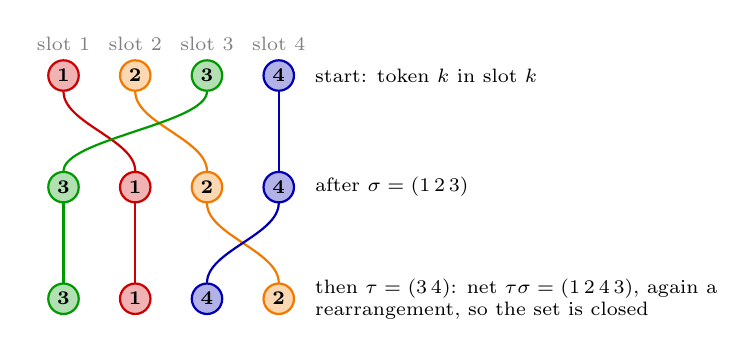
\begin{tikzpicture}[scale=0.675]
  \node[font=\scriptsize,gray] at (1.35,0.6) {slot 1};
  \node[font=\scriptsize,gray] at (2.70,0.6) {slot 2};
  \node[font=\scriptsize,gray] at (4.05,0.6) {slot 3};
  \node[font=\scriptsize,gray] at (5.40,0.6) {slot 4};
  \node[font=\scriptsize\bfseries,circle,inner sep=1pt,minimum size=11pt,fill=red!80!black!30,draw=red!80!black,thick,text=black] at (1.35,0.00) {1};
  \node[font=\scriptsize\bfseries,circle,inner sep=1pt,minimum size=11pt,fill=orange!95!black!30,draw=orange!95!black,thick,text=black] at (2.70,0.00) {2};
  \node[font=\scriptsize\bfseries,circle,inner sep=1pt,minimum size=11pt,fill=green!60!black!30,draw=green!60!black,thick,text=black] at (4.05,0.00) {3};
  \node[font=\scriptsize\bfseries,circle,inner sep=1pt,minimum size=11pt,fill=blue!70!black!30,draw=blue!70!black,thick,text=black] at (5.40,0.00) {4};
  \node[font=\scriptsize,anchor=west,align=left] at (5.90,0.00) {start: token $k$ in slot $k$};
  \draw[thick,red!80!black] (1.35,-0.30) .. controls (1.35,-0.90) and (2.70,-1.20) .. (2.70,-1.80);
  \draw[thick,orange!95!black] (2.70,-0.30) .. controls (2.70,-0.90) and (4.05,-1.20) .. (4.05,-1.80);
  \draw[thick,green!60!black] (4.05,-0.30) .. controls (4.05,-0.90) and (1.35,-1.20) .. (1.35,-1.80);
  \draw[thick,blue!70!black] (5.40,-0.30) .. controls (5.40,-0.90) and (5.40,-1.20) .. (5.40,-1.80);
  \node[font=\scriptsize\bfseries,circle,inner sep=1pt,minimum size=11pt,fill=green!60!black!30,draw=green!60!black,thick,text=black] at (1.35,-2.10) {3};
  \node[font=\scriptsize\bfseries,circle,inner sep=1pt,minimum size=11pt,fill=red!80!black!30,draw=red!80!black,thick,text=black] at (2.70,-2.10) {1};
  \node[font=\scriptsize\bfseries,circle,inner sep=1pt,minimum size=11pt,fill=orange!95!black!30,draw=orange!95!black,thick,text=black] at (4.05,-2.10) {2};
  \node[font=\scriptsize\bfseries,circle,inner sep=1pt,minimum size=11pt,fill=blue!70!black!30,draw=blue!70!black,thick,text=black] at (5.40,-2.10) {4};
  \node[font=\scriptsize,anchor=west,align=left] at (5.90,-2.10) {after $\sigma=(1\,2\,3)$};
  \draw[thick,green!60!black] (1.35,-2.40) .. controls (1.35,-3.00) and (1.35,-3.30) .. (1.35,-3.90);
  \draw[thick,red!80!black] (2.70,-2.40) .. controls (2.70,-3.00) and (2.70,-3.30) .. (2.70,-3.90);
  \draw[thick,orange!95!black] (4.05,-2.40) .. controls (4.05,-3.00) and (5.40,-3.30) .. (5.40,-3.90);
  \draw[thick,blue!70!black] (5.40,-2.40) .. controls (5.40,-3.00) and (4.05,-3.30) .. (4.05,-3.90);
  \node[font=\scriptsize\bfseries,circle,inner sep=1pt,minimum size=11pt,fill=green!60!black!30,draw=green!60!black,thick,text=black] at (1.35,-4.20) {3};
  \node[font=\scriptsize\bfseries,circle,inner sep=1pt,minimum size=11pt,fill=red!80!black!30,draw=red!80!black,thick,text=black] at (2.70,-4.20) {1};
  \node[font=\scriptsize\bfseries,circle,inner sep=1pt,minimum size=11pt,fill=blue!70!black!30,draw=blue!70!black,thick,text=black] at (4.05,-4.20) {4};
  \node[font=\scriptsize\bfseries,circle,inner sep=1pt,minimum size=11pt,fill=orange!95!black!30,draw=orange!95!black,thick,text=black] at (5.40,-4.20) {2};
  \node[font=\scriptsize,anchor=west,align=left] at (5.90,-4.20) {then $\tau=(3\,4)$: net $\tau\sigma=(1\,2\,4\,3)$, again a\\rearrangement, so the set is closed};
\end{tikzpicture}}

\newcommand{\figXu}{%
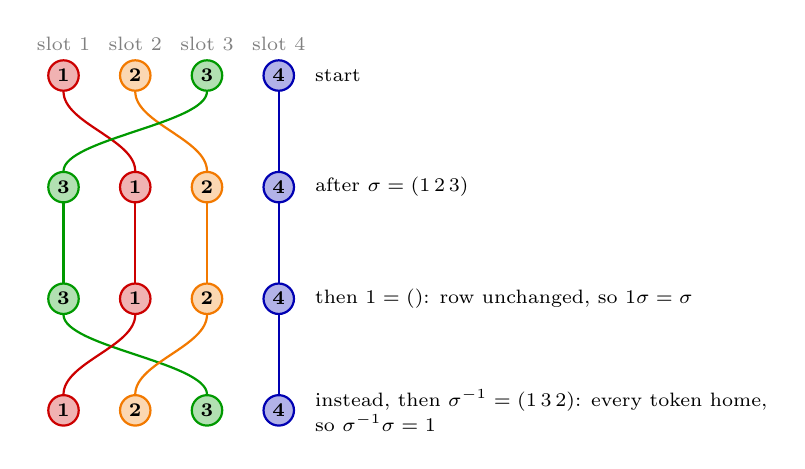
\begin{tikzpicture}[scale=0.675]
  \node[font=\scriptsize,gray] at (1.35,0.6) {slot 1};
  \node[font=\scriptsize,gray] at (2.70,0.6) {slot 2};
  \node[font=\scriptsize,gray] at (4.05,0.6) {slot 3};
  \node[font=\scriptsize,gray] at (5.40,0.6) {slot 4};
  \node[font=\scriptsize\bfseries,circle,inner sep=1pt,minimum size=11pt,fill=red!80!black!30,draw=red!80!black,thick,text=black] at (1.35,0.00) {1};
  \node[font=\scriptsize\bfseries,circle,inner sep=1pt,minimum size=11pt,fill=orange!95!black!30,draw=orange!95!black,thick,text=black] at (2.70,0.00) {2};
  \node[font=\scriptsize\bfseries,circle,inner sep=1pt,minimum size=11pt,fill=green!60!black!30,draw=green!60!black,thick,text=black] at (4.05,0.00) {3};
  \node[font=\scriptsize\bfseries,circle,inner sep=1pt,minimum size=11pt,fill=blue!70!black!30,draw=blue!70!black,thick,text=black] at (5.40,0.00) {4};
  \node[font=\scriptsize,anchor=west,align=left] at (5.90,0.00) {start};
  \draw[thick,red!80!black] (1.35,-0.30) .. controls (1.35,-0.90) and (2.70,-1.20) .. (2.70,-1.80);
  \draw[thick,orange!95!black] (2.70,-0.30) .. controls (2.70,-0.90) and (4.05,-1.20) .. (4.05,-1.80);
  \draw[thick,green!60!black] (4.05,-0.30) .. controls (4.05,-0.90) and (1.35,-1.20) .. (1.35,-1.80);
  \draw[thick,blue!70!black] (5.40,-0.30) .. controls (5.40,-0.90) and (5.40,-1.20) .. (5.40,-1.80);
  \node[font=\scriptsize\bfseries,circle,inner sep=1pt,minimum size=11pt,fill=green!60!black!30,draw=green!60!black,thick,text=black] at (1.35,-2.10) {3};
  \node[font=\scriptsize\bfseries,circle,inner sep=1pt,minimum size=11pt,fill=red!80!black!30,draw=red!80!black,thick,text=black] at (2.70,-2.10) {1};
  \node[font=\scriptsize\bfseries,circle,inner sep=1pt,minimum size=11pt,fill=orange!95!black!30,draw=orange!95!black,thick,text=black] at (4.05,-2.10) {2};
  \node[font=\scriptsize\bfseries,circle,inner sep=1pt,minimum size=11pt,fill=blue!70!black!30,draw=blue!70!black,thick,text=black] at (5.40,-2.10) {4};
  \node[font=\scriptsize,anchor=west,align=left] at (5.90,-2.10) {after $\sigma=(1\,2\,3)$};
  \draw[thick,green!60!black] (1.35,-2.40) .. controls (1.35,-3.00) and (1.35,-3.30) .. (1.35,-3.90);
  \draw[thick,red!80!black] (2.70,-2.40) .. controls (2.70,-3.00) and (2.70,-3.30) .. (2.70,-3.90);
  \draw[thick,orange!95!black] (4.05,-2.40) .. controls (4.05,-3.00) and (4.05,-3.30) .. (4.05,-3.90);
  \draw[thick,blue!70!black] (5.40,-2.40) .. controls (5.40,-3.00) and (5.40,-3.30) .. (5.40,-3.90);
  \node[font=\scriptsize\bfseries,circle,inner sep=1pt,minimum size=11pt,fill=green!60!black!30,draw=green!60!black,thick,text=black] at (1.35,-4.20) {3};
  \node[font=\scriptsize\bfseries,circle,inner sep=1pt,minimum size=11pt,fill=red!80!black!30,draw=red!80!black,thick,text=black] at (2.70,-4.20) {1};
  \node[font=\scriptsize\bfseries,circle,inner sep=1pt,minimum size=11pt,fill=orange!95!black!30,draw=orange!95!black,thick,text=black] at (4.05,-4.20) {2};
  \node[font=\scriptsize\bfseries,circle,inner sep=1pt,minimum size=11pt,fill=blue!70!black!30,draw=blue!70!black,thick,text=black] at (5.40,-4.20) {4};
  \node[font=\scriptsize,anchor=west,align=left] at (5.90,-4.20) {then $1=()$: row unchanged, so $1\sigma=\sigma$};
  \draw[thick,green!60!black] (1.35,-4.50) .. controls (1.35,-5.10) and (4.05,-5.40) .. (4.05,-6.00);
  \draw[thick,red!80!black] (2.70,-4.50) .. controls (2.70,-5.10) and (1.35,-5.40) .. (1.35,-6.00);
  \draw[thick,orange!95!black] (4.05,-4.50) .. controls (4.05,-5.10) and (2.70,-5.40) .. (2.70,-6.00);
  \draw[thick,blue!70!black] (5.40,-4.50) .. controls (5.40,-5.10) and (5.40,-5.40) .. (5.40,-6.00);
  \node[font=\scriptsize\bfseries,circle,inner sep=1pt,minimum size=11pt,fill=red!80!black!30,draw=red!80!black,thick,text=black] at (1.35,-6.30) {1};
  \node[font=\scriptsize\bfseries,circle,inner sep=1pt,minimum size=11pt,fill=orange!95!black!30,draw=orange!95!black,thick,text=black] at (2.70,-6.30) {2};
  \node[font=\scriptsize\bfseries,circle,inner sep=1pt,minimum size=11pt,fill=green!60!black!30,draw=green!60!black,thick,text=black] at (4.05,-6.30) {3};
  \node[font=\scriptsize\bfseries,circle,inner sep=1pt,minimum size=11pt,fill=blue!70!black!30,draw=blue!70!black,thick,text=black] at (5.40,-6.30) {4};
  \node[font=\scriptsize,anchor=west,align=left] at (5.90,-6.30) {instead, then $\sigma^{-1}=(1\,3\,2)$: every token home,\\so $\sigma^{-1}\sigma=1$};
\end{tikzpicture}}

\newcommand{\figXv}{%
\begin{tikzpicture}[scale=0.92]
\begin{scope}[shift={(0.0,0)}]
  \draw[thick,big] (90:1)--(162:1)--(234:1)--(306:1)--(18:1)--cycle;
  \node[font=\scriptsize,fill=white,inner sep=1pt,circle,draw=gray!60] at (90:1) {1};
  \node[font=\scriptsize,fill=white,inner sep=1pt,circle,draw=gray!60] at (162:1) {2};
  \node[font=\scriptsize,fill=white,inner sep=1pt,circle,draw=gray!60] at (234:1) {3};
  \node[font=\scriptsize,fill=white,inner sep=1pt,circle,draw=gray!60] at (306:1) {4};
  \node[font=\scriptsize,fill=white,inner sep=1pt,circle,draw=gray!60] at (378:1) {5};
  \node[font=\scriptsize,align=center] at (0,-1.55) {$1$};
\end{scope}
\begin{scope}[shift={(3.2,0)}]
  \draw[thick,big] (90:1)--(162:1)--(234:1)--(306:1)--(18:1)--cycle;
  \draw[-{Stealth[length=3pt]},mkc,thick] (0.35,0) arc (0:250:0.35);
  \node[font=\scriptsize,fill=white,inner sep=1pt,circle,draw=gray!60] at (162:1) {1};
  \node[font=\scriptsize,fill=white,inner sep=1pt,circle,draw=gray!60] at (234:1) {2};
  \node[font=\scriptsize,fill=white,inner sep=1pt,circle,draw=gray!60] at (306:1) {3};
  \node[font=\scriptsize,fill=white,inner sep=1pt,circle,draw=gray!60] at (378:1) {4};
  \node[font=\scriptsize,fill=white,inner sep=1pt,circle,draw=gray!60] at (90:1) {5};
  \node[font=\scriptsize,align=center] at (0,-1.55) {$st$};
\end{scope}
\begin{scope}[shift={(6.4,0)}]
  \draw[thick,big] (90:1)--(162:1)--(234:1)--(306:1)--(18:1)--cycle;
  \draw[-{Stealth[length=3pt]},mkc,thick] (0.35,0) arc (0:250:0.35);
  \node[font=\scriptsize,fill=white,inner sep=1pt,circle,draw=gray!60] at (234:1) {1};
  \node[font=\scriptsize,fill=white,inner sep=1pt,circle,draw=gray!60] at (306:1) {2};
  \node[font=\scriptsize,fill=white,inner sep=1pt,circle,draw=gray!60] at (378:1) {3};
  \node[font=\scriptsize,fill=white,inner sep=1pt,circle,draw=gray!60] at (90:1) {4};
  \node[font=\scriptsize,fill=white,inner sep=1pt,circle,draw=gray!60] at (162:1) {5};
  \node[font=\scriptsize,align=center] at (0,-1.55) {$(st)^2$};
\end{scope}
\begin{scope}[shift={(9.600000000000001,0)}]
  \draw[thick,big] (90:1)--(162:1)--(234:1)--(306:1)--(18:1)--cycle;
  \draw[-{Stealth[length=3pt]},mkc,thick] (0.35,0) arc (0:250:0.35);
  \node[font=\scriptsize,fill=white,inner sep=1pt,circle,draw=gray!60] at (306:1) {1};
  \node[font=\scriptsize,fill=white,inner sep=1pt,circle,draw=gray!60] at (378:1) {2};
  \node[font=\scriptsize,fill=white,inner sep=1pt,circle,draw=gray!60] at (90:1) {3};
  \node[font=\scriptsize,fill=white,inner sep=1pt,circle,draw=gray!60] at (162:1) {4};
  \node[font=\scriptsize,fill=white,inner sep=1pt,circle,draw=gray!60] at (234:1) {5};
  \node[font=\scriptsize,align=center] at (0,-1.55) {$(st)^3$};
\end{scope}
\begin{scope}[shift={(12.8,0)}]
  \draw[thick,big] (90:1)--(162:1)--(234:1)--(306:1)--(18:1)--cycle;
  \draw[-{Stealth[length=3pt]},mkc,thick] (0.35,0) arc (0:250:0.35);
  \node[font=\scriptsize,fill=white,inner sep=1pt,circle,draw=gray!60] at (378:1) {1};
  \node[font=\scriptsize,fill=white,inner sep=1pt,circle,draw=gray!60] at (90:1) {2};
  \node[font=\scriptsize,fill=white,inner sep=1pt,circle,draw=gray!60] at (162:1) {3};
  \node[font=\scriptsize,fill=white,inner sep=1pt,circle,draw=gray!60] at (234:1) {4};
  \node[font=\scriptsize,fill=white,inner sep=1pt,circle,draw=gray!60] at (306:1) {5};
  \node[font=\scriptsize,align=center] at (0,-1.55) {$(st)^4$};
\end{scope}
\begin{scope}[shift={(0.0,-3.6)}]
  \draw[thick,big] (90:1)--(162:1)--(234:1)--(306:1)--(18:1)--cycle;
  \draw[dashed,pit] (126:1.35)--(306:1.35);
  \node[font=\scriptsize,fill=white,inner sep=1pt,circle,draw=gray!60] at (162:1) {1};
  \node[font=\scriptsize,fill=white,inner sep=1pt,circle,draw=gray!60] at (90:1) {2};
  \node[font=\scriptsize,fill=white,inner sep=1pt,circle,draw=gray!60] at (378:1) {3};
  \node[font=\scriptsize,fill=white,inner sep=1pt,circle,draw=gray!60] at (306:1) {4};
  \node[font=\scriptsize,fill=white,inner sep=1pt,circle,draw=gray!60] at (234:1) {5};
  \node[font=\scriptsize,align=center] at (0,-1.55) {$s$};
\end{scope}
\begin{scope}[shift={(3.2,-3.6)}]
  \draw[thick,big] (90:1)--(162:1)--(234:1)--(306:1)--(18:1)--cycle;
  \draw[dashed,pit] (90:1.35)--(270:1.35);
  \node[font=\scriptsize,fill=white,inner sep=1pt,circle,draw=gray!60] at (90:1) {1};
  \node[font=\scriptsize,fill=white,inner sep=1pt,circle,draw=gray!60] at (378:1) {2};
  \node[font=\scriptsize,fill=white,inner sep=1pt,circle,draw=gray!60] at (306:1) {3};
  \node[font=\scriptsize,fill=white,inner sep=1pt,circle,draw=gray!60] at (234:1) {4};
  \node[font=\scriptsize,fill=white,inner sep=1pt,circle,draw=gray!60] at (162:1) {5};
  \node[font=\scriptsize,align=center] at (0,-1.55) {$t$};
\end{scope}
\begin{scope}[shift={(6.4,-3.6)}]
  \draw[thick,big] (90:1)--(162:1)--(234:1)--(306:1)--(18:1)--cycle;
  \draw[dashed,pit] (54:1.35)--(234:1.35);
  \node[font=\scriptsize,fill=white,inner sep=1pt,circle,draw=gray!60] at (378:1) {1};
  \node[font=\scriptsize,fill=white,inner sep=1pt,circle,draw=gray!60] at (306:1) {2};
  \node[font=\scriptsize,fill=white,inner sep=1pt,circle,draw=gray!60] at (234:1) {3};
  \node[font=\scriptsize,fill=white,inner sep=1pt,circle,draw=gray!60] at (162:1) {4};
  \node[font=\scriptsize,fill=white,inner sep=1pt,circle,draw=gray!60] at (90:1) {5};
  \node[font=\scriptsize,align=center] at (0,-1.55) {$tst$};
\end{scope}
\begin{scope}[shift={(9.600000000000001,-3.6)}]
  \draw[thick,big] (90:1)--(162:1)--(234:1)--(306:1)--(18:1)--cycle;
  \draw[dashed,pit] (18:1.35)--(198:1.35);
  \node[font=\scriptsize,fill=white,inner sep=1pt,circle,draw=gray!60] at (306:1) {1};
  \node[font=\scriptsize,fill=white,inner sep=1pt,circle,draw=gray!60] at (234:1) {2};
  \node[font=\scriptsize,fill=white,inner sep=1pt,circle,draw=gray!60] at (162:1) {3};
  \node[font=\scriptsize,fill=white,inner sep=1pt,circle,draw=gray!60] at (90:1) {4};
  \node[font=\scriptsize,fill=white,inner sep=1pt,circle,draw=gray!60] at (378:1) {5};
  \node[font=\scriptsize,align=center] at (0,-1.55) {$tstst$};
\end{scope}
\begin{scope}[shift={(12.8,-3.6)}]
  \draw[thick,big] (90:1)--(162:1)--(234:1)--(306:1)--(18:1)--cycle;
  \draw[dashed,pit] (-18:1.35)--(162:1.35);
  \node[font=\scriptsize,fill=white,inner sep=1pt,circle,draw=gray!60] at (234:1) {1};
  \node[font=\scriptsize,fill=white,inner sep=1pt,circle,draw=gray!60] at (162:1) {2};
  \node[font=\scriptsize,fill=white,inner sep=1pt,circle,draw=gray!60] at (90:1) {3};
  \node[font=\scriptsize,fill=white,inner sep=1pt,circle,draw=gray!60] at (378:1) {4};
  \node[font=\scriptsize,fill=white,inner sep=1pt,circle,draw=gray!60] at (306:1) {5};
  \node[font=\scriptsize,align=center] at (0,-1.55) {$tststst$};
\end{scope}
\end{tikzpicture}}

\newcommand{\figXw}{%
\begin{tikzpicture}[scale=0.812,>={Stealth[length=4pt]}]
  \foreach \k in {1,...,6} {\fill (\k*1.3,0) circle (2pt); \node[font=\scriptsize,below=2pt] at (\k*1.3,0) {\k};}
  \draw[->,thick,red!80!black] (1.3,0.1) to[bend left=50] (2.6,0.1);
  \draw[->,thick,red!80!black] (2.6,0.1) to[bend left=50] (5.2,0.1);
  \draw[->,thick,red!80!black] (5.2,-0.1) to[bend left=35] (1.3,-0.1);
  \draw[->,thick,blue!70!black] (3.9,0.1) to[bend left=50] (6.5,0.1);
  \draw[->,thick,blue!70!black] (6.5,-0.1) to[bend left=50] (3.9,-0.1);
  \draw[->,thick,gray] (7.8,0.1) to[out=60,in=120,looseness=6] (7.8,0.1);
  \node[font=\scriptsize,red!80!black] at (3.3,1.0) {$(1\,2\,4)$}; \node[font=\scriptsize,blue!70!black] at (5.2,-1.0) {$(3\,5)$}; \node[font=\scriptsize,gray] at (7.8,1.0) {6 fixed};
\end{tikzpicture}}

\newcommand{\figXx}{%
\begin{tikzpicture}[scale=0.562,>={Stealth[length=4pt]}]
  \foreach \dx/\st/\nm in {0/1/(1\,2\,4), 5.2/2/(2\,4\,1), 10.4/4/(4\,1\,2)} {
    \begin{scope}[shift={(\dx,0)}]
      \coordinate (p1) at (90:1.2); \coordinate (p2) at (210:1.2); \coordinate (p4) at (330:1.2);
      \draw[->,thick,red!80!black] (p1) to[bend right=25] (p2);
      \draw[->,thick,red!80!black] (p2) to[bend right=25] (p4);
      \draw[->,thick,red!80!black] (p4) to[bend right=25] (p1);
      \node[font=\scriptsize,circle,fill=white,draw=gray,inner sep=1pt] at (p1) {1};
      \node[font=\scriptsize,circle,fill=white,draw=gray,inner sep=1pt] at (p2) {2};
      \node[font=\scriptsize,circle,fill=white,draw=gray,inner sep=1pt] at (p4) {4};
      \node[font=\scriptsize,mkc] at (0,-2.0) {start at \st: $\nm$};
    \end{scope}
  }
  \draw[very thick,mkc] (90:1.2) circle (0.32);
  \draw[very thick,mkc] ($(5.2,0)+(210:1.2)$) circle (0.32);
  \draw[very thick,mkc] ($(10.4,0)+(330:1.2)$) circle (0.32);
\end{tikzpicture}}

\newcommand{\figXy}{%
\begin{tikzpicture}[>={Stealth[length=4pt]},x=1cm,y=0.42cm]
  \node[font=\scriptsize,gray] at (0,1.1) {start}; \node[font=\scriptsize,gray] at (2.6,1.1) {after $(1\,2\,4)(3\,5)$}; \node[font=\scriptsize,gray] at (5.2,1.1) {after $(2\,6)$};
  \node[font=\small\bfseries,circle,inner sep=1pt,minimum size=12pt,fill=red!80!black!30,draw=red!80!black,thick] at (0,-1) {1};
  \node[font=\small\bfseries,circle,inner sep=1pt,minimum size=12pt,fill=red!80!black!30,draw=red!80!black,thick] at (2.6,-1) {2};
  \node[font=\small\bfseries,circle,inner sep=1pt,minimum size=12pt,fill=red!80!black!30,draw=red!80!black,thick] at (5.2,-1) {6};
  \draw[->,thick,red!80!black] (0.4,-1) -- (2.2,-1);
  \draw[->,thick,red!80!black] (3.0,-1) -- (4.8,-1);
  \node[font=\scriptsize,gray,anchor=west] at (5.7,-1) {so $1\to6$};
  \node[font=\small\bfseries,circle,inner sep=1pt,minimum size=12pt,fill=orange!95!black!30,draw=orange!95!black,thick] at (0,-2) {2};
  \node[font=\small\bfseries,circle,inner sep=1pt,minimum size=12pt,fill=orange!95!black!30,draw=orange!95!black,thick] at (2.6,-2) {4};
  \node[font=\small\bfseries,circle,inner sep=1pt,minimum size=12pt,fill=orange!95!black!30,draw=orange!95!black,thick] at (5.2,-2) {4};
  \draw[->,thick,orange!95!black] (0.4,-2) -- (2.2,-2);
  \draw[->,thick,orange!95!black] (3.0,-2) -- (4.8,-2);
  \node[font=\scriptsize,gray,anchor=west] at (5.7,-2) {so $2\to4$};
  \node[font=\small\bfseries,circle,inner sep=1pt,minimum size=12pt,fill=green!60!black!30,draw=green!60!black,thick] at (0,-3) {3};
  \node[font=\small\bfseries,circle,inner sep=1pt,minimum size=12pt,fill=green!60!black!30,draw=green!60!black,thick] at (2.6,-3) {5};
  \node[font=\small\bfseries,circle,inner sep=1pt,minimum size=12pt,fill=green!60!black!30,draw=green!60!black,thick] at (5.2,-3) {5};
  \draw[->,thick,green!60!black] (0.4,-3) -- (2.2,-3);
  \draw[->,thick,green!60!black] (3.0,-3) -- (4.8,-3);
  \node[font=\scriptsize,gray,anchor=west] at (5.7,-3) {so $3\to5$};
  \node[font=\small\bfseries,circle,inner sep=1pt,minimum size=12pt,fill=blue!70!black!30,draw=blue!70!black,thick] at (0,-4) {4};
  \node[font=\small\bfseries,circle,inner sep=1pt,minimum size=12pt,fill=blue!70!black!30,draw=blue!70!black,thick] at (2.6,-4) {1};
  \node[font=\small\bfseries,circle,inner sep=1pt,minimum size=12pt,fill=blue!70!black!30,draw=blue!70!black,thick] at (5.2,-4) {1};
  \draw[->,thick,blue!70!black] (0.4,-4) -- (2.2,-4);
  \draw[->,thick,blue!70!black] (3.0,-4) -- (4.8,-4);
  \node[font=\scriptsize,gray,anchor=west] at (5.7,-4) {so $4\to1$};
  \node[font=\small\bfseries,circle,inner sep=1pt,minimum size=12pt,fill=violet!30,draw=violet,thick] at (0,-5) {5};
  \node[font=\small\bfseries,circle,inner sep=1pt,minimum size=12pt,fill=violet!30,draw=violet,thick] at (2.6,-5) {3};
  \node[font=\small\bfseries,circle,inner sep=1pt,minimum size=12pt,fill=violet!30,draw=violet,thick] at (5.2,-5) {3};
  \draw[->,thick,violet] (0.4,-5) -- (2.2,-5);
  \draw[->,thick,violet] (3.0,-5) -- (4.8,-5);
  \node[font=\scriptsize,gray,anchor=west] at (5.7,-5) {so $5\to3$};
  \node[font=\small\bfseries,circle,inner sep=1pt,minimum size=12pt,fill=gray!70!black!30,draw=gray!70!black,thick] at (0,-6) {6};
  \node[font=\small\bfseries,circle,inner sep=1pt,minimum size=12pt,fill=gray!70!black!30,draw=gray!70!black,thick] at (2.6,-6) {6};
  \node[font=\small\bfseries,circle,inner sep=1pt,minimum size=12pt,fill=gray!70!black!30,draw=gray!70!black,thick] at (5.2,-6) {2};
  \draw[->,thick,gray!70!black] (0.4,-6) -- (2.2,-6);
  \draw[->,thick,gray!70!black] (3.0,-6) -- (4.8,-6);
  \node[font=\scriptsize,gray,anchor=west] at (5.7,-6) {so $6\to2$};
  \node[font=\scriptsize,mkc] at (1.3,-0.3) {first factor}; \node[font=\scriptsize,mkc] at (3.9,-0.3) {second factor};
\end{tikzpicture}}

\newcommand{\figXz}{%
\begin{tikzpicture}[scale=1.000,>={Stealth[length=4pt]}]
  \fill (1.3,0) circle (2pt); \node[font=\scriptsize,below=3pt] at (1.3,0) {1};
  \fill (2.6,0) circle (2pt); \node[font=\scriptsize,below=3pt] at (2.6,0) {2};
  \fill (3.9000000000000004,0) circle (2pt); \node[font=\scriptsize,below=3pt] at (3.9000000000000004,0) {3};
  \fill (5.2,0) circle (2pt); \node[font=\scriptsize,below=3pt] at (5.2,0) {4};
  \fill (6.5,0) circle (2pt); \node[font=\scriptsize,below=3pt] at (6.5,0) {5};
  \fill (7.800000000000001,0) circle (2pt); \node[font=\scriptsize,below=3pt] at (7.800000000000001,0) {6};
  \draw[->,thick,red!80!black] (1.3,0.1) to[bend left=45] (7.800000000000001,0.1);
  \draw[->,thick,red!80!black] (7.800000000000001,-0.1) to[bend left=45] (2.6,-0.1);
  \draw[->,thick,red!80!black] (2.6,0.1) to[bend left=45] (5.2,0.1);
  \draw[->,thick,red!80!black] (5.2,-0.1) to[bend left=45] (1.3,-0.1);
  \node[font=\scriptsize,red!80!black] at (4.55,1.55) {$(1\,6\,2\,4)$};
  \draw[->,thick,blue!70!black] (3.9000000000000004,0.1) to[bend left=45] (6.5,0.1);
  \draw[->,thick,blue!70!black] (6.5,-0.1) to[bend left=45] (3.9000000000000004,-0.1);
  \node[font=\scriptsize,blue!70!black] at (5.2,-1.05) {$(3\,5)$};
\end{tikzpicture}}

\newcommand{\figXaa}{%
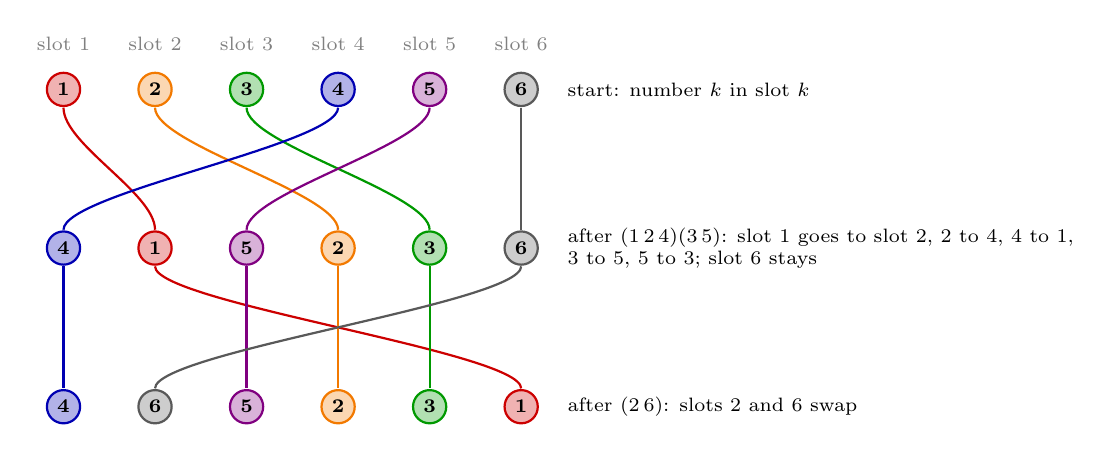
\begin{tikzpicture}[scale=0.775]
  \node[font=\scriptsize,gray] at (1.5,0.75) {slot 1};
  \node[font=\scriptsize,gray] at (3.0,0.75) {slot 2};
  \node[font=\scriptsize,gray] at (4.5,0.75) {slot 3};
  \node[font=\scriptsize,gray] at (6.0,0.75) {slot 4};
  \node[font=\scriptsize,gray] at (7.5,0.75) {slot 5};
  \node[font=\scriptsize,gray] at (9.0,0.75) {slot 6};
  \node[font=\scriptsize\bfseries,circle,inner sep=1pt,minimum size=12pt,fill=red!80!black!30,draw=red!80!black,thick,text=black] at (1.5,0.0) {1};
  \node[font=\scriptsize\bfseries,circle,inner sep=1pt,minimum size=12pt,fill=orange!95!black!30,draw=orange!95!black,thick,text=black] at (3.0,0.0) {2};
  \node[font=\scriptsize\bfseries,circle,inner sep=1pt,minimum size=12pt,fill=green!60!black!30,draw=green!60!black,thick,text=black] at (4.5,0.0) {3};
  \node[font=\scriptsize\bfseries,circle,inner sep=1pt,minimum size=12pt,fill=blue!70!black!30,draw=blue!70!black,thick,text=black] at (6.0,0.0) {4};
  \node[font=\scriptsize\bfseries,circle,inner sep=1pt,minimum size=12pt,fill=violet!30,draw=violet,thick,text=black] at (7.5,0.0) {5};
  \node[font=\scriptsize\bfseries,circle,inner sep=1pt,minimum size=12pt,fill=gray!70!black!30,draw=gray!70!black,thick,text=black] at (9.0,0.0) {6};
  \node[font=\scriptsize,anchor=west,align=left] at (9.6,0.0) {start: number $k$ in slot $k$};
  \draw[thick,red!80!black] (1.5,-0.3) .. controls (1.5,-0.9) and (3.0,-1.7000000000000002) .. (3.0,-2.3000000000000003);
  \draw[thick,orange!95!black] (3.0,-0.3) .. controls (3.0,-0.9) and (6.0,-1.7000000000000002) .. (6.0,-2.3000000000000003);
  \draw[thick,green!60!black] (4.5,-0.3) .. controls (4.5,-0.9) and (7.5,-1.7000000000000002) .. (7.5,-2.3000000000000003);
  \draw[thick,blue!70!black] (6.0,-0.3) .. controls (6.0,-0.9) and (1.5,-1.7000000000000002) .. (1.5,-2.3000000000000003);
  \draw[thick,violet] (7.5,-0.3) .. controls (7.5,-0.9) and (4.5,-1.7000000000000002) .. (4.5,-2.3000000000000003);
  \draw[thick,gray!70!black] (9.0,-0.3) .. controls (9.0,-0.9) and (9.0,-1.7000000000000002) .. (9.0,-2.3000000000000003);
  \node[font=\scriptsize\bfseries,circle,inner sep=1pt,minimum size=12pt,fill=blue!70!black!30,draw=blue!70!black,thick,text=black] at (1.5,-2.6) {4};
  \node[font=\scriptsize\bfseries,circle,inner sep=1pt,minimum size=12pt,fill=red!80!black!30,draw=red!80!black,thick,text=black] at (3.0,-2.6) {1};
  \node[font=\scriptsize\bfseries,circle,inner sep=1pt,minimum size=12pt,fill=violet!30,draw=violet,thick,text=black] at (4.5,-2.6) {5};
  \node[font=\scriptsize\bfseries,circle,inner sep=1pt,minimum size=12pt,fill=orange!95!black!30,draw=orange!95!black,thick,text=black] at (6.0,-2.6) {2};
  \node[font=\scriptsize\bfseries,circle,inner sep=1pt,minimum size=12pt,fill=green!60!black!30,draw=green!60!black,thick,text=black] at (7.5,-2.6) {3};
  \node[font=\scriptsize\bfseries,circle,inner sep=1pt,minimum size=12pt,fill=gray!70!black!30,draw=gray!70!black,thick,text=black] at (9.0,-2.6) {6};
  \node[font=\scriptsize,anchor=west,align=left] at (9.6,-2.6) {after $(1\,2\,4)(3\,5)$: slot 1 goes to slot 2, 2 to 4, 4 to 1,\\3 to 5, 5 to 3; slot 6 stays};
  \draw[thick,blue!70!black] (1.5,-2.9) .. controls (1.5,-3.5) and (1.5,-4.3) .. (1.5,-4.9);
  \draw[thick,red!80!black] (3.0,-2.9) .. controls (3.0,-3.5) and (9.0,-4.3) .. (9.0,-4.9);
  \draw[thick,violet] (4.5,-2.9) .. controls (4.5,-3.5) and (4.5,-4.3) .. (4.5,-4.9);
  \draw[thick,orange!95!black] (6.0,-2.9) .. controls (6.0,-3.5) and (6.0,-4.3) .. (6.0,-4.9);
  \draw[thick,green!60!black] (7.5,-2.9) .. controls (7.5,-3.5) and (7.5,-4.3) .. (7.5,-4.9);
  \draw[thick,gray!70!black] (9.0,-2.9) .. controls (9.0,-3.5) and (3.0,-4.3) .. (3.0,-4.9);
  \node[font=\scriptsize\bfseries,circle,inner sep=1pt,minimum size=12pt,fill=blue!70!black!30,draw=blue!70!black,thick,text=black] at (1.5,-5.2) {4};
  \node[font=\scriptsize\bfseries,circle,inner sep=1pt,minimum size=12pt,fill=gray!70!black!30,draw=gray!70!black,thick,text=black] at (3.0,-5.2) {6};
  \node[font=\scriptsize\bfseries,circle,inner sep=1pt,minimum size=12pt,fill=violet!30,draw=violet,thick,text=black] at (4.5,-5.2) {5};
  \node[font=\scriptsize\bfseries,circle,inner sep=1pt,minimum size=12pt,fill=orange!95!black!30,draw=orange!95!black,thick,text=black] at (6.0,-5.2) {2};
  \node[font=\scriptsize\bfseries,circle,inner sep=1pt,minimum size=12pt,fill=green!60!black!30,draw=green!60!black,thick,text=black] at (7.5,-5.2) {3};
  \node[font=\scriptsize\bfseries,circle,inner sep=1pt,minimum size=12pt,fill=red!80!black!30,draw=red!80!black,thick,text=black] at (9.0,-5.2) {1};
  \node[font=\scriptsize,anchor=west,align=left] at (9.6,-5.2) {after $(2\,6)$: slots 2 and 6 swap};
\end{tikzpicture}}

\newcommand{\figXab}{%
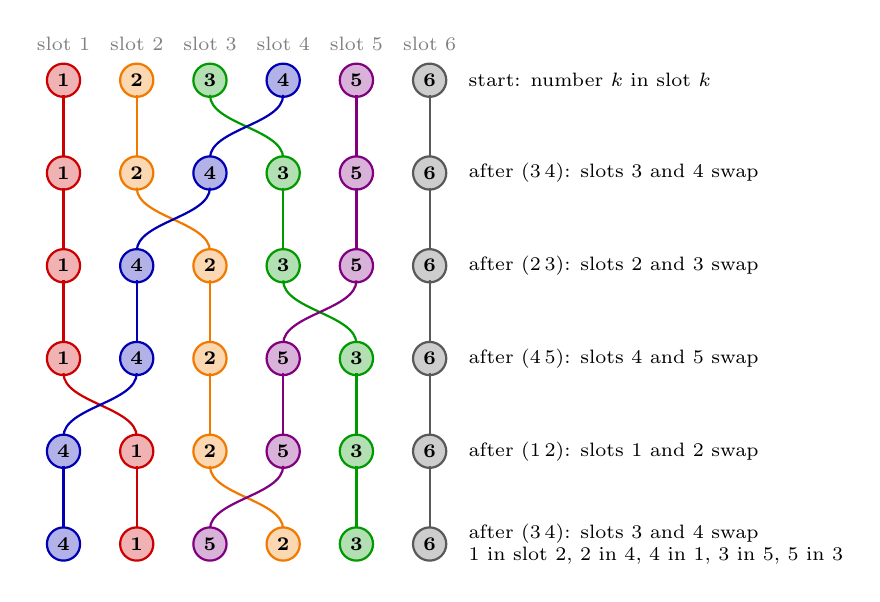
\begin{tikzpicture}[scale=0.62]
  \node[font=\scriptsize,gray] at (1.5,0.75) {slot 1};
  \node[font=\scriptsize,gray] at (3.0,0.75) {slot 2};
  \node[font=\scriptsize,gray] at (4.5,0.75) {slot 3};
  \node[font=\scriptsize,gray] at (6.0,0.75) {slot 4};
  \node[font=\scriptsize,gray] at (7.5,0.75) {slot 5};
  \node[font=\scriptsize,gray] at (9.0,0.75) {slot 6};
  \node[font=\scriptsize\bfseries,circle,inner sep=1pt,minimum size=12pt,fill=red!80!black!30,draw=red!80!black,thick,text=black] at (1.5,0.0) {1};
  \node[font=\scriptsize\bfseries,circle,inner sep=1pt,minimum size=12pt,fill=orange!95!black!30,draw=orange!95!black,thick,text=black] at (3.0,0.0) {2};
  \node[font=\scriptsize\bfseries,circle,inner sep=1pt,minimum size=12pt,fill=green!60!black!30,draw=green!60!black,thick,text=black] at (4.5,0.0) {3};
  \node[font=\scriptsize\bfseries,circle,inner sep=1pt,minimum size=12pt,fill=blue!70!black!30,draw=blue!70!black,thick,text=black] at (6.0,0.0) {4};
  \node[font=\scriptsize\bfseries,circle,inner sep=1pt,minimum size=12pt,fill=violet!30,draw=violet,thick,text=black] at (7.5,0.0) {5};
  \node[font=\scriptsize\bfseries,circle,inner sep=1pt,minimum size=12pt,fill=gray!70!black!30,draw=gray!70!black,thick,text=black] at (9.0,0.0) {6};
  \node[font=\scriptsize,anchor=west,align=left] at (9.6,0.0) {start: number $k$ in slot $k$};
  \draw[thick,red!80!black] (1.5,-0.3) .. controls (1.5,-0.9) and (1.5,-0.9999999999999999) .. (1.5,-1.5999999999999999);
  \draw[thick,orange!95!black] (3.0,-0.3) .. controls (3.0,-0.9) and (3.0,-0.9999999999999999) .. (3.0,-1.5999999999999999);
  \draw[thick,green!60!black] (4.5,-0.3) .. controls (4.5,-0.9) and (6.0,-0.9999999999999999) .. (6.0,-1.5999999999999999);
  \draw[thick,blue!70!black] (6.0,-0.3) .. controls (6.0,-0.9) and (4.5,-0.9999999999999999) .. (4.5,-1.5999999999999999);
  \draw[thick,violet] (7.5,-0.3) .. controls (7.5,-0.9) and (7.5,-0.9999999999999999) .. (7.5,-1.5999999999999999);
  \draw[thick,gray!70!black] (9.0,-0.3) .. controls (9.0,-0.9) and (9.0,-0.9999999999999999) .. (9.0,-1.5999999999999999);
  \node[font=\scriptsize\bfseries,circle,inner sep=1pt,minimum size=12pt,fill=red!80!black!30,draw=red!80!black,thick,text=black] at (1.5,-1.9) {1};
  \node[font=\scriptsize\bfseries,circle,inner sep=1pt,minimum size=12pt,fill=orange!95!black!30,draw=orange!95!black,thick,text=black] at (3.0,-1.9) {2};
  \node[font=\scriptsize\bfseries,circle,inner sep=1pt,minimum size=12pt,fill=blue!70!black!30,draw=blue!70!black,thick,text=black] at (4.5,-1.9) {4};
  \node[font=\scriptsize\bfseries,circle,inner sep=1pt,minimum size=12pt,fill=green!60!black!30,draw=green!60!black,thick,text=black] at (6.0,-1.9) {3};
  \node[font=\scriptsize\bfseries,circle,inner sep=1pt,minimum size=12pt,fill=violet!30,draw=violet,thick,text=black] at (7.5,-1.9) {5};
  \node[font=\scriptsize\bfseries,circle,inner sep=1pt,minimum size=12pt,fill=gray!70!black!30,draw=gray!70!black,thick,text=black] at (9.0,-1.9) {6};
  \node[font=\scriptsize,anchor=west,align=left] at (9.6,-1.9) {after $(3\,4)$: slots 3 and 4 swap};
  \draw[thick,red!80!black] (1.5,-2.1999999999999997) .. controls (1.5,-2.8) and (1.5,-2.9) .. (1.5,-3.5);
  \draw[thick,orange!95!black] (3.0,-2.1999999999999997) .. controls (3.0,-2.8) and (4.5,-2.9) .. (4.5,-3.5);
  \draw[thick,blue!70!black] (4.5,-2.1999999999999997) .. controls (4.5,-2.8) and (3.0,-2.9) .. (3.0,-3.5);
  \draw[thick,green!60!black] (6.0,-2.1999999999999997) .. controls (6.0,-2.8) and (6.0,-2.9) .. (6.0,-3.5);
  \draw[thick,violet] (7.5,-2.1999999999999997) .. controls (7.5,-2.8) and (7.5,-2.9) .. (7.5,-3.5);
  \draw[thick,gray!70!black] (9.0,-2.1999999999999997) .. controls (9.0,-2.8) and (9.0,-2.9) .. (9.0,-3.5);
  \node[font=\scriptsize\bfseries,circle,inner sep=1pt,minimum size=12pt,fill=red!80!black!30,draw=red!80!black,thick,text=black] at (1.5,-3.8) {1};
  \node[font=\scriptsize\bfseries,circle,inner sep=1pt,minimum size=12pt,fill=blue!70!black!30,draw=blue!70!black,thick,text=black] at (3.0,-3.8) {4};
  \node[font=\scriptsize\bfseries,circle,inner sep=1pt,minimum size=12pt,fill=orange!95!black!30,draw=orange!95!black,thick,text=black] at (4.5,-3.8) {2};
  \node[font=\scriptsize\bfseries,circle,inner sep=1pt,minimum size=12pt,fill=green!60!black!30,draw=green!60!black,thick,text=black] at (6.0,-3.8) {3};
  \node[font=\scriptsize\bfseries,circle,inner sep=1pt,minimum size=12pt,fill=violet!30,draw=violet,thick,text=black] at (7.5,-3.8) {5};
  \node[font=\scriptsize\bfseries,circle,inner sep=1pt,minimum size=12pt,fill=gray!70!black!30,draw=gray!70!black,thick,text=black] at (9.0,-3.8) {6};
  \node[font=\scriptsize,anchor=west,align=left] at (9.6,-3.8) {after $(2\,3)$: slots 2 and 3 swap};
  \draw[thick,red!80!black] (1.5,-4.1) .. controls (1.5,-4.7) and (1.5,-4.799999999999999) .. (1.5,-5.3999999999999995);
  \draw[thick,blue!70!black] (3.0,-4.1) .. controls (3.0,-4.7) and (3.0,-4.799999999999999) .. (3.0,-5.3999999999999995);
  \draw[thick,orange!95!black] (4.5,-4.1) .. controls (4.5,-4.7) and (4.5,-4.799999999999999) .. (4.5,-5.3999999999999995);
  \draw[thick,green!60!black] (6.0,-4.1) .. controls (6.0,-4.7) and (7.5,-4.799999999999999) .. (7.5,-5.3999999999999995);
  \draw[thick,violet] (7.5,-4.1) .. controls (7.5,-4.7) and (6.0,-4.799999999999999) .. (6.0,-5.3999999999999995);
  \draw[thick,gray!70!black] (9.0,-4.1) .. controls (9.0,-4.7) and (9.0,-4.799999999999999) .. (9.0,-5.3999999999999995);
  \node[font=\scriptsize\bfseries,circle,inner sep=1pt,minimum size=12pt,fill=red!80!black!30,draw=red!80!black,thick,text=black] at (1.5,-5.699999999999999) {1};
  \node[font=\scriptsize\bfseries,circle,inner sep=1pt,minimum size=12pt,fill=blue!70!black!30,draw=blue!70!black,thick,text=black] at (3.0,-5.699999999999999) {4};
  \node[font=\scriptsize\bfseries,circle,inner sep=1pt,minimum size=12pt,fill=orange!95!black!30,draw=orange!95!black,thick,text=black] at (4.5,-5.699999999999999) {2};
  \node[font=\scriptsize\bfseries,circle,inner sep=1pt,minimum size=12pt,fill=violet!30,draw=violet,thick,text=black] at (6.0,-5.699999999999999) {5};
  \node[font=\scriptsize\bfseries,circle,inner sep=1pt,minimum size=12pt,fill=green!60!black!30,draw=green!60!black,thick,text=black] at (7.5,-5.699999999999999) {3};
  \node[font=\scriptsize\bfseries,circle,inner sep=1pt,minimum size=12pt,fill=gray!70!black!30,draw=gray!70!black,thick,text=black] at (9.0,-5.699999999999999) {6};
  \node[font=\scriptsize,anchor=west,align=left] at (9.6,-5.699999999999999) {after $(4\,5)$: slots 4 and 5 swap};
  \draw[thick,red!80!black] (1.5,-5.999999999999999) .. controls (1.5,-6.6) and (3.0,-6.699999999999999) .. (3.0,-7.3);
  \draw[thick,blue!70!black] (3.0,-5.999999999999999) .. controls (3.0,-6.6) and (1.5,-6.699999999999999) .. (1.5,-7.3);
  \draw[thick,orange!95!black] (4.5,-5.999999999999999) .. controls (4.5,-6.6) and (4.5,-6.699999999999999) .. (4.5,-7.3);
  \draw[thick,violet] (6.0,-5.999999999999999) .. controls (6.0,-6.6) and (6.0,-6.699999999999999) .. (6.0,-7.3);
  \draw[thick,green!60!black] (7.5,-5.999999999999999) .. controls (7.5,-6.6) and (7.5,-6.699999999999999) .. (7.5,-7.3);
  \draw[thick,gray!70!black] (9.0,-5.999999999999999) .. controls (9.0,-6.6) and (9.0,-6.699999999999999) .. (9.0,-7.3);
  \node[font=\scriptsize\bfseries,circle,inner sep=1pt,minimum size=12pt,fill=blue!70!black!30,draw=blue!70!black,thick,text=black] at (1.5,-7.6) {4};
  \node[font=\scriptsize\bfseries,circle,inner sep=1pt,minimum size=12pt,fill=red!80!black!30,draw=red!80!black,thick,text=black] at (3.0,-7.6) {1};
  \node[font=\scriptsize\bfseries,circle,inner sep=1pt,minimum size=12pt,fill=orange!95!black!30,draw=orange!95!black,thick,text=black] at (4.5,-7.6) {2};
  \node[font=\scriptsize\bfseries,circle,inner sep=1pt,minimum size=12pt,fill=violet!30,draw=violet,thick,text=black] at (6.0,-7.6) {5};
  \node[font=\scriptsize\bfseries,circle,inner sep=1pt,minimum size=12pt,fill=green!60!black!30,draw=green!60!black,thick,text=black] at (7.5,-7.6) {3};
  \node[font=\scriptsize\bfseries,circle,inner sep=1pt,minimum size=12pt,fill=gray!70!black!30,draw=gray!70!black,thick,text=black] at (9.0,-7.6) {6};
  \node[font=\scriptsize,anchor=west,align=left] at (9.6,-7.6) {after $(1\,2)$: slots 1 and 2 swap};
  \draw[thick,blue!70!black] (1.5,-7.8999999999999995) .. controls (1.5,-8.5) and (1.5,-8.6) .. (1.5,-9.2);
  \draw[thick,red!80!black] (3.0,-7.8999999999999995) .. controls (3.0,-8.5) and (3.0,-8.6) .. (3.0,-9.2);
  \draw[thick,orange!95!black] (4.5,-7.8999999999999995) .. controls (4.5,-8.5) and (6.0,-8.6) .. (6.0,-9.2);
  \draw[thick,violet] (6.0,-7.8999999999999995) .. controls (6.0,-8.5) and (4.5,-8.6) .. (4.5,-9.2);
  \draw[thick,green!60!black] (7.5,-7.8999999999999995) .. controls (7.5,-8.5) and (7.5,-8.6) .. (7.5,-9.2);
  \draw[thick,gray!70!black] (9.0,-7.8999999999999995) .. controls (9.0,-8.5) and (9.0,-8.6) .. (9.0,-9.2);
  \node[font=\scriptsize\bfseries,circle,inner sep=1pt,minimum size=12pt,fill=blue!70!black!30,draw=blue!70!black,thick,text=black] at (1.5,-9.5) {4};
  \node[font=\scriptsize\bfseries,circle,inner sep=1pt,minimum size=12pt,fill=red!80!black!30,draw=red!80!black,thick,text=black] at (3.0,-9.5) {1};
  \node[font=\scriptsize\bfseries,circle,inner sep=1pt,minimum size=12pt,fill=violet!30,draw=violet,thick,text=black] at (4.5,-9.5) {5};
  \node[font=\scriptsize\bfseries,circle,inner sep=1pt,minimum size=12pt,fill=orange!95!black!30,draw=orange!95!black,thick,text=black] at (6.0,-9.5) {2};
  \node[font=\scriptsize\bfseries,circle,inner sep=1pt,minimum size=12pt,fill=green!60!black!30,draw=green!60!black,thick,text=black] at (7.5,-9.5) {3};
  \node[font=\scriptsize\bfseries,circle,inner sep=1pt,minimum size=12pt,fill=gray!70!black!30,draw=gray!70!black,thick,text=black] at (9.0,-9.5) {6};
  \node[font=\scriptsize,anchor=west,align=left] at (9.6,-9.5) {after $(3\,4)$: slots 3 and 4 swap\\$1$ in slot 2, $2$ in 4, $4$ in 1, $3$ in 5, $5$ in 3};
\end{tikzpicture}}

\newcommand{\figXac}{%
\begin{tikzpicture}[scale=0.8,>={Stealth[length=4pt]}]
  \fill (1.3,0) circle (2pt); \node[font=\scriptsize,below=3pt] at (1.3,0) {1};
  \fill (2.6,0) circle (2pt); \node[font=\scriptsize,below=3pt] at (2.6,0) {2};
  \fill (3.9000000000000004,0) circle (2pt); \node[font=\scriptsize,below=3pt] at (3.9000000000000004,0) {3};
  \fill (5.2,0) circle (2pt); \node[font=\scriptsize,below=3pt] at (5.2,0) {4};
  \fill (6.5,0) circle (2pt); \node[font=\scriptsize,below=3pt] at (6.5,0) {5};
  \fill (7.800000000000001,0) circle (2pt); \node[font=\scriptsize,below=3pt] at (7.800000000000001,0) {6};
  \draw[->,thick,red!80!black] (1.3,0.1) to[bend left=45] (2.6,0.1);
  \draw[->,thick,red!80!black] (2.6,0.1) to[bend left=45] (5.2,0.1);
  \draw[->,thick,red!80!black] (5.2,-0.1) to[bend left=45] (1.3,-0.1);
  \node[font=\scriptsize,red!80!black] at (3.25,1.11) {$(1\,2\,4)$};
  \draw[->,thick,blue!70!black] (3.9000000000000004,0.1) to[bend left=45] (6.5,0.1);
  \draw[->,thick,blue!70!black] (6.5,-0.1) to[bend left=45] (3.9000000000000004,-0.1);
  \node[font=\scriptsize,blue!70!black] at (5.2,-1.05) {$(3\,5)$};
  \draw[->,thick,gray] (7.800000000000001,0.1) to[out=60,in=120,looseness=6] (7.800000000000001,0.1);
  \node[font=\scriptsize,gray] at (7.800000000000001,1.0) {6 fixed};
\end{tikzpicture}}

\newcommand{\figXad}{%
\begin{tikzpicture}[scale=0.62]
  \draw[thick,gray] (-4.6,0)--(9.6,0);
  \node[font=\tiny\bfseries,circle,inner sep=0.2pt,minimum size=8.5pt,fill=red!80!black!30,draw=red!80!black,thick,text=black] at (-4,0) {};
  \node[font=\tiny,gray] at (-4,-0.5) {-4};
  \node[font=\tiny\bfseries,circle,inner sep=0.2pt,minimum size=8.5pt,fill=orange!95!black!30,draw=orange!95!black,thick,text=black] at (-3,0) {};
  \node[font=\tiny,gray] at (-3,-0.5) {-3};
  \node[font=\tiny\bfseries,circle,inner sep=0.2pt,minimum size=8.5pt,fill=green!60!black!30,draw=green!60!black,thick,text=black] at (-2,0) {};
  \node[font=\tiny,gray] at (-2,-0.5) {-2};
  \node[font=\tiny\bfseries,circle,inner sep=0.2pt,minimum size=8.5pt,fill=blue!70!black!30,draw=blue!70!black,thick,text=black] at (-1,0) {};
  \node[font=\tiny,gray] at (-1,-0.5) {-1};
  \node[font=\tiny\bfseries,circle,inner sep=0.2pt,minimum size=8.5pt,fill=brown!80!black!30,draw=brown!80!black,thick,text=black] at (0,0) {};
  \node[font=\tiny,gray] at (0,-0.5) {0};
  \node[font=\tiny\bfseries,circle,inner sep=0.2pt,minimum size=8.5pt,fill=red!80!black!30,draw=red!80!black,thick,text=black] at (1,0) {};
  \node[font=\tiny,gray] at (1,-0.5) {1};
  \node[font=\tiny\bfseries,circle,inner sep=0.2pt,minimum size=8.5pt,fill=orange!95!black!30,draw=orange!95!black,thick,text=black] at (2,0) {};
  \node[font=\tiny,gray] at (2,-0.5) {2};
  \node[font=\tiny\bfseries,circle,inner sep=0.2pt,minimum size=8.5pt,fill=green!60!black!30,draw=green!60!black,thick,text=black] at (3,0) {};
  \node[font=\tiny,gray] at (3,-0.5) {3};
  \node[font=\tiny\bfseries,circle,inner sep=0.2pt,minimum size=8.5pt,fill=blue!70!black!30,draw=blue!70!black,thick,text=black] at (4,0) {};
  \node[font=\tiny,gray] at (4,-0.5) {4};
  \node[font=\tiny\bfseries,circle,inner sep=0.2pt,minimum size=8.5pt,fill=brown!80!black!30,draw=brown!80!black,thick,text=black] at (5,0) {};
  \node[font=\tiny,gray] at (5,-0.5) {5};
  \node[font=\tiny\bfseries,circle,inner sep=0.2pt,minimum size=8.5pt,fill=red!80!black!30,draw=red!80!black,thick,text=black] at (6,0) {};
  \node[font=\tiny,gray] at (6,-0.5) {6};
  \node[font=\tiny\bfseries,circle,inner sep=0.2pt,minimum size=8.5pt,fill=orange!95!black!30,draw=orange!95!black,thick,text=black] at (7,0) {};
  \node[font=\tiny,gray] at (7,-0.5) {7};
  \node[font=\tiny\bfseries,circle,inner sep=0.2pt,minimum size=8.5pt,fill=green!60!black!30,draw=green!60!black,thick,text=black] at (8,0) {};
  \node[font=\tiny,gray] at (8,-0.5) {8};
  \node[font=\tiny\bfseries,circle,inner sep=0.2pt,minimum size=8.5pt,fill=blue!70!black!30,draw=blue!70!black,thick,text=black] at (9,0) {};
  \node[font=\tiny,gray] at (9,-0.5) {9};
  \node[font=\tiny,gray,anchor=west] at (9.9,0) {the integers};
\begin{scope}[shift={(0.6,-3.3)}]
  \draw[thin,gray!60] (0.000,0.000) circle (1.0);
  \node[font=\tiny\bfseries,circle,inner sep=0.3pt,minimum size=9.5pt,fill=brown!80!black!30,draw=brown!80!black,thick,text=black] at (0.000,1.000) {0};
  \node[font=\tiny\bfseries,circle,inner sep=0.3pt,minimum size=9.5pt,fill=red!80!black!30,draw=red!80!black,thick,text=black] at (0.951,0.309) {1};
  \node[font=\tiny\bfseries,circle,inner sep=0.3pt,minimum size=9.5pt,fill=orange!95!black!30,draw=orange!95!black,thick,text=black] at (0.588,-0.809) {2};
  \node[font=\tiny\bfseries,circle,inner sep=0.3pt,minimum size=9.5pt,fill=green!60!black!30,draw=green!60!black,thick,text=black] at (-0.588,-0.809) {3};
  \node[font=\tiny\bfseries,circle,inner sep=0.3pt,minimum size=9.5pt,fill=blue!70!black!30,draw=blue!70!black,thick,text=black] at (-0.951,0.309) {4};
  \node[font=\scriptsize,align=center,anchor=north,text width=104pt] at (0.000,-1.200) {one dot per colour: five elements,\\$\Z/5\Z=\{0,1,2,3,4\}$};
\end{scope}
  \draw[-{Stealth[length=4pt]},thick,mkc] (-1.6,-0.7) to[out=-90,in=150] (-0.3,-2.5);
  \node[font=\tiny,mkc,anchor=east] at (-1.8,-1.2) {wrap};
  \node[font=\scriptsize,align=left,anchor=north west,text width=165pt] at (2.6,-1.9) {Same colour means same remainder on division by $5$, so the same element of $\Z/5\Z$: the integers $\dots,-5,0,5,10,\dots$ are all called $0$. The five names are the five colours, not five particular integers.};
\end{tikzpicture}}

\newcommand{\figXae}{%
\begin{tikzpicture}[scale=0.875]
  \draw[thin,gray!60] (0.000,0.000) circle (1.0);
  \draw[-{Stealth[length=4pt]},very thick,mkc] (0.000,0.000)++(18.00:0.58) arc (18.00:-126.00:0.58);
  \node[font=\tiny\bfseries,circle,inner sep=0.3pt,minimum size=9.5pt,fill=brown!80!black!30,draw=brown!80!black,thick,text=black] at (0.000,1.000) {0};
  \node[font=\tiny\bfseries,circle,inner sep=0.3pt,minimum size=12pt,fill=red!80!black!30,draw=red!80!black,thick,line width=1.1pt,text=black] at (0.951,0.309) {1};
  \node[font=\tiny\bfseries,circle,inner sep=0.3pt,minimum size=9.5pt,fill=orange!95!black!30,draw=orange!95!black,thick,text=black] at (0.588,-0.809) {2};
  \node[font=\tiny\bfseries,circle,inner sep=0.3pt,minimum size=12pt,fill=green!60!black!30,draw=green!60!black,thick,line width=1.1pt,text=black] at (-0.588,-0.809) {3};
  \node[font=\tiny\bfseries,circle,inner sep=0.3pt,minimum size=9.5pt,fill=blue!70!black!30,draw=blue!70!black,thick,text=black] at (-0.951,0.309) {4};
  \node[font=\scriptsize,align=center,anchor=north,text width=100pt] at (0.000,-1.200) {$1\oplus2$: two steps on from $1$.\\$1+2=3\le4$: no wrap, answer $3$};
  \draw[thin,gray!60] (4.700,0.000) circle (1.0);
  \draw[-{Stealth[length=4pt]},very thick,mkc] (4.700,0.000)++(-126.00:0.58) arc (-126.00:-414.00:0.58);
  \node[font=\tiny\bfseries,circle,inner sep=0.3pt,minimum size=9.5pt,fill=brown!80!black!30,draw=brown!80!black,thick,text=black] at (4.700,1.000) {0};
  \node[font=\tiny\bfseries,circle,inner sep=0.3pt,minimum size=9.5pt,fill=red!80!black!30,draw=red!80!black,thick,text=black] at (5.651,0.309) {1};
  \node[font=\tiny\bfseries,circle,inner sep=0.3pt,minimum size=12pt,fill=orange!95!black!30,draw=orange!95!black,thick,line width=1.1pt,text=black] at (5.288,-0.809) {2};
  \node[font=\tiny\bfseries,circle,inner sep=0.3pt,minimum size=12pt,fill=green!60!black!30,draw=green!60!black,thick,line width=1.1pt,text=black] at (4.112,-0.809) {3};
  \node[font=\tiny\bfseries,circle,inner sep=0.3pt,minimum size=9.5pt,fill=blue!70!black!30,draw=blue!70!black,thick,text=black] at (3.749,0.309) {4};
  \node[font=\tiny,pit,anchor=south] at (4.700,1.300) {passes $0$, so subtract $5$};
  \node[font=\scriptsize,align=center,anchor=north,text width=100pt] at (4.700,-1.200) {$3\oplus4$: four steps on from $3$.\\$3+4=7\ge5$, so $7-5=2$};
  \draw[thin,gray!60] (9.400,0.000) circle (1.0);
  \draw[-{Stealth[length=4pt]},very thick,mkc] (9.400,0.000)++(-54.00:0.58) arc (-54.00:-270.00:0.58);
  \node[font=\tiny\bfseries,circle,inner sep=0.3pt,minimum size=12pt,fill=brown!80!black!30,draw=brown!80!black,thick,line width=1.1pt,text=black] at (9.400,1.000) {0};
  \node[font=\tiny\bfseries,circle,inner sep=0.3pt,minimum size=9.5pt,fill=red!80!black!30,draw=red!80!black,thick,text=black] at (10.351,0.309) {1};
  \node[font=\tiny\bfseries,circle,inner sep=0.3pt,minimum size=12pt,fill=orange!95!black!30,draw=orange!95!black,thick,line width=1.1pt,text=black] at (9.988,-0.809) {2};
  \node[font=\tiny\bfseries,circle,inner sep=0.3pt,minimum size=9.5pt,fill=green!60!black!30,draw=green!60!black,thick,text=black] at (8.812,-0.809) {3};
  \node[font=\tiny\bfseries,circle,inner sep=0.3pt,minimum size=9.5pt,fill=blue!70!black!30,draw=blue!70!black,thick,text=black] at (8.449,0.309) {4};
  \node[font=\scriptsize,align=center,anchor=north,text width=100pt] at (9.400,-1.200) {$2\oplus3=0$: three steps on from\\$2$ completes a lap, so $-2=3$};
\end{tikzpicture}}

\newcommand{\figXaf}{%
\begin{tikzpicture}[scale=0.8,>={Stealth[length=4pt]}]
\begin{scope}[shift={(0,0)}]
  \draw[thick,gray!60] (0,0) circle (1.3);
  \fill[gray!60] (90:1.3) circle (1.3pt); \node[font=\tiny] at (90:1.55) {0};
  \fill[gray!60] (60:1.3) circle (1.3pt); \node[font=\tiny] at (60:1.55) {1};
  \fill[gray!60] (30:1.3) circle (1.3pt); \node[font=\tiny] at (30:1.55) {2};
  \fill[gray!60] (0:1.3) circle (1.3pt); \node[font=\tiny] at (0:1.55) {3};
  \fill[gray!60] (-30:1.3) circle (1.3pt); \node[font=\tiny] at (-30:1.55) {4};
  \fill[gray!60] (-60:1.3) circle (1.3pt); \node[font=\tiny] at (-60:1.55) {5};
  \fill[gray!60] (-90:1.3) circle (1.3pt); \node[font=\tiny] at (-90:1.55) {6};
  \fill[gray!60] (-120:1.3) circle (1.3pt); \node[font=\tiny] at (-120:1.55) {7};
  \fill[gray!60] (-150:1.3) circle (1.3pt); \node[font=\tiny] at (-150:1.55) {8};
  \fill[gray!60] (-180:1.3) circle (1.3pt); \node[font=\tiny] at (-180:1.55) {9};
  \fill[gray!60] (-210:1.3) circle (1.3pt); \node[font=\tiny] at (-210:1.55) {10};
  \fill[gray!60] (-240:1.3) circle (1.3pt); \node[font=\tiny] at (-240:1.55) {11};
  \draw[very thick,big] (0,0)--(-180:1.0); \fill (0,0) circle (1.5pt);
  \node[font=\scriptsize,align=center] at (0,-2.0) {hand at 9};
\end{scope}
  \draw[-{Stealth[length=5pt]},very thick,mkc] (1.9,0) -- node[above,font=\scriptsize,mkc,align=center] {add $4$:\\four steps\\clockwise} (3.4,0);
\begin{scope}[shift={(5.4,0)}]
  \draw[thick,gray!60] (0,0) circle (1.3);
  \fill[gray!60] (90:1.3) circle (1.3pt); \node[font=\tiny] at (90:1.55) {0};
  \fill[gray!60] (60:1.3) circle (1.3pt); \node[font=\tiny] at (60:1.55) {1};
  \fill[gray!60] (30:1.3) circle (1.3pt); \node[font=\tiny] at (30:1.55) {2};
  \fill[gray!60] (0:1.3) circle (1.3pt); \node[font=\tiny] at (0:1.55) {3};
  \fill[gray!60] (-30:1.3) circle (1.3pt); \node[font=\tiny] at (-30:1.55) {4};
  \fill[gray!60] (-60:1.3) circle (1.3pt); \node[font=\tiny] at (-60:1.55) {5};
  \fill[gray!60] (-90:1.3) circle (1.3pt); \node[font=\tiny] at (-90:1.55) {6};
  \fill[gray!60] (-120:1.3) circle (1.3pt); \node[font=\tiny] at (-120:1.55) {7};
  \fill[gray!60] (-150:1.3) circle (1.3pt); \node[font=\tiny] at (-150:1.55) {8};
  \fill[gray!60] (-180:1.3) circle (1.3pt); \node[font=\tiny] at (-180:1.55) {9};
  \fill[gray!60] (-210:1.3) circle (1.3pt); \node[font=\tiny] at (-210:1.55) {10};
  \fill[gray!60] (-240:1.3) circle (1.3pt); \node[font=\tiny] at (-240:1.55) {11};
  \fill[mkc] (-210:1.3) circle (3pt);
  \fill[mkc] (-240:1.3) circle (3pt);
  \fill[mkc] (90:1.3) circle (3pt);
  \fill[mkc] (60:1.3) circle (3pt);
  \draw[very thick,big] (0,0)--(60:1.0); \fill (0,0) circle (1.5pt);
  \draw[-{Stealth[length=4pt]},mkc,thick] (-175:1.6) arc (-175:-305:1.6);
  \node[font=\scriptsize,align=center] at (0,-2.0) {hand at 1: $9+4=13$, and $13-12=1$};
\end{scope}
\end{tikzpicture}}

\newcommand{\figXag}{%
\begin{tikzpicture}[scale=1.000,>={Stealth[length=4pt]}]
\begin{scope}[shift={(0,0)}]
  \draw[thick,big] (0.0,1.3)--(-1.236,0.402)--(-0.764,-1.052)--(0.764,-1.052)--(1.236,0.402)--cycle;
  \draw[-{Stealth[length=4pt]},very thick,red!75!black] (-0.46968,0.9587600000000001)--(-0.76632,0.7432400000000001);
  \draw[-{Stealth[length=4pt]},very thick,red!75!black] (-1.05664,-0.15052)--(-0.94336,-0.49948000000000004);
  \draw[-{Stealth[length=4pt]},very thick,red!75!black] (-0.18335999999999997,-1.052)--(0.18335999999999997,-1.052);
  \draw[-{Stealth[length=4pt]},very thick,red!75!black] (0.94336,-0.49948000000000004)--(1.05664,-0.15052);
  \draw[-{Stealth[length=4pt]},very thick,red!75!black] (0.76632,0.7432400000000001)--(0.46968,0.9587600000000001);
  \node[font=\scriptsize\bfseries,circle,inner sep=1pt,minimum size=12pt,fill=red!80!black!30,draw=red!80!black,thick,text=black] at (0.0,1.3) {1};
  \node[font=\scriptsize\bfseries,circle,inner sep=1pt,minimum size=12pt,fill=orange!95!black!30,draw=orange!95!black,thick,text=black] at (-1.236,0.402) {2};
  \node[font=\scriptsize\bfseries,circle,inner sep=1pt,minimum size=12pt,fill=green!60!black!30,draw=green!60!black,thick,text=black] at (-0.764,-1.052) {3};
  \node[font=\scriptsize\bfseries,circle,inner sep=1pt,minimum size=12pt,fill=blue!70!black!30,draw=blue!70!black,thick,text=black] at (0.764,-1.052) {4};
  \node[font=\scriptsize\bfseries,circle,inner sep=1pt,minimum size=12pt,fill=violet!30,draw=violet,thick,text=black] at (1.236,0.402) {5};
  \node[font=\scriptsize,align=center] at (0,-1.95) {before};
\end{scope}
  \draw[-{Stealth[length=5pt]},very thick,mkc] (2.0,0) -- node[above,font=\scriptsize,mkc,align=center] {rotate\\2 clicks} (3.3,0);
\begin{scope}[shift={(5.3,0)}]
  \draw[thick,big] (0.0,1.3)--(-1.236,0.402)--(-0.764,-1.052)--(0.764,-1.052)--(1.236,0.402)--cycle;
  \draw[-{Stealth[length=4pt]},very thick,red!75!black] (-0.46968,0.9587600000000001)--(-0.76632,0.7432400000000001);
  \draw[-{Stealth[length=4pt]},very thick,red!75!black] (-1.05664,-0.15052)--(-0.94336,-0.49948000000000004);
  \draw[-{Stealth[length=4pt]},very thick,red!75!black] (-0.18335999999999997,-1.052)--(0.18335999999999997,-1.052);
  \draw[-{Stealth[length=4pt]},very thick,red!75!black] (0.94336,-0.49948000000000004)--(1.05664,-0.15052);
  \draw[-{Stealth[length=4pt]},very thick,red!75!black] (0.76632,0.7432400000000001)--(0.46968,0.9587600000000001);
  \node[font=\scriptsize\bfseries,circle,inner sep=1pt,minimum size=12pt,fill=red!80!black!30,draw=red!80!black,thick,text=black] at (-0.764,-1.052) {1};
  \node[font=\scriptsize\bfseries,circle,inner sep=1pt,minimum size=12pt,fill=orange!95!black!30,draw=orange!95!black,thick,text=black] at (0.764,-1.052) {2};
  \node[font=\scriptsize\bfseries,circle,inner sep=1pt,minimum size=12pt,fill=green!60!black!30,draw=green!60!black,thick,text=black] at (1.236,0.402) {3};
  \node[font=\scriptsize\bfseries,circle,inner sep=1pt,minimum size=12pt,fill=blue!70!black!30,draw=blue!70!black,thick,text=black] at (0.0,1.3) {4};
  \node[font=\scriptsize\bfseries,circle,inner sep=1pt,minimum size=12pt,fill=violet!30,draw=violet,thick,text=black] at (-1.236,0.402) {5};
  \node[font=\scriptsize,align=center] at (0,-1.95) {after: arrows still run the same way round $\checkmark$};
\end{scope}
  \draw[-{Stealth[length=5pt]},very thick,mkc] (7.3,0) -- node[above,font=\scriptsize,mkc,align=center] {reflect in the\\vertical axis} (8.6,0);
\begin{scope}[shift={(10.6,0)}]
  \draw[thick,big] (0.0,1.3)--(-1.236,0.402)--(-0.764,-1.052)--(0.764,-1.052)--(1.236,0.402)--cycle;
  \draw[-{Stealth[length=4pt]},very thick,red!75!black] (-0.76632,0.7432400000000001)--(-0.46968,0.9587600000000001);
  \draw[-{Stealth[length=4pt]},very thick,red!75!black] (-0.94336,-0.49948000000000004)--(-1.05664,-0.15052);
  \draw[-{Stealth[length=4pt]},very thick,red!75!black] (0.18335999999999997,-1.052)--(-0.18335999999999997,-1.052);
  \draw[-{Stealth[length=4pt]},very thick,red!75!black] (1.05664,-0.15052)--(0.94336,-0.49948000000000004);
  \draw[-{Stealth[length=4pt]},very thick,red!75!black] (0.46968,0.9587600000000001)--(0.76632,0.7432400000000001);
  \node[font=\scriptsize\bfseries,circle,inner sep=1pt,minimum size=12pt,fill=red!80!black!30,draw=red!80!black,thick,text=black] at (-1.236,0.402) {1};
  \node[font=\scriptsize\bfseries,circle,inner sep=1pt,minimum size=12pt,fill=orange!95!black!30,draw=orange!95!black,thick,text=black] at (0.0,1.3) {2};
  \node[font=\scriptsize\bfseries,circle,inner sep=1pt,minimum size=12pt,fill=green!60!black!30,draw=green!60!black,thick,text=black] at (1.236,0.402) {3};
  \node[font=\scriptsize\bfseries,circle,inner sep=1pt,minimum size=12pt,fill=blue!70!black!30,draw=blue!70!black,thick,text=black] at (0.764,-1.052) {4};
  \node[font=\scriptsize\bfseries,circle,inner sep=1pt,minimum size=12pt,fill=violet!30,draw=violet,thick,text=black] at (-0.764,-1.052) {5};
  \node[font=\scriptsize,align=center] at (0,-1.95) {after: every arrow reversed $\times$};
\end{scope}
\end{tikzpicture}}

\newcommand{\figXah}{%
\begin{tikzpicture}[scale=0.825,>={Stealth[length=4pt]}]
\begin{scope}[shift={(0,0)}]
  \draw[thick,big] (0.0,1.3)--(-1.236,0.402)--(-0.764,-1.052)--(0.764,-1.052)--(1.236,0.402)--cycle;
  \draw[-{Stealth[length=4pt]},very thick,red!75!black] (-0.46968,0.9587600000000001)--(-0.76632,0.7432400000000001);
  \draw[-{Stealth[length=4pt]},very thick,red!75!black] (-1.05664,-0.15052)--(-0.94336,-0.49948000000000004);
  \draw[-{Stealth[length=4pt]},very thick,red!75!black] (-0.18335999999999997,-1.052)--(0.18335999999999997,-1.052);
  \draw[-{Stealth[length=4pt]},very thick,red!75!black] (0.94336,-0.49948000000000004)--(1.05664,-0.15052);
  \draw[-{Stealth[length=4pt]},very thick,red!75!black] (0.76632,0.7432400000000001)--(0.46968,0.9587600000000001);
  \node[font=\scriptsize\bfseries,circle,inner sep=1pt,minimum size=12pt,fill=red!80!black!30,draw=red!80!black,thick,text=black] at (0.0,1.3) {1};
  \node[font=\scriptsize\bfseries,circle,inner sep=1pt,minimum size=12pt,fill=orange!95!black!30,draw=orange!95!black,thick,text=black] at (-1.236,0.402) {2};
  \node[font=\scriptsize\bfseries,circle,inner sep=1pt,minimum size=12pt,fill=green!60!black!30,draw=green!60!black,thick,text=black] at (-0.764,-1.052) {3};
  \node[font=\scriptsize\bfseries,circle,inner sep=1pt,minimum size=12pt,fill=blue!70!black!30,draw=blue!70!black,thick,text=black] at (0.764,-1.052) {4};
  \node[font=\scriptsize\bfseries,circle,inner sep=1pt,minimum size=12pt,fill=violet!30,draw=violet,thick,text=black] at (1.236,0.402) {5};
  \draw[-{Stealth[length=4pt]},mkc,thick] (0.5,0) arc (0:120:0.5);
  \node[font=\scriptsize,align=center] at (0,-1.95) {start};
\end{scope}
  \draw[-{Stealth[length=5pt]},very thick,mkc] (2.0,0) -- node[above,font=\scriptsize,mkc] {2 clicks} (3.3,0);
\begin{scope}[shift={(5.3,0)}]
  \draw[thick,big] (0.0,1.3)--(-1.236,0.402)--(-0.764,-1.052)--(0.764,-1.052)--(1.236,0.402)--cycle;
  \draw[-{Stealth[length=4pt]},very thick,red!75!black] (-0.46968,0.9587600000000001)--(-0.76632,0.7432400000000001);
  \draw[-{Stealth[length=4pt]},very thick,red!75!black] (-1.05664,-0.15052)--(-0.94336,-0.49948000000000004);
  \draw[-{Stealth[length=4pt]},very thick,red!75!black] (-0.18335999999999997,-1.052)--(0.18335999999999997,-1.052);
  \draw[-{Stealth[length=4pt]},very thick,red!75!black] (0.94336,-0.49948000000000004)--(1.05664,-0.15052);
  \draw[-{Stealth[length=4pt]},very thick,red!75!black] (0.76632,0.7432400000000001)--(0.46968,0.9587600000000001);
  \node[font=\scriptsize\bfseries,circle,inner sep=1pt,minimum size=12pt,fill=red!80!black!30,draw=red!80!black,thick,text=black] at (-0.764,-1.052) {1};
  \node[font=\scriptsize\bfseries,circle,inner sep=1pt,minimum size=12pt,fill=orange!95!black!30,draw=orange!95!black,thick,text=black] at (0.764,-1.052) {2};
  \node[font=\scriptsize\bfseries,circle,inner sep=1pt,minimum size=12pt,fill=green!60!black!30,draw=green!60!black,thick,text=black] at (1.236,0.402) {3};
  \node[font=\scriptsize\bfseries,circle,inner sep=1pt,minimum size=12pt,fill=blue!70!black!30,draw=blue!70!black,thick,text=black] at (0.0,1.3) {4};
  \node[font=\scriptsize\bfseries,circle,inner sep=1pt,minimum size=12pt,fill=violet!30,draw=violet,thick,text=black] at (-1.236,0.402) {5};
  \draw[-{Stealth[length=4pt]},mkc,thick] (0.5,0) arc (0:240:0.5);
  \node[font=\scriptsize,align=center] at (0,-1.95) {after 2 clicks};
\end{scope}
  \draw[-{Stealth[length=5pt]},very thick,mkc] (7.3,0) -- node[above,font=\scriptsize,mkc] {4 more clicks} (8.6,0);
\begin{scope}[shift={(10.6,0)}]
  \draw[thick,big] (0.0,1.3)--(-1.236,0.402)--(-0.764,-1.052)--(0.764,-1.052)--(1.236,0.402)--cycle;
  \draw[-{Stealth[length=4pt]},very thick,red!75!black] (-0.46968,0.9587600000000001)--(-0.76632,0.7432400000000001);
  \draw[-{Stealth[length=4pt]},very thick,red!75!black] (-1.05664,-0.15052)--(-0.94336,-0.49948000000000004);
  \draw[-{Stealth[length=4pt]},very thick,red!75!black] (-0.18335999999999997,-1.052)--(0.18335999999999997,-1.052);
  \draw[-{Stealth[length=4pt]},very thick,red!75!black] (0.94336,-0.49948000000000004)--(1.05664,-0.15052);
  \draw[-{Stealth[length=4pt]},very thick,red!75!black] (0.76632,0.7432400000000001)--(0.46968,0.9587600000000001);
  \node[font=\scriptsize\bfseries,circle,inner sep=1pt,minimum size=12pt,fill=red!80!black!30,draw=red!80!black,thick,text=black] at (-1.236,0.402) {1};
  \node[font=\scriptsize\bfseries,circle,inner sep=1pt,minimum size=12pt,fill=orange!95!black!30,draw=orange!95!black,thick,text=black] at (-0.764,-1.052) {2};
  \node[font=\scriptsize\bfseries,circle,inner sep=1pt,minimum size=12pt,fill=green!60!black!30,draw=green!60!black,thick,text=black] at (0.764,-1.052) {3};
  \node[font=\scriptsize\bfseries,circle,inner sep=1pt,minimum size=12pt,fill=blue!70!black!30,draw=blue!70!black,thick,text=black] at (1.236,0.402) {4};
  \node[font=\scriptsize\bfseries,circle,inner sep=1pt,minimum size=12pt,fill=violet!30,draw=violet,thick,text=black] at (0.0,1.3) {5};
  \node[font=\scriptsize,align=center] at (0,-1.95) {after $2+4=6$ clicks $=1$ click};
\end{scope}
  \draw[-{Stealth[length=5pt]},very thick,mkc] (12.6,0) -- node[above,font=\scriptsize,mkc] {compare} (13.9,0);
\begin{scope}[shift={(15.9,0)}]
  \draw[thick,big] (0.0,1.3)--(-1.236,0.402)--(-0.764,-1.052)--(0.764,-1.052)--(1.236,0.402)--cycle;
  \draw[-{Stealth[length=4pt]},very thick,red!75!black] (-0.46968,0.9587600000000001)--(-0.76632,0.7432400000000001);
  \draw[-{Stealth[length=4pt]},very thick,red!75!black] (-1.05664,-0.15052)--(-0.94336,-0.49948000000000004);
  \draw[-{Stealth[length=4pt]},very thick,red!75!black] (-0.18335999999999997,-1.052)--(0.18335999999999997,-1.052);
  \draw[-{Stealth[length=4pt]},very thick,red!75!black] (0.94336,-0.49948000000000004)--(1.05664,-0.15052);
  \draw[-{Stealth[length=4pt]},very thick,red!75!black] (0.76632,0.7432400000000001)--(0.46968,0.9587600000000001);
  \node[font=\scriptsize\bfseries,circle,inner sep=1pt,minimum size=12pt,fill=red!80!black!30,draw=red!80!black,thick,text=black] at (-1.236,0.402) {1};
  \node[font=\scriptsize\bfseries,circle,inner sep=1pt,minimum size=12pt,fill=orange!95!black!30,draw=orange!95!black,thick,text=black] at (-0.764,-1.052) {2};
  \node[font=\scriptsize\bfseries,circle,inner sep=1pt,minimum size=12pt,fill=green!60!black!30,draw=green!60!black,thick,text=black] at (0.764,-1.052) {3};
  \node[font=\scriptsize\bfseries,circle,inner sep=1pt,minimum size=12pt,fill=blue!70!black!30,draw=blue!70!black,thick,text=black] at (1.236,0.402) {4};
  \node[font=\scriptsize\bfseries,circle,inner sep=1pt,minimum size=12pt,fill=violet!30,draw=violet,thick,text=black] at (0.0,1.3) {5};
  \node[font=\scriptsize,align=center] at (0,-1.95) {1 click from the start: the same};
\end{scope}
\end{tikzpicture}}

\newcommand{\figXai}{%
\begin{tikzpicture}[scale=0.750,x=1.1cm,>={Stealth[length=3pt]}]
\begin{scope}[shift={(0,0)}]
  \draw[thick] (-4.2,0)--(4.2,0);
  \fill[gray!50] (-4,0) circle (1.2pt); \node[font=\tiny,gray] at (-4,-0.38) {-4};
  \fill[gray!50] (-3,0) circle (1.2pt); \node[font=\tiny,gray] at (-3,-0.38) {-3};
  \fill[gray!50] (-2,0) circle (1.2pt); \node[font=\tiny,gray] at (-2,-0.38) {-2};
  \fill[gray!50] (-1,0) circle (1.2pt); \node[font=\tiny,gray] at (-1,-0.38) {-1};
  \fill[gray!50] (0,0) circle (1.2pt); \node[font=\tiny,gray] at (0,-0.38) {0};
  \fill[gray!50] (1,0) circle (1.2pt); \node[font=\tiny,gray] at (1,-0.38) {1};
  \fill[gray!50] (2,0) circle (1.2pt); \node[font=\tiny,gray] at (2,-0.38) {2};
  \fill[gray!50] (3,0) circle (1.2pt); \node[font=\tiny,gray] at (3,-0.38) {3};
  \fill[gray!50] (4,0) circle (1.2pt); \node[font=\tiny,gray] at (4,-0.38) {4};
  \node[font=\tiny\bfseries,circle,inner sep=0.5pt,minimum size=9pt,fill=green!60!black!30,draw=green!60!black,thick,text=black] at (-3,0.02) {-3};
  \node[font=\tiny\bfseries,circle,inner sep=0.5pt,minimum size=9pt,fill=orange!95!black!30,draw=orange!95!black,thick,text=black] at (-2,0.02) {-2};
  \node[font=\tiny\bfseries,circle,inner sep=0.5pt,minimum size=9pt,fill=red!80!black!30,draw=red!80!black,thick,text=black] at (-1,0.02) {-1};
  \node[font=\tiny\bfseries,circle,inner sep=0.5pt,minimum size=9pt,fill=brown!80!black!30,draw=brown!80!black,thick,text=black] at (0,0.02) {0};
  \node[font=\tiny\bfseries,circle,inner sep=0.5pt,minimum size=9pt,fill=red!80!black!30,draw=red!80!black,thick,text=black] at (1,0.02) {1};
  \node[font=\tiny\bfseries,circle,inner sep=0.5pt,minimum size=9pt,fill=orange!95!black!30,draw=orange!95!black,thick,text=black] at (2,0.02) {2};
  \node[font=\tiny\bfseries,circle,inner sep=0.5pt,minimum size=9pt,fill=green!60!black!30,draw=green!60!black,thick,text=black] at (3,0.02) {3};
  \draw[-{Stealth[length=2.5pt]},thick,blue!65!black] (-3.7,0.32)--(-3.3,0.32);
  \draw[-{Stealth[length=2.5pt]},thick,blue!65!black] (-2.7,0.32)--(-2.3,0.32);
  \draw[-{Stealth[length=2.5pt]},thick,blue!65!black] (-1.7,0.32)--(-1.3,0.32);
  \draw[-{Stealth[length=2.5pt]},thick,blue!65!black] (-0.7,0.32)--(-0.30000000000000004,0.32);
  \draw[-{Stealth[length=2.5pt]},thick,blue!65!black] (0.3,0.32)--(0.7,0.32);
  \draw[-{Stealth[length=2.5pt]},thick,blue!65!black] (1.3,0.32)--(1.7,0.32);
  \draw[-{Stealth[length=2.5pt]},thick,blue!65!black] (2.3,0.32)--(2.7,0.32);
  \draw[-{Stealth[length=2.5pt]},thick,blue!65!black] (3.3,0.32)--(3.7,0.32);
  \node[font=\scriptsize,anchor=west,align=left] at (4.5,0.05) {start};
\end{scope}
\begin{scope}[shift={(0,-1.6)}]
  \draw[thick] (-4.2,0)--(4.2,0);
  \fill[gray!50] (-4,0) circle (1.2pt); \node[font=\tiny,gray] at (-4,-0.38) {-4};
  \fill[gray!50] (-3,0) circle (1.2pt); \node[font=\tiny,gray] at (-3,-0.38) {-3};
  \fill[gray!50] (-2,0) circle (1.2pt); \node[font=\tiny,gray] at (-2,-0.38) {-2};
  \fill[gray!50] (-1,0) circle (1.2pt); \node[font=\tiny,gray] at (-1,-0.38) {-1};
  \fill[gray!50] (0,0) circle (1.2pt); \node[font=\tiny,gray] at (0,-0.38) {0};
  \fill[gray!50] (1,0) circle (1.2pt); \node[font=\tiny,gray] at (1,-0.38) {1};
  \fill[gray!50] (2,0) circle (1.2pt); \node[font=\tiny,gray] at (2,-0.38) {2};
  \fill[gray!50] (3,0) circle (1.2pt); \node[font=\tiny,gray] at (3,-0.38) {3};
  \fill[gray!50] (4,0) circle (1.2pt); \node[font=\tiny,gray] at (4,-0.38) {4};
  \node[font=\tiny\bfseries,circle,inner sep=0.5pt,minimum size=9pt,fill=green!60!black!30,draw=green!60!black,thick,text=black] at (0,0.02) {-3};
  \node[font=\tiny\bfseries,circle,inner sep=0.5pt,minimum size=9pt,fill=orange!95!black!30,draw=orange!95!black,thick,text=black] at (1,0.02) {-2};
  \node[font=\tiny\bfseries,circle,inner sep=0.5pt,minimum size=9pt,fill=red!80!black!30,draw=red!80!black,thick,text=black] at (2,0.02) {-1};
  \node[font=\tiny\bfseries,circle,inner sep=0.5pt,minimum size=9pt,fill=brown!80!black!30,draw=brown!80!black,thick,text=black] at (3,0.02) {0};
  \node[font=\tiny\bfseries,circle,inner sep=0.5pt,minimum size=9pt,fill=red!80!black!30,draw=red!80!black,thick,text=black] at (4,0.02) {1};
  \draw[-{Stealth[length=2.5pt]},thick,blue!65!black] (-3.7,0.32)--(-3.3,0.32);
  \draw[-{Stealth[length=2.5pt]},thick,blue!65!black] (-2.7,0.32)--(-2.3,0.32);
  \draw[-{Stealth[length=2.5pt]},thick,blue!65!black] (-1.7,0.32)--(-1.3,0.32);
  \draw[-{Stealth[length=2.5pt]},thick,blue!65!black] (-0.7,0.32)--(-0.30000000000000004,0.32);
  \draw[-{Stealth[length=2.5pt]},thick,blue!65!black] (0.3,0.32)--(0.7,0.32);
  \draw[-{Stealth[length=2.5pt]},thick,blue!65!black] (1.3,0.32)--(1.7,0.32);
  \draw[-{Stealth[length=2.5pt]},thick,blue!65!black] (2.3,0.32)--(2.7,0.32);
  \draw[-{Stealth[length=2.5pt]},thick,blue!65!black] (3.3,0.32)--(3.7,0.32);
  \node[font=\scriptsize,anchor=west,align=left] at (4.5,0.05) {after translating by $3$: every dot lands on a dot,\\every arrow still points right $\checkmark$};
\end{scope}
\begin{scope}[shift={(0,-3.2)}]
  \draw[thick] (-4.2,0)--(4.2,0);
  \fill[gray!50] (-4,0) circle (1.2pt); \node[font=\tiny,gray] at (-4,-0.38) {-4};
  \fill[gray!50] (-3,0) circle (1.2pt); \node[font=\tiny,gray] at (-3,-0.38) {-3};
  \fill[gray!50] (-2,0) circle (1.2pt); \node[font=\tiny,gray] at (-2,-0.38) {-2};
  \fill[gray!50] (-1,0) circle (1.2pt); \node[font=\tiny,gray] at (-1,-0.38) {-1};
  \fill[gray!50] (0,0) circle (1.2pt); \node[font=\tiny,gray] at (0,-0.38) {0};
  \fill[gray!50] (1,0) circle (1.2pt); \node[font=\tiny,gray] at (1,-0.38) {1};
  \fill[gray!50] (2,0) circle (1.2pt); \node[font=\tiny,gray] at (2,-0.38) {2};
  \fill[gray!50] (3,0) circle (1.2pt); \node[font=\tiny,gray] at (3,-0.38) {3};
  \fill[gray!50] (4,0) circle (1.2pt); \node[font=\tiny,gray] at (4,-0.38) {4};
  \draw[dashed,gray] (2,-0.5)--(2,0.75);
  \node[font=\tiny\bfseries,circle,inner sep=0.5pt,minimum size=9pt,fill=brown!80!black!30,draw=brown!80!black,thick,text=black] at (4,0.02) {0};
  \node[font=\tiny\bfseries,circle,inner sep=0.5pt,minimum size=9pt,fill=red!80!black!30,draw=red!80!black,thick,text=black] at (3,0.02) {1};
  \node[font=\tiny\bfseries,circle,inner sep=0.5pt,minimum size=9pt,fill=orange!95!black!30,draw=orange!95!black,thick,text=black] at (2,0.02) {2};
  \node[font=\tiny\bfseries,circle,inner sep=0.5pt,minimum size=9pt,fill=green!60!black!30,draw=green!60!black,thick,text=black] at (1,0.02) {3};
  \draw[-{Stealth[length=2.5pt]},thick,blue!65!black] (-3.3,0.32)--(-3.7,0.32);
  \draw[-{Stealth[length=2.5pt]},thick,blue!65!black] (-2.3,0.32)--(-2.7,0.32);
  \draw[-{Stealth[length=2.5pt]},thick,blue!65!black] (-1.3,0.32)--(-1.7,0.32);
  \draw[-{Stealth[length=2.5pt]},thick,blue!65!black] (-0.30000000000000004,0.32)--(-0.7,0.32);
  \draw[-{Stealth[length=2.5pt]},thick,blue!65!black] (0.7,0.32)--(0.3,0.32);
  \draw[-{Stealth[length=2.5pt]},thick,blue!65!black] (1.7,0.32)--(1.3,0.32);
  \draw[-{Stealth[length=2.5pt]},thick,blue!65!black] (2.7,0.32)--(2.3,0.32);
  \draw[-{Stealth[length=2.5pt]},thick,blue!65!black] (3.7,0.32)--(3.3,0.32);
  \node[font=\scriptsize,anchor=west,align=left] at (4.5,0.05) {after reflecting in the point $2$: dots on dots,\\but every arrow now points left $\times$};
\end{scope}
\end{tikzpicture}}

\newcommand{\figXaj}{%
\begin{tikzpicture}[scale=0.5,>={Stealth[length=3pt]}]
\begin{scope}[shift={(0,0)}]
  \fill[gray!30] (0,0) circle (1.1pt);
  \fill[gray!30] (0,1) circle (1.1pt);
  \fill[gray!30] (0,2) circle (1.1pt);
  \fill[gray!30] (0,3) circle (1.1pt);
  \fill[gray!30] (1,0) circle (1.1pt);
  \fill[gray!30] (1,1) circle (1.1pt);
  \fill[gray!30] (1,2) circle (1.1pt);
  \fill[gray!30] (1,3) circle (1.1pt);
  \fill[gray!30] (2,0) circle (1.1pt);
  \fill[gray!30] (2,1) circle (1.1pt);
  \fill[gray!30] (2,2) circle (1.1pt);
  \fill[gray!30] (2,3) circle (1.1pt);
  \fill[gray!30] (3,0) circle (1.1pt);
  \fill[gray!30] (3,1) circle (1.1pt);
  \fill[gray!30] (3,2) circle (1.1pt);
  \fill[gray!30] (3,3) circle (1.1pt);
  \fill[gray!30] (4,0) circle (1.1pt);
  \fill[gray!30] (4,1) circle (1.1pt);
  \fill[gray!30] (4,2) circle (1.1pt);
  \fill[gray!30] (4,3) circle (1.1pt);
  \node[font=\tiny,circle,inner sep=0.4pt,minimum size=8pt,fill=red!80!black!30,draw=red!80!black,thick] at (0,0) {};
  \node[font=\tiny,circle,inner sep=0.4pt,minimum size=8pt,fill=orange!95!black!30,draw=orange!95!black,thick] at (1,0) {};
  \node[font=\tiny,circle,inner sep=0.4pt,minimum size=8pt,fill=green!60!black!30,draw=green!60!black,thick] at (0,1) {};
  \node[font=\tiny,circle,inner sep=0.4pt,minimum size=8pt,fill=blue!70!black!30,draw=blue!70!black,thick] at (1,1) {};
  \node[font=\tiny,circle,inner sep=0.4pt,minimum size=8pt,fill=violet!30,draw=violet,thick] at (2,0) {};
  \node[font=\tiny,circle,inner sep=0.4pt,minimum size=8pt,fill=brown!80!black!30,draw=brown!80!black,thick] at (0,2) {};
  \node[font=\scriptsize,align=center,text width=3.6cm] at (2,-0.85) {start: six coloured points, the red one at $(0,0)$};
\end{scope}
  \draw[-{Stealth[length=4pt]},very thick,mkc] (4.6,1.5)--(5.6,1.5); \node[font=\scriptsize,mkc] at (5.1,2.0) {$+(2,1)$};
\begin{scope}[shift={(6.2,0)}]
  \fill[gray!30] (0,0) circle (1.1pt);
  \fill[gray!30] (0,1) circle (1.1pt);
  \fill[gray!30] (0,2) circle (1.1pt);
  \fill[gray!30] (0,3) circle (1.1pt);
  \fill[gray!30] (1,0) circle (1.1pt);
  \fill[gray!30] (1,1) circle (1.1pt);
  \fill[gray!30] (1,2) circle (1.1pt);
  \fill[gray!30] (1,3) circle (1.1pt);
  \fill[gray!30] (2,0) circle (1.1pt);
  \fill[gray!30] (2,1) circle (1.1pt);
  \fill[gray!30] (2,2) circle (1.1pt);
  \fill[gray!30] (2,3) circle (1.1pt);
  \fill[gray!30] (3,0) circle (1.1pt);
  \fill[gray!30] (3,1) circle (1.1pt);
  \fill[gray!30] (3,2) circle (1.1pt);
  \fill[gray!30] (3,3) circle (1.1pt);
  \fill[gray!30] (4,0) circle (1.1pt);
  \fill[gray!30] (4,1) circle (1.1pt);
  \fill[gray!30] (4,2) circle (1.1pt);
  \fill[gray!30] (4,3) circle (1.1pt);
  \node[font=\tiny,circle,inner sep=0.4pt,minimum size=8pt,fill=red!80!black!30,draw=red!80!black,thick] at (2,1) {};
  \node[font=\tiny,circle,inner sep=0.4pt,minimum size=8pt,fill=orange!95!black!30,draw=orange!95!black,thick] at (3,1) {};
  \node[font=\tiny,circle,inner sep=0.4pt,minimum size=8pt,fill=green!60!black!30,draw=green!60!black,thick] at (2,2) {};
  \node[font=\tiny,circle,inner sep=0.4pt,minimum size=8pt,fill=blue!70!black!30,draw=blue!70!black,thick] at (3,2) {};
  \node[font=\tiny,circle,inner sep=0.4pt,minimum size=8pt,fill=violet!30,draw=violet,thick] at (4,1) {};
  \node[font=\tiny,circle,inner sep=0.4pt,minimum size=8pt,fill=brown!80!black!30,draw=brown!80!black,thick] at (2,3) {};
  \draw[-{Stealth[length=3pt]},very thick,mkc] (0.08,0)--(0.92,0);
  \draw[-{Stealth[length=3pt]},very thick,mkc] (1.08,0)--(1.92,0);
  \draw[-{Stealth[length=3pt]},very thick,mkc] (2,0.08)--(2,0.92);
  \node[font=\scriptsize,align=center,text width=3.6cm] at (2,-0.85) {after sliding by $(2,1)$: right, right, up; red is now at $(2,1)$};
\end{scope}
  \draw[-{Stealth[length=4pt]},very thick,mkc] (10.8,1.5)--(11.8,1.5); \node[font=\scriptsize,mkc] at (11.3,2.0) {$+(-1,2)$};
\begin{scope}[shift={(12.4,0)}]
  \fill[gray!30] (0,0) circle (1.1pt);
  \fill[gray!30] (0,1) circle (1.1pt);
  \fill[gray!30] (0,2) circle (1.1pt);
  \fill[gray!30] (0,3) circle (1.1pt);
  \fill[gray!30] (1,0) circle (1.1pt);
  \fill[gray!30] (1,1) circle (1.1pt);
  \fill[gray!30] (1,2) circle (1.1pt);
  \fill[gray!30] (1,3) circle (1.1pt);
  \fill[gray!30] (2,0) circle (1.1pt);
  \fill[gray!30] (2,1) circle (1.1pt);
  \fill[gray!30] (2,2) circle (1.1pt);
  \fill[gray!30] (2,3) circle (1.1pt);
  \fill[gray!30] (3,0) circle (1.1pt);
  \fill[gray!30] (3,1) circle (1.1pt);
  \fill[gray!30] (3,2) circle (1.1pt);
  \fill[gray!30] (3,3) circle (1.1pt);
  \fill[gray!30] (4,0) circle (1.1pt);
  \fill[gray!30] (4,1) circle (1.1pt);
  \fill[gray!30] (4,2) circle (1.1pt);
  \fill[gray!30] (4,3) circle (1.1pt);
  \node[font=\tiny,circle,inner sep=0.4pt,minimum size=8pt,fill=red!80!black!30,draw=red!80!black,thick] at (1,3) {};
  \node[font=\tiny,circle,inner sep=0.4pt,minimum size=8pt,fill=orange!95!black!30,draw=orange!95!black,thick] at (2,3) {};
  \node[font=\tiny,circle,inner sep=0.4pt,minimum size=8pt,fill=violet!30,draw=violet,thick] at (3,3) {};
  \node[font=\scriptsize,align=center,text width=3.6cm] at (2,-0.85) {after sliding by $(-1,2)$: red at $(1,3)$; net slide $(2,1)+(-1,2)=(1,3)$};
\end{scope}
\end{tikzpicture}}

\newcommand{\figXak}{%
\begin{tikzpicture}[scale=0.752,>={Stealth[length=4pt]},x=1.35cm]
\begin{scope}[shift={(0,0)}]
  \draw[thick] (-4.2,0)--(4.2,0);
  \fill[gray!50] (-4,0) circle (1.5pt); \node[font=\tiny,gray] at (-4,-0.4) {-4};
  \fill[gray!50] (-3,0) circle (1.5pt); \node[font=\tiny,gray] at (-3,-0.4) {-3};
  \fill[gray!50] (-2,0) circle (1.5pt); \node[font=\tiny,gray] at (-2,-0.4) {-2};
  \fill[gray!50] (-1,0) circle (1.5pt); \node[font=\tiny,gray] at (-1,-0.4) {-1};
  \fill[gray!50] (0,0) circle (1.5pt); \node[font=\tiny,gray] at (0,-0.4) {0};
  \fill[gray!50] (1,0) circle (1.5pt); \node[font=\tiny,gray] at (1,-0.4) {1};
  \fill[gray!50] (2,0) circle (1.5pt); \node[font=\tiny,gray] at (2,-0.4) {2};
  \fill[gray!50] (3,0) circle (1.5pt); \node[font=\tiny,gray] at (3,-0.4) {3};
  \fill[gray!50] (4,0) circle (1.5pt); \node[font=\tiny,gray] at (4,-0.4) {4};
  \node[font=\scriptsize\bfseries,circle,inner sep=1pt,minimum size=9pt,fill=green!60!black!30,draw=green!60!black,thick,text=black] at (-3,0.02) {-3};
  \node[font=\scriptsize\bfseries,circle,inner sep=1pt,minimum size=9pt,fill=orange!95!black!30,draw=orange!95!black,thick,text=black] at (-2,0.02) {-2};
  \node[font=\scriptsize\bfseries,circle,inner sep=1pt,minimum size=9pt,fill=red!80!black!30,draw=red!80!black,thick,text=black] at (-1,0.02) {-1};
  \node[font=\scriptsize\bfseries,circle,inner sep=1pt,minimum size=9pt,fill=brown!80!black!30,draw=brown!80!black,thick,text=black] at (0,0.02) {0};
  \node[font=\scriptsize\bfseries,circle,inner sep=1pt,minimum size=9pt,fill=red!80!black!30,draw=red!80!black,thick,text=black] at (1,0.02) {1};
  \node[font=\scriptsize\bfseries,circle,inner sep=1pt,minimum size=9pt,fill=orange!95!black!30,draw=orange!95!black,thick,text=black] at (2,0.02) {2};
  \node[font=\scriptsize\bfseries,circle,inner sep=1pt,minimum size=9pt,fill=green!60!black!30,draw=green!60!black,thick,text=black] at (3,0.02) {3};
  \draw[-{Stealth[length=3pt]},thick,blue!65!black] (-3.7,0.35)--(-3.3,0.35);
  \draw[-{Stealth[length=3pt]},thick,blue!65!black] (-2.7,0.35)--(-2.3,0.35);
  \draw[-{Stealth[length=3pt]},thick,blue!65!black] (-1.7,0.35)--(-1.3,0.35);
  \draw[-{Stealth[length=3pt]},thick,blue!65!black] (-0.7,0.35)--(-0.30000000000000004,0.35);
  \draw[-{Stealth[length=3pt]},thick,blue!65!black] (0.3,0.35)--(0.7,0.35);
  \draw[-{Stealth[length=3pt]},thick,blue!65!black] (1.3,0.35)--(1.7,0.35);
  \draw[-{Stealth[length=3pt]},thick,blue!65!black] (2.3,0.35)--(2.7,0.35);
  \draw[-{Stealth[length=3pt]},thick,blue!65!black] (3.3,0.35)--(3.7,0.35);
  \node[font=\scriptsize,anchor=west,align=left] at (4.6,0.1) {start: the dot labelled $k$ sits at $k$};
\end{scope}
\begin{scope}[shift={(0,-1.7)}]
  \draw[thick] (-4.2,0)--(4.2,0);
  \fill[gray!50] (-4,0) circle (1.5pt); \node[font=\tiny,gray] at (-4,-0.4) {-4};
  \fill[gray!50] (-3,0) circle (1.5pt); \node[font=\tiny,gray] at (-3,-0.4) {-3};
  \fill[gray!50] (-2,0) circle (1.5pt); \node[font=\tiny,gray] at (-2,-0.4) {-2};
  \fill[gray!50] (-1,0) circle (1.5pt); \node[font=\tiny,gray] at (-1,-0.4) {-1};
  \fill[gray!50] (0,0) circle (1.5pt); \node[font=\tiny,gray] at (0,-0.4) {0};
  \fill[gray!50] (1,0) circle (1.5pt); \node[font=\tiny,gray] at (1,-0.4) {1};
  \fill[gray!50] (2,0) circle (1.5pt); \node[font=\tiny,gray] at (2,-0.4) {2};
  \fill[gray!50] (3,0) circle (1.5pt); \node[font=\tiny,gray] at (3,-0.4) {3};
  \fill[gray!50] (4,0) circle (1.5pt); \node[font=\tiny,gray] at (4,-0.4) {4};
  \node[font=\scriptsize\bfseries,circle,inner sep=1pt,minimum size=9pt,fill=green!60!black!30,draw=green!60!black,thick,text=black] at (0,0.02) {-3};
  \node[font=\scriptsize\bfseries,circle,inner sep=1pt,minimum size=9pt,fill=orange!95!black!30,draw=orange!95!black,thick,text=black] at (1,0.02) {-2};
  \node[font=\scriptsize\bfseries,circle,inner sep=1pt,minimum size=9pt,fill=red!80!black!30,draw=red!80!black,thick,text=black] at (2,0.02) {-1};
  \node[font=\scriptsize\bfseries,circle,inner sep=1pt,minimum size=9pt,fill=brown!80!black!30,draw=brown!80!black,thick,text=black] at (3,0.02) {0};
  \node[font=\scriptsize\bfseries,circle,inner sep=1pt,minimum size=9pt,fill=red!80!black!30,draw=red!80!black,thick,text=black] at (4,0.02) {1};
  \draw[-{Stealth[length=3pt]},thick,blue!65!black] (-3.7,0.35)--(-3.3,0.35);
  \draw[-{Stealth[length=3pt]},thick,blue!65!black] (-2.7,0.35)--(-2.3,0.35);
  \draw[-{Stealth[length=3pt]},thick,blue!65!black] (-1.7,0.35)--(-1.3,0.35);
  \draw[-{Stealth[length=3pt]},thick,blue!65!black] (-0.7,0.35)--(-0.30000000000000004,0.35);
  \draw[-{Stealth[length=3pt]},thick,blue!65!black] (0.3,0.35)--(0.7,0.35);
  \draw[-{Stealth[length=3pt]},thick,blue!65!black] (1.3,0.35)--(1.7,0.35);
  \draw[-{Stealth[length=3pt]},thick,blue!65!black] (2.3,0.35)--(2.7,0.35);
  \draw[-{Stealth[length=3pt]},thick,blue!65!black] (3.3,0.35)--(3.7,0.35);
  \node[font=\scriptsize,anchor=west,align=left] at (4.6,0.1) {after translating by $+3$: every dot moved 3 to the right};
\end{scope}
\begin{scope}[shift={(0,-3.4)}]
  \draw[thick] (-4.2,0)--(4.2,0);
  \fill[gray!50] (-4,0) circle (1.5pt); \node[font=\tiny,gray] at (-4,-0.4) {-4};
  \fill[gray!50] (-3,0) circle (1.5pt); \node[font=\tiny,gray] at (-3,-0.4) {-3};
  \fill[gray!50] (-2,0) circle (1.5pt); \node[font=\tiny,gray] at (-2,-0.4) {-2};
  \fill[gray!50] (-1,0) circle (1.5pt); \node[font=\tiny,gray] at (-1,-0.4) {-1};
  \fill[gray!50] (0,0) circle (1.5pt); \node[font=\tiny,gray] at (0,-0.4) {0};
  \fill[gray!50] (1,0) circle (1.5pt); \node[font=\tiny,gray] at (1,-0.4) {1};
  \fill[gray!50] (2,0) circle (1.5pt); \node[font=\tiny,gray] at (2,-0.4) {2};
  \fill[gray!50] (3,0) circle (1.5pt); \node[font=\tiny,gray] at (3,-0.4) {3};
  \fill[gray!50] (4,0) circle (1.5pt); \node[font=\tiny,gray] at (4,-0.4) {4};
  \node[font=\scriptsize\bfseries,circle,inner sep=1pt,minimum size=9pt,fill=green!60!black!30,draw=green!60!black,thick,text=black] at (-2,0.02) {-3};
  \node[font=\scriptsize\bfseries,circle,inner sep=1pt,minimum size=9pt,fill=orange!95!black!30,draw=orange!95!black,thick,text=black] at (-1,0.02) {-2};
  \node[font=\scriptsize\bfseries,circle,inner sep=1pt,minimum size=9pt,fill=red!80!black!30,draw=red!80!black,thick,text=black] at (0,0.02) {-1};
  \node[font=\scriptsize\bfseries,circle,inner sep=1pt,minimum size=9pt,fill=brown!80!black!30,draw=brown!80!black,thick,text=black] at (1,0.02) {0};
  \node[font=\scriptsize\bfseries,circle,inner sep=1pt,minimum size=9pt,fill=red!80!black!30,draw=red!80!black,thick,text=black] at (2,0.02) {1};
  \node[font=\scriptsize\bfseries,circle,inner sep=1pt,minimum size=9pt,fill=orange!95!black!30,draw=orange!95!black,thick,text=black] at (3,0.02) {2};
  \node[font=\scriptsize\bfseries,circle,inner sep=1pt,minimum size=9pt,fill=green!60!black!30,draw=green!60!black,thick,text=black] at (4,0.02) {3};
  \draw[-{Stealth[length=3pt]},thick,blue!65!black] (-3.7,0.35)--(-3.3,0.35);
  \draw[-{Stealth[length=3pt]},thick,blue!65!black] (-2.7,0.35)--(-2.3,0.35);
  \draw[-{Stealth[length=3pt]},thick,blue!65!black] (-1.7,0.35)--(-1.3,0.35);
  \draw[-{Stealth[length=3pt]},thick,blue!65!black] (-0.7,0.35)--(-0.30000000000000004,0.35);
  \draw[-{Stealth[length=3pt]},thick,blue!65!black] (0.3,0.35)--(0.7,0.35);
  \draw[-{Stealth[length=3pt]},thick,blue!65!black] (1.3,0.35)--(1.7,0.35);
  \draw[-{Stealth[length=3pt]},thick,blue!65!black] (2.3,0.35)--(2.7,0.35);
  \draw[-{Stealth[length=3pt]},thick,blue!65!black] (3.3,0.35)--(3.7,0.35);
  \node[font=\scriptsize,anchor=west,align=left] at (4.6,0.1) {after translating by $-2$: net effect $+1$, because $3+(-2)=1$};
\end{scope}
\begin{scope}[shift={(0,-5.1)}]
  \draw[thick] (-4.2,0)--(4.2,0);
  \fill[gray!50] (-4,0) circle (1.5pt); \node[font=\tiny,gray] at (-4,-0.4) {-4};
  \fill[gray!50] (-3,0) circle (1.5pt); \node[font=\tiny,gray] at (-3,-0.4) {-3};
  \fill[gray!50] (-2,0) circle (1.5pt); \node[font=\tiny,gray] at (-2,-0.4) {-2};
  \fill[gray!50] (-1,0) circle (1.5pt); \node[font=\tiny,gray] at (-1,-0.4) {-1};
  \fill[gray!50] (0,0) circle (1.5pt); \node[font=\tiny,gray] at (0,-0.4) {0};
  \fill[gray!50] (1,0) circle (1.5pt); \node[font=\tiny,gray] at (1,-0.4) {1};
  \fill[gray!50] (2,0) circle (1.5pt); \node[font=\tiny,gray] at (2,-0.4) {2};
  \fill[gray!50] (3,0) circle (1.5pt); \node[font=\tiny,gray] at (3,-0.4) {3};
  \fill[gray!50] (4,0) circle (1.5pt); \node[font=\tiny,gray] at (4,-0.4) {4};
  \node[font=\scriptsize\bfseries,circle,inner sep=1pt,minimum size=9pt,fill=green!60!black!30,draw=green!60!black,thick,text=black] at (3,0.02) {-3};
  \node[font=\scriptsize\bfseries,circle,inner sep=1pt,minimum size=9pt,fill=orange!95!black!30,draw=orange!95!black,thick,text=black] at (2,0.02) {-2};
  \node[font=\scriptsize\bfseries,circle,inner sep=1pt,minimum size=9pt,fill=red!80!black!30,draw=red!80!black,thick,text=black] at (1,0.02) {-1};
  \node[font=\scriptsize\bfseries,circle,inner sep=1pt,minimum size=9pt,fill=brown!80!black!30,draw=brown!80!black,thick,text=black] at (0,0.02) {0};
  \node[font=\scriptsize\bfseries,circle,inner sep=1pt,minimum size=9pt,fill=red!80!black!30,draw=red!80!black,thick,text=black] at (-1,0.02) {1};
  \node[font=\scriptsize\bfseries,circle,inner sep=1pt,minimum size=9pt,fill=orange!95!black!30,draw=orange!95!black,thick,text=black] at (-2,0.02) {2};
  \node[font=\scriptsize\bfseries,circle,inner sep=1pt,minimum size=9pt,fill=green!60!black!30,draw=green!60!black,thick,text=black] at (-3,0.02) {3};
  \draw[-{Stealth[length=3pt]},thick,blue!65!black] (-3.3,0.35)--(-3.7,0.35);
  \draw[-{Stealth[length=3pt]},thick,blue!65!black] (-2.3,0.35)--(-2.7,0.35);
  \draw[-{Stealth[length=3pt]},thick,blue!65!black] (-1.3,0.35)--(-1.7,0.35);
  \draw[-{Stealth[length=3pt]},thick,blue!65!black] (-0.30000000000000004,0.35)--(-0.7,0.35);
  \draw[-{Stealth[length=3pt]},thick,blue!65!black] (0.7,0.35)--(0.3,0.35);
  \draw[-{Stealth[length=3pt]},thick,blue!65!black] (1.7,0.35)--(1.3,0.35);
  \draw[-{Stealth[length=3pt]},thick,blue!65!black] (2.7,0.35)--(2.3,0.35);
  \draw[-{Stealth[length=3pt]},thick,blue!65!black] (3.7,0.35)--(3.3,0.35);
  \node[font=\scriptsize,anchor=west,align=left] at (4.6,0.1) {reflect about 0 instead: dots land on dots, but the arrows flip $\times$};
\end{scope}
\end{tikzpicture}}

\newcommand{\figXal}{%
\begin{tikzpicture}[scale=0.78,>={Stealth[length=4pt]}]
\begin{scope}[shift={(0,0)}]
  \fill[gray!35] (-2,-1) circle (1.3pt);
  \fill[gray!35] (-2,0) circle (1.3pt);
  \fill[gray!35] (-2,1) circle (1.3pt);
  \fill[gray!35] (-1,-1) circle (1.3pt);
  \fill[gray!35] (-1,0) circle (1.3pt);
  \fill[gray!35] (-1,1) circle (1.3pt);
  \fill[gray!35] (0,-1) circle (1.3pt);
  \fill[gray!35] (0,0) circle (1.3pt);
  \fill[gray!35] (0,1) circle (1.3pt);
  \fill[gray!35] (1,-1) circle (1.3pt);
  \fill[gray!35] (1,0) circle (1.3pt);
  \fill[gray!35] (1,1) circle (1.3pt);
  \fill[gray!35] (2,-1) circle (1.3pt);
  \fill[gray!35] (2,0) circle (1.3pt);
  \fill[gray!35] (2,1) circle (1.3pt);
  \draw[-{Stealth[length=3pt]},blue!65!black,thick] (-1.7,-1.0)--(-1.2999999999999998,-1.0);
  \draw[-{Stealth[length=3pt]},green!50!black,thick] (-2.0,-0.7)--(-2.0,-0.3);
  \fill[red!75!black] (-2.0,-1.0) circle (2.2pt);
  \draw[-{Stealth[length=3pt]},blue!65!black,thick] (-1.7,0.0)--(-1.2999999999999998,0.0);
  \draw[-{Stealth[length=3pt]},green!50!black,thick] (-2.0,0.3)--(-2.0,0.7);
  \fill[red!75!black] (-2.0,0.0) circle (2.2pt);
  \draw[-{Stealth[length=3pt]},blue!65!black,thick] (-1.7,1.0)--(-1.2999999999999998,1.0);
  \fill[red!75!black] (-2.0,1.0) circle (2.2pt);
  \draw[-{Stealth[length=3pt]},blue!65!black,thick] (-0.7,-1.0)--(-0.3,-1.0);
  \draw[-{Stealth[length=3pt]},green!50!black,thick] (-1.0,-0.7)--(-1.0,-0.3);
  \fill[red!75!black] (-1.0,-1.0) circle (2.2pt);
  \draw[-{Stealth[length=3pt]},blue!65!black,thick] (-0.7,0.0)--(-0.3,0.0);
  \draw[-{Stealth[length=3pt]},green!50!black,thick] (-1.0,0.3)--(-1.0,0.7);
  \fill[red!75!black] (-1.0,0.0) circle (2.2pt);
  \draw[-{Stealth[length=3pt]},blue!65!black,thick] (-0.7,1.0)--(-0.3,1.0);
  \fill[red!75!black] (-1.0,1.0) circle (2.2pt);
  \draw[-{Stealth[length=3pt]},blue!65!black,thick] (0.3,-1.0)--(0.7,-1.0);
  \draw[-{Stealth[length=3pt]},green!50!black,thick] (0.0,-0.7)--(0.0,-0.3);
  \fill[red!75!black] (0.0,-1.0) circle (2.2pt);
  \draw[-{Stealth[length=3pt]},blue!65!black,thick] (0.3,0.0)--(0.7,0.0);
  \draw[-{Stealth[length=3pt]},green!50!black,thick] (0.0,0.3)--(0.0,0.7);
  \fill[red!75!black] (0.0,0.0) circle (2.2pt);
  \draw[-{Stealth[length=3pt]},blue!65!black,thick] (0.3,1.0)--(0.7,1.0);
  \fill[red!75!black] (0.0,1.0) circle (2.2pt);
  \draw[-{Stealth[length=3pt]},blue!65!black,thick] (1.2999999999999998,-1.0)--(1.7,-1.0);
  \draw[-{Stealth[length=3pt]},green!50!black,thick] (1.0,-0.7)--(1.0,-0.3);
  \fill[red!75!black] (1.0,-1.0) circle (2.2pt);
  \draw[-{Stealth[length=3pt]},blue!65!black,thick] (1.2999999999999998,0.0)--(1.7,0.0);
  \draw[-{Stealth[length=3pt]},green!50!black,thick] (1.0,0.3)--(1.0,0.7);
  \fill[red!75!black] (1.0,0.0) circle (2.2pt);
  \draw[-{Stealth[length=3pt]},blue!65!black,thick] (1.2999999999999998,1.0)--(1.7,1.0);
  \fill[red!75!black] (1.0,1.0) circle (2.2pt);
  \draw[-{Stealth[length=3pt]},green!50!black,thick] (2.0,-0.7)--(2.0,-0.3);
  \fill[red!75!black] (2.0,-1.0) circle (2.2pt);
  \draw[-{Stealth[length=3pt]},green!50!black,thick] (2.0,0.3)--(2.0,0.7);
  \fill[red!75!black] (2.0,0.0) circle (2.2pt);
  \fill[red!75!black] (2.0,1.0) circle (2.2pt);
  \node[font=\scriptsize,align=center] at (0,-2.4) {start};
\end{scope}
  \draw[-{Stealth[length=5pt]},very thick,mkc] (3.0,0) -- node[above,font=\scriptsize,mkc] {$+(2,1)$} (4.6,0);
\begin{scope}[shift={(8.2,0)}]
  \fill[gray!35] (-2,-1) circle (1.3pt);
  \fill[gray!35] (-2,0) circle (1.3pt);
  \fill[gray!35] (-2,1) circle (1.3pt);
  \fill[gray!35] (-1,-1) circle (1.3pt);
  \fill[gray!35] (-1,0) circle (1.3pt);
  \fill[gray!35] (-1,1) circle (1.3pt);
  \fill[gray!35] (0,-1) circle (1.3pt);
  \fill[gray!35] (0,0) circle (1.3pt);
  \fill[gray!35] (0,1) circle (1.3pt);
  \fill[gray!35] (1,-1) circle (1.3pt);
  \fill[gray!35] (1,0) circle (1.3pt);
  \fill[gray!35] (1,1) circle (1.3pt);
  \fill[gray!35] (2,-1) circle (1.3pt);
  \fill[gray!35] (2,0) circle (1.3pt);
  \fill[gray!35] (2,1) circle (1.3pt);
  \draw[-{Stealth[length=3pt]},blue!65!black,thick] (0.3,0.0)--(0.7,0.0);
  \draw[-{Stealth[length=3pt]},green!50!black,thick] (0.0,0.3)--(0.0,0.7);
  \fill[red!75!black] (0.0,0.0) circle (2.2pt);
  \draw[-{Stealth[length=3pt]},blue!65!black,thick] (0.3,1.0)--(0.7,1.0);
  \draw[-{Stealth[length=3pt]},green!50!black,thick] (0.0,1.2999999999999998)--(0.0,1.7);
  \fill[red!75!black] (0.0,1.0) circle (2.2pt);
  \draw[-{Stealth[length=3pt]},blue!65!black,thick] (0.3,2.0)--(0.7,2.0);
  \fill[red!75!black] (0.0,2.0) circle (2.2pt);
  \draw[-{Stealth[length=3pt]},blue!65!black,thick] (1.2999999999999998,0.0)--(1.7,0.0);
  \draw[-{Stealth[length=3pt]},green!50!black,thick] (1.0,0.3)--(1.0,0.7);
  \fill[red!75!black] (1.0,0.0) circle (2.2pt);
  \draw[-{Stealth[length=3pt]},blue!65!black,thick] (1.2999999999999998,1.0)--(1.7,1.0);
  \draw[-{Stealth[length=3pt]},green!50!black,thick] (1.0,1.2999999999999998)--(1.0,1.7);
  \fill[red!75!black] (1.0,1.0) circle (2.2pt);
  \draw[-{Stealth[length=3pt]},blue!65!black,thick] (1.2999999999999998,2.0)--(1.7,2.0);
  \fill[red!75!black] (1.0,2.0) circle (2.2pt);
  \draw[-{Stealth[length=3pt]},blue!65!black,thick] (2.3,0.0)--(2.6999999999999997,0.0);
  \draw[-{Stealth[length=3pt]},green!50!black,thick] (2.0,0.3)--(2.0,0.7);
  \fill[red!75!black] (2.0,0.0) circle (2.2pt);
  \draw[-{Stealth[length=3pt]},blue!65!black,thick] (2.3,1.0)--(2.6999999999999997,1.0);
  \draw[-{Stealth[length=3pt]},green!50!black,thick] (2.0,1.2999999999999998)--(2.0,1.7);
  \fill[red!75!black] (2.0,1.0) circle (2.2pt);
  \draw[-{Stealth[length=3pt]},blue!65!black,thick] (2.3,2.0)--(2.6999999999999997,2.0);
  \fill[red!75!black] (2.0,2.0) circle (2.2pt);
  \draw[-{Stealth[length=3pt]},blue!65!black,thick] (3.3,0.0)--(3.6999999999999997,0.0);
  \draw[-{Stealth[length=3pt]},green!50!black,thick] (2.9999999999999996,0.3)--(2.9999999999999996,0.7);
  \fill[red!75!black] (3.0,0.0) circle (2.2pt);
  \draw[-{Stealth[length=3pt]},blue!65!black,thick] (3.3,1.0)--(3.6999999999999997,1.0);
  \draw[-{Stealth[length=3pt]},green!50!black,thick] (2.9999999999999996,1.2999999999999998)--(2.9999999999999996,1.7);
  \fill[red!75!black] (3.0,1.0) circle (2.2pt);
  \draw[-{Stealth[length=3pt]},blue!65!black,thick] (3.3,2.0)--(3.6999999999999997,2.0);
  \fill[red!75!black] (3.0,2.0) circle (2.2pt);
  \draw[-{Stealth[length=3pt]},green!50!black,thick] (4.0,0.3)--(4.0,0.7);
  \fill[red!75!black] (4.0,0.0) circle (2.2pt);
  \draw[-{Stealth[length=3pt]},green!50!black,thick] (4.0,1.2999999999999998)--(4.0,1.7);
  \fill[red!75!black] (4.0,1.0) circle (2.2pt);
  \fill[red!75!black] (4.0,2.0) circle (2.2pt);
  \node[font=\scriptsize,align=center] at (0,-2.4) {slid by $(2,1)$: every colour on its own colour $\checkmark$};
\end{scope}
  \draw[-{Stealth[length=5pt]},very thick,mkc] (12.9,0) -- node[above,font=\scriptsize,mkc,align=center] {quarter\\turn} (14.5,0);
\begin{scope}[shift={(16.8,0)}]
  \fill[gray!35] (-2,-1) circle (1.3pt);
  \fill[gray!35] (-2,0) circle (1.3pt);
  \fill[gray!35] (-2,1) circle (1.3pt);
  \fill[gray!35] (-1,-1) circle (1.3pt);
  \fill[gray!35] (-1,0) circle (1.3pt);
  \fill[gray!35] (-1,1) circle (1.3pt);
  \fill[gray!35] (0,-1) circle (1.3pt);
  \fill[gray!35] (0,0) circle (1.3pt);
  \fill[gray!35] (0,1) circle (1.3pt);
  \fill[gray!35] (1,-1) circle (1.3pt);
  \fill[gray!35] (1,0) circle (1.3pt);
  \fill[gray!35] (1,1) circle (1.3pt);
  \fill[gray!35] (2,-1) circle (1.3pt);
  \fill[gray!35] (2,0) circle (1.3pt);
  \fill[gray!35] (2,1) circle (1.3pt);
  \draw[-{Stealth[length=3pt]},blue!65!black,thick] (1.0,-1.7)--(1.0,-1.2999999999999998);
  \draw[-{Stealth[length=3pt]},green!50!black,thick] (0.7,-2.0)--(0.3,-2.0);
  \fill[red!75!black] (1.0,-2.0) circle (2.2pt);
  \draw[-{Stealth[length=3pt]},blue!65!black,thick] (-0.0,-1.7)--(-0.0,-1.2999999999999998);
  \draw[-{Stealth[length=3pt]},green!50!black,thick] (-0.3,-2.0)--(-0.7,-2.0);
  \fill[red!75!black] (-0.0,-2.0) circle (2.2pt);
  \draw[-{Stealth[length=3pt]},blue!65!black,thick] (-1.0,-1.7)--(-1.0,-1.2999999999999998);
  \fill[red!75!black] (-1.0,-2.0) circle (2.2pt);
  \draw[-{Stealth[length=3pt]},blue!65!black,thick] (1.0,-0.7)--(1.0,-0.3);
  \draw[-{Stealth[length=3pt]},green!50!black,thick] (0.7,-1.0)--(0.3,-1.0);
  \fill[red!75!black] (1.0,-1.0) circle (2.2pt);
  \draw[-{Stealth[length=3pt]},blue!65!black,thick] (0.0,-0.7)--(0.0,-0.3);
  \draw[-{Stealth[length=3pt]},green!50!black,thick] (-0.3,-1.0)--(-0.7,-1.0);
  \fill[red!75!black] (-0.0,-1.0) circle (2.2pt);
  \draw[-{Stealth[length=3pt]},blue!65!black,thick] (-1.0,-0.7)--(-1.0,-0.3);
  \fill[red!75!black] (-1.0,-1.0) circle (2.2pt);
  \draw[-{Stealth[length=3pt]},blue!65!black,thick] (1.0,0.3)--(1.0,0.7);
  \draw[-{Stealth[length=3pt]},green!50!black,thick] (0.7,0.0)--(0.3,0.0);
  \fill[red!75!black] (1.0,-0.0) circle (2.2pt);
  \draw[-{Stealth[length=3pt]},blue!65!black,thick] (0.0,0.3)--(0.0,0.7);
  \draw[-{Stealth[length=3pt]},green!50!black,thick] (-0.3,0.0)--(-0.7,0.0);
  \fill[red!75!black] (0.0,0.0) circle (2.2pt);
  \draw[-{Stealth[length=3pt]},blue!65!black,thick] (-1.0,0.3)--(-1.0,0.7);
  \fill[red!75!black] (-1.0,0.0) circle (2.2pt);
  \draw[-{Stealth[length=3pt]},blue!65!black,thick] (1.0,1.2999999999999998)--(1.0,1.7);
  \draw[-{Stealth[length=3pt]},green!50!black,thick] (0.7,1.0)--(0.3,1.0);
  \fill[red!75!black] (1.0,1.0) circle (2.2pt);
  \draw[-{Stealth[length=3pt]},blue!65!black,thick] (0.0,1.2999999999999998)--(0.0,1.7);
  \draw[-{Stealth[length=3pt]},green!50!black,thick] (-0.3,1.0)--(-0.7,1.0);
  \fill[red!75!black] (0.0,1.0) circle (2.2pt);
  \draw[-{Stealth[length=3pt]},blue!65!black,thick] (-1.0,1.2999999999999998)--(-1.0,1.7);
  \fill[red!75!black] (-1.0,1.0) circle (2.2pt);
  \draw[-{Stealth[length=3pt]},green!50!black,thick] (0.7,2.0)--(0.3,2.0);
  \fill[red!75!black] (1.0,2.0) circle (2.2pt);
  \draw[-{Stealth[length=3pt]},green!50!black,thick] (-0.3,2.0)--(-0.7,2.0);
  \fill[red!75!black] (0.0,2.0) circle (2.2pt);
  \fill[red!75!black] (-1.0,2.0) circle (2.2pt);
  \node[font=\scriptsize,align=center] at (0,-2.4) {quarter turn: blue lands on green $\times$};
\end{scope}
\end{tikzpicture}}

\newcommand{\figXam}{%
\begin{tikzpicture}[scale=0.900]
  \node[font=\small,draw=red!80!black,fill=red!80!black!12,thick,minimum width=22pt,minimum height=18pt,inner sep=1pt] at (0.000,0.000) {$a$};
  \node[font=\small,draw=blue!65!black,fill=blue!65!black!12,thick,minimum width=22pt,minimum height=18pt,inner sep=1pt] at (0.980,0.000) {$b$};
  \node[font=\small,draw=red!80!black,fill=red!80!black!12,thick,minimum width=22pt,minimum height=18pt,inner sep=1pt] at (1.960,0.000) {$a^{-1}$};
  \node[font=\small,draw=red!80!black,fill=red!80!black!12,thick,minimum width=22pt,minimum height=18pt,inner sep=1pt] at (2.940,0.000) {$a^{-1}$};
  \node[font=\small,draw=blue!65!black,fill=blue!65!black!12,thick,minimum width=22pt,minimum height=18pt,inner sep=1pt] at (3.920,0.000) {$b$};
  \node[font=\scriptsize,anchor=west,align=left,text width=150pt] at (5.300,0.000) {a \emph{word}: any finite string of the four symbols. This one is reduced: no box sits next to its partner};
  \draw[-{Stealth[length=3pt]},gray] (-0.5,-0.350)--(-0.5,-0.830);
  \node[font=\small,draw=red!80!black,fill=red!80!black!12,thick,minimum width=22pt,minimum height=18pt,inner sep=1pt] at (0.000,-1.180) {$a$};
  \node[font=\small,draw=blue!65!black,fill=blue!65!black!45,thick,line width=1.1pt,minimum width=22pt,minimum height=18pt,inner sep=1pt] at (0.980,-1.180) {$b$};
  \node[font=\small,draw=blue!65!black,fill=blue!65!black!45,thick,line width=1.1pt,minimum width=22pt,minimum height=18pt,inner sep=1pt] at (1.960,-1.180) {$b^{-1}$};
  \node[font=\small,draw=red!80!black,fill=red!80!black!45,thick,line width=1.1pt,minimum width=22pt,minimum height=18pt,inner sep=1pt] at (2.940,-1.180) {$a$};
  \node[font=\small,draw=red!80!black,fill=red!80!black!45,thick,line width=1.1pt,minimum width=22pt,minimum height=18pt,inner sep=1pt] at (3.920,-1.180) {$a^{-1}$};
  \node[font=\scriptsize,anchor=west,align=left,text width=150pt] at (5.300,-1.180) {also a word, but \emph{not} reduced: two forbidden pairs, shaded};
  \draw[-{Stealth[length=3pt]},gray] (-0.5,-1.530)--(-0.5,-2.010);
  \node[font=\small,draw=red!80!black,fill=red!80!black!12,thick,minimum width=22pt,minimum height=18pt,inner sep=1pt] at (0.000,-2.360) {$a$};
  \node[font=\small,draw=red!80!black,fill=red!80!black!12,thick,minimum width=22pt,minimum height=18pt,inner sep=1pt] at (0.980,-2.360) {$a$};
  \node[font=\scriptsize,anchor=west,align=left,text width=150pt] at (5.300,-2.360) {deleting them leaves $aa$, a reduced word, and so an element of $F_2$};
\end{tikzpicture}}

\newcommand{\figXan}{%
\begin{tikzpicture}[scale=0.900]
  \node[font=\small,draw=red!80!black,fill=red!80!black!12,thick,minimum width=22pt,minimum height=18pt,inner sep=1pt] at (0.000,0.000) {$a$};
  \node[font=\small,draw=blue!65!black,fill=blue!65!black!12,thick,minimum width=22pt,minimum height=18pt,inner sep=1pt] at (0.980,0.000) {$b$};
  \node[font=\small,draw=red!80!black,fill=red!80!black!45,thick,line width=1.1pt,minimum width=22pt,minimum height=18pt,inner sep=1pt] at (1.960,0.000) {$a^{-1}$};
  \node[font=\small,draw=red!80!black,fill=red!80!black!45,thick,line width=1.1pt,minimum width=22pt,minimum height=18pt,inner sep=1pt] at (2.940,0.000) {$a$};
  \node[font=\small,draw=blue!65!black,fill=blue!65!black!12,thick,minimum width=22pt,minimum height=18pt,inner sep=1pt] at (3.920,0.000) {$b$};
  \draw[dashed,thick,mkc] (2.450,0.420)--(2.450,-0.420);
  \node[font=\tiny,mkc,anchor=south] at (2.450,0.440) {seam};
  \node[font=\scriptsize,anchor=west,align=left,text width=150pt] at (5.300,0.000) {multiply $u=aba^{-1}$ by $v=ab$: write one after the other. Only the \emph{seam} can create a forbidden pair, here $a^{-1}a$};
  \draw[-{Stealth[length=3pt]},gray] (-0.5,-0.350)--(-0.5,-0.830);
  \node[font=\small,draw=red!80!black,fill=red!80!black!12,thick,minimum width=22pt,minimum height=18pt,inner sep=1pt] at (0.000,-1.180) {$a$};
  \node[font=\small,draw=blue!65!black,fill=blue!65!black!12,thick,minimum width=22pt,minimum height=18pt,inner sep=1pt] at (0.980,-1.180) {$b$};
  \node[font=\small,draw=blue!65!black,fill=blue!65!black!12,thick,minimum width=22pt,minimum height=18pt,inner sep=1pt] at (1.960,-1.180) {$b$};
  \node[font=\scriptsize,anchor=west,align=left,text width=150pt] at (5.300,-1.180) {delete it: $uv=abb$. Nothing else can cancel, because $u$ and $v$ were already reduced};
\end{tikzpicture}}

\newcommand{\figXao}{%
\begin{tikzpicture}[scale=0.900]
  \node[font=\small,draw=red!80!black,fill=red!80!black!12,thick,minimum width=22pt,minimum height=18pt,inner sep=1pt] at (0.000,0.000) {$a$};
  \node[font=\small,draw=blue!65!black,fill=blue!65!black!12,thick,minimum width=22pt,minimum height=18pt,inner sep=1pt] at (0.980,0.000) {$b$};
  \node[font=\small,draw=blue!65!black,fill=blue!65!black!12,thick,minimum width=22pt,minimum height=18pt,inner sep=1pt] at (1.960,0.000) {$b$};
  \node[font=\scriptsize,anchor=west,align=left,text width=150pt] at (5.300,0.000) {take $w=abb$};
  \draw[-{Stealth[length=3pt]},gray] (-0.5,-0.350)--(-0.5,-0.830);
  \node[font=\scriptsize,draw=gray,dashed,thick,minimum width=26pt,minimum height=18pt,inner sep=1pt,text=gray] at (0.000,-1.180) {empty};
  \node[font=\scriptsize,anchor=west,align=left,text width=150pt] at (5.300,-1.180) {the empty word: no letters at all};
  \draw[-{Stealth[length=3pt]},gray] (-0.5,-1.530)--(-0.5,-2.010);
  \node[font=\small,draw=red!80!black,fill=red!80!black!12,thick,minimum width=22pt,minimum height=18pt,inner sep=1pt] at (0.000,-2.360) {$a$};
  \node[font=\small,draw=blue!65!black,fill=blue!65!black!12,thick,minimum width=22pt,minimum height=18pt,inner sep=1pt] at (0.980,-2.360) {$b$};
  \node[font=\small,draw=blue!65!black,fill=blue!65!black!12,thick,minimum width=22pt,minimum height=18pt,inner sep=1pt] at (1.960,-2.360) {$b$};
  \node[font=\scriptsize,anchor=west,align=left,text width=150pt] at (5.300,-2.360) {$w\cdot1$ and $1\cdot w$: nothing is added, nothing cancels, so the answer is $w$ again};
\end{tikzpicture}}

\newcommand{\figXap}{%
\begin{tikzpicture}[scale=0.900]
  \node[font=\small,draw=red!80!black,fill=red!80!black!12,thick,minimum width=22pt,minimum height=18pt,inner sep=1pt] at (0.000,0.000) {$a$};
  \node[font=\small,draw=blue!65!black,fill=blue!65!black!12,thick,minimum width=22pt,minimum height=18pt,inner sep=1pt] at (0.980,0.000) {$b$};
  \node[font=\small,draw=blue!65!black,fill=blue!65!black!45,thick,line width=1.1pt,minimum width=22pt,minimum height=18pt,inner sep=1pt] at (1.960,0.000) {$b$};
  \node[font=\small,draw=blue!65!black,fill=blue!65!black!45,thick,line width=1.1pt,minimum width=22pt,minimum height=18pt,inner sep=1pt] at (2.940,0.000) {$b^{-1}$};
  \node[font=\small,draw=blue!65!black,fill=blue!65!black!12,thick,minimum width=22pt,minimum height=18pt,inner sep=1pt] at (3.920,0.000) {$b^{-1}$};
  \node[font=\small,draw=red!80!black,fill=red!80!black!12,thick,minimum width=22pt,minimum height=18pt,inner sep=1pt] at (4.900,0.000) {$a^{-1}$};
  \node[font=\scriptsize,anchor=west,align=left,text width=150pt] at (6.300,0.000) {$w=abb$ against $w^{-1}=b^{-1}b^{-1}a^{-1}$: reverse the order, flip every letter. The middle pair $b\,b^{-1}$ goes first};
  \draw[-{Stealth[length=3pt]},gray] (-0.5,-0.350)--(-0.5,-0.830);
  \node[font=\small,draw=red!80!black,fill=red!80!black!12,thick,minimum width=22pt,minimum height=18pt,inner sep=1pt] at (0.000,-1.180) {$a$};
  \node[font=\small,draw=blue!65!black,fill=blue!65!black!45,thick,line width=1.1pt,minimum width=22pt,minimum height=18pt,inner sep=1pt] at (0.980,-1.180) {$b$};
  \node[font=\small,draw=blue!65!black,fill=blue!65!black!45,thick,line width=1.1pt,minimum width=22pt,minimum height=18pt,inner sep=1pt] at (1.960,-1.180) {$b^{-1}$};
  \node[font=\small,draw=red!80!black,fill=red!80!black!12,thick,minimum width=22pt,minimum height=18pt,inner sep=1pt] at (2.940,-1.180) {$a^{-1}$};
  \node[font=\scriptsize,anchor=west,align=left,text width=150pt] at (6.300,-1.180) {then the new middle pair};
  \draw[-{Stealth[length=3pt]},gray] (-0.5,-1.530)--(-0.5,-2.010);
  \node[font=\small,draw=red!80!black,fill=red!80!black!45,thick,line width=1.1pt,minimum width=22pt,minimum height=18pt,inner sep=1pt] at (0.000,-2.360) {$a$};
  \node[font=\small,draw=red!80!black,fill=red!80!black!45,thick,line width=1.1pt,minimum width=22pt,minimum height=18pt,inner sep=1pt] at (0.980,-2.360) {$a^{-1}$};
  \node[font=\scriptsize,anchor=west,align=left,text width=150pt] at (6.300,-2.360) {then the last one: the empty word, so $ww^{-1}=1$. The same collapse happens for $w^{-1}w$};
\end{tikzpicture}}

\newcommand{\figXaq}{%
\begin{tikzpicture}[scale=0.900]
  \node[font=\small,draw=red!80!black,fill=red!80!black!12,thick,minimum width=22pt,minimum height=18pt,inner sep=1pt] at (0.000,0.000) {$a$};
  \node[font=\small,draw=blue!65!black,fill=blue!65!black!45,thick,line width=1.1pt,minimum width=22pt,minimum height=18pt,inner sep=1pt] at (0.980,0.000) {$b$};
  \node[font=\small,draw=blue!65!black,fill=blue!65!black!45,thick,line width=1.1pt,minimum width=22pt,minimum height=18pt,inner sep=1pt] at (1.960,0.000) {$b^{-1}$};
  \node[font=\small,draw=red!80!black,fill=red!80!black!12,thick,minimum width=22pt,minimum height=18pt,inner sep=1pt] at (2.940,0.000) {$a^{-1}$};
  \node[font=\scriptsize,anchor=west,align=left,text width=150pt] at (5.300,0.000) {$uv$ first: $u=ab$ beside $v=b^{-1}a^{-1}$, seam pair $b\,b^{-1}$};
  \draw[-{Stealth[length=3pt]},gray] (-0.5,-0.350)--(-0.5,-0.830);
  \node[font=\small,draw=red!80!black,fill=red!80!black!45,thick,line width=1.1pt,minimum width=22pt,minimum height=18pt,inner sep=1pt] at (0.000,-1.180) {$a$};
  \node[font=\small,draw=red!80!black,fill=red!80!black!45,thick,line width=1.1pt,minimum width=22pt,minimum height=18pt,inner sep=1pt] at (0.980,-1.180) {$a^{-1}$};
  \node[font=\scriptsize,anchor=west,align=left,text width=150pt] at (5.300,-1.180) {then $a\,a^{-1}$: so $uv=1$};
  \draw[-{Stealth[length=3pt]},gray] (-0.5,-1.530)--(-0.5,-2.010);
  \node[font=\small,draw=red!80!black,fill=red!80!black!12,thick,minimum width=22pt,minimum height=18pt,inner sep=1pt] at (0.000,-2.360) {$a$};
  \node[font=\small,draw=blue!65!black,fill=blue!65!black!12,thick,minimum width=22pt,minimum height=18pt,inner sep=1pt] at (0.980,-2.360) {$b$};
  \node[font=\scriptsize,anchor=west,align=left,text width=150pt] at (5.300,-2.360) {append $w=ab$: $(uv)w=1\cdot ab=ab$};
\end{tikzpicture}}

\newcommand{\figXar}{%
\begin{tikzpicture}[scale=0.900]
  \node[font=\small,draw=blue!65!black,fill=blue!65!black!12,thick,minimum width=22pt,minimum height=18pt,inner sep=1pt] at (0.000,0.000) {$b^{-1}$};
  \node[font=\small,draw=red!80!black,fill=red!80!black!45,thick,line width=1.1pt,minimum width=22pt,minimum height=18pt,inner sep=1pt] at (0.980,0.000) {$a^{-1}$};
  \node[font=\small,draw=red!80!black,fill=red!80!black!45,thick,line width=1.1pt,minimum width=22pt,minimum height=18pt,inner sep=1pt] at (1.960,0.000) {$a$};
  \node[font=\small,draw=blue!65!black,fill=blue!65!black!12,thick,minimum width=22pt,minimum height=18pt,inner sep=1pt] at (2.940,0.000) {$b$};
  \node[font=\scriptsize,anchor=west,align=left,text width=150pt] at (5.300,0.000) {$vw$ first: $v=b^{-1}a^{-1}$ beside $w=ab$, seam pair $a^{-1}a$};
  \draw[-{Stealth[length=3pt]},gray] (-0.5,-0.350)--(-0.5,-0.830);
  \node[font=\small,draw=blue!65!black,fill=blue!65!black!45,thick,line width=1.1pt,minimum width=22pt,minimum height=18pt,inner sep=1pt] at (0.000,-1.180) {$b^{-1}$};
  \node[font=\small,draw=blue!65!black,fill=blue!65!black!45,thick,line width=1.1pt,minimum width=22pt,minimum height=18pt,inner sep=1pt] at (0.980,-1.180) {$b$};
  \node[font=\scriptsize,anchor=west,align=left,text width=150pt] at (5.300,-1.180) {then $b^{-1}b$: so $vw=1$};
  \draw[-{Stealth[length=3pt]},gray] (-0.5,-1.530)--(-0.5,-2.010);
  \node[font=\small,draw=red!80!black,fill=red!80!black!12,thick,minimum width=22pt,minimum height=18pt,inner sep=1pt] at (0.000,-2.360) {$a$};
  \node[font=\small,draw=blue!65!black,fill=blue!65!black!12,thick,minimum width=22pt,minimum height=18pt,inner sep=1pt] at (0.980,-2.360) {$b$};
  \node[font=\scriptsize,anchor=west,align=left,text width=150pt] at (5.300,-2.360) {put $u=ab$ in front: $u(vw)=ab\cdot1=ab$. Same answer};
\end{tikzpicture}}

\newcommand{\figXas}{%
\begin{tikzpicture}[scale=0.960,>={Stealth[length=4pt]}]
  \node[font=\small,draw=red!80!black,fill=red!80!black!12,thick,minimum width=22pt,minimum height=18pt,inner sep=1pt] at (0.0,0.0) {$a$};
  \node[font=\small,draw=mkc,fill=mkc!35,thick,minimum width=22pt,minimum height=18pt,inner sep=1pt] at (0.95,0.0) {$b$};
  \node[font=\small,draw=mkc,fill=mkc!35,thick,minimum width=22pt,minimum height=18pt,inner sep=1pt] at (1.9,0.0) {$b^{-1}$};
  \node[font=\small,draw=red!80!black,fill=red!80!black!12,thick,minimum width=22pt,minimum height=18pt,inner sep=1pt] at (2.8499999999999996,0.0) {$a$};
  \node[font=\scriptsize,anchor=west,align=left] at (4.2,0.0) {concatenate $ab$ and $b^{-1}a$: the pair $b\,b^{-1}$ is not allowed};
  \draw[-{Stealth[length=3pt]},gray] (-0.45,-0.35) -- (-0.45,-0.7000000000000001);
  \node[font=\small,draw=red!80!black,fill=red!80!black!12,thick,minimum width=22pt,minimum height=18pt,inner sep=1pt] at (0.0,-1.05) {$a$};
  \node[font=\small,draw=red!80!black,fill=red!80!black!12,thick,minimum width=22pt,minimum height=18pt,inner sep=1pt] at (0.95,-1.05) {$a$};
  \node[font=\scriptsize,anchor=west,align=left] at (4.2,-1.05) {delete it: the product is $aa$};
\end{tikzpicture}}

\newcommand{\figXat}{%
\begin{tikzpicture}[scale=0.960,>={Stealth[length=4pt]}]
  \node[font=\small,draw=red!80!black,fill=red!80!black!12,thick,minimum width=22pt,minimum height=18pt,inner sep=1pt] at (0.0,0.0) {$a$};
  \node[font=\small,draw=blue!70!black,fill=blue!70!black!12,thick,minimum width=22pt,minimum height=18pt,inner sep=1pt] at (0.95,0.0) {$b$};
  \node[font=\small,draw=red!80!black,fill=red!80!black!12,thick,minimum width=22pt,minimum height=18pt,inner sep=1pt] at (1.9,0.0) {$a^{-1}$};
  \node[font=\small,draw=mkc,fill=mkc!35,thick,minimum width=22pt,minimum height=18pt,inner sep=1pt] at (2.8499999999999996,0.0) {$b$};
  \node[font=\small,draw=mkc,fill=mkc!35,thick,minimum width=22pt,minimum height=18pt,inner sep=1pt] at (3.8,0.0) {$b^{-1}$};
  \node[font=\small,draw=red!80!black,fill=red!80!black!12,thick,minimum width=22pt,minimum height=18pt,inner sep=1pt] at (4.75,0.0) {$a$};
  \node[font=\small,draw=blue!70!black,fill=blue!70!black!12,thick,minimum width=22pt,minimum height=18pt,inner sep=1pt] at (5.699999999999999,0.0) {$b^{-1}$};
  \node[font=\small,draw=red!80!black,fill=red!80!black!12,thick,minimum width=22pt,minimum height=18pt,inner sep=1pt] at (6.6499999999999995,0.0) {$a^{-1}$};
  \node[font=\scriptsize,anchor=west,align=left] at (8.0,0.0) {$aba^{-1}b$ followed by $b^{-1}ab^{-1}a^{-1}$:\\cancel $b\,b^{-1}$ in the middle};
  \draw[-{Stealth[length=3pt]},gray] (-0.45,-0.35) -- (-0.45,-0.7000000000000001);
  \node[font=\small,draw=red!80!black,fill=red!80!black!12,thick,minimum width=22pt,minimum height=18pt,inner sep=1pt] at (0.0,-1.05) {$a$};
  \node[font=\small,draw=blue!70!black,fill=blue!70!black!12,thick,minimum width=22pt,minimum height=18pt,inner sep=1pt] at (0.95,-1.05) {$b$};
  \node[font=\small,draw=mkc,fill=mkc!35,thick,minimum width=22pt,minimum height=18pt,inner sep=1pt] at (1.9,-1.05) {$a^{-1}$};
  \node[font=\small,draw=mkc,fill=mkc!35,thick,minimum width=22pt,minimum height=18pt,inner sep=1pt] at (2.8499999999999996,-1.05) {$a$};
  \node[font=\small,draw=blue!70!black,fill=blue!70!black!12,thick,minimum width=22pt,minimum height=18pt,inner sep=1pt] at (3.8,-1.05) {$b^{-1}$};
  \node[font=\small,draw=red!80!black,fill=red!80!black!12,thick,minimum width=22pt,minimum height=18pt,inner sep=1pt] at (4.75,-1.05) {$a^{-1}$};
  \node[font=\scriptsize,anchor=west,align=left] at (8.0,-1.05) {cancel $a^{-1}a$};
  \draw[-{Stealth[length=3pt]},gray] (-0.45,-1.4) -- (-0.45,-1.75);
  \node[font=\small,draw=red!80!black,fill=red!80!black!12,thick,minimum width=22pt,minimum height=18pt,inner sep=1pt] at (0.0,-2.1) {$a$};
  \node[font=\small,draw=mkc,fill=mkc!35,thick,minimum width=22pt,minimum height=18pt,inner sep=1pt] at (0.95,-2.1) {$b$};
  \node[font=\small,draw=mkc,fill=mkc!35,thick,minimum width=22pt,minimum height=18pt,inner sep=1pt] at (1.9,-2.1) {$b^{-1}$};
  \node[font=\small,draw=red!80!black,fill=red!80!black!12,thick,minimum width=22pt,minimum height=18pt,inner sep=1pt] at (2.8499999999999996,-2.1) {$a^{-1}$};
  \node[font=\scriptsize,anchor=west,align=left] at (8.0,-2.1) {cancel $b\,b^{-1}$};
  \draw[-{Stealth[length=3pt]},gray] (-0.45,-2.45) -- (-0.45,-2.8000000000000003);
  \node[font=\small,draw=mkc,fill=mkc!35,thick,minimum width=22pt,minimum height=18pt,inner sep=1pt] at (0.0,-3.1500000000000004) {$a$};
  \node[font=\small,draw=mkc,fill=mkc!35,thick,minimum width=22pt,minimum height=18pt,inner sep=1pt] at (0.95,-3.1500000000000004) {$a^{-1}$};
  \node[font=\scriptsize,anchor=west,align=left] at (8.0,-3.1500000000000004) {cancel $a\,a^{-1}$};
  \draw[-{Stealth[length=3pt]},gray] (-0.45,-3.5000000000000004) -- (-0.45,-3.85);
  \node[font=\scriptsize,anchor=west,align=left] at (8.0,-4.2) {nothing left: the empty word, the identity};
\end{tikzpicture}}

\newcommand{\figXau}{%
\begin{tikzpicture}[scale=0.8,>={Stealth[length=4pt]}]
  \node[font=\small,draw=mkc,fill=mkc!35,thick,minimum width=22pt,minimum height=18pt,inner sep=1pt] at (0.0,0.0) {$a$};
  \node[font=\small,draw=mkc,fill=mkc!35,thick,minimum width=22pt,minimum height=18pt,inner sep=1pt] at (0.95,0.0) {$a^{-1}$};
  \node[font=\small,draw=red!80!black,fill=red!80!black!12,thick,minimum width=22pt,minimum height=18pt,inner sep=1pt] at (1.9,0.0) {$a$};
  \node[font=\small,draw=blue!70!black,fill=blue!70!black!12,thick,minimum width=22pt,minimum height=18pt,inner sep=1pt] at (2.8499999999999996,0.0) {$b$};
  \node[font=\small,draw=blue!70!black,fill=blue!70!black!12,thick,minimum width=22pt,minimum height=18pt,inner sep=1pt] at (3.8,0.0) {$b^{-1}$};
  \node[font=\small,draw=red!80!black,fill=red!80!black!12,thick,minimum width=22pt,minimum height=18pt,inner sep=1pt] at (4.75,0.0) {$a$};
  \node[font=\scriptsize,anchor=west,align=left] at (6.0,0.0) {cancel the first $a\,a^{-1}$};
  \draw[-{Stealth[length=3pt]},gray] (-0.45,-0.35) -- (-0.45,-0.7000000000000001);
  \node[font=\small,draw=red!80!black,fill=red!80!black!12,thick,minimum width=22pt,minimum height=18pt,inner sep=1pt] at (0.0,-1.05) {$a$};
  \node[font=\small,draw=mkc,fill=mkc!35,thick,minimum width=22pt,minimum height=18pt,inner sep=1pt] at (0.95,-1.05) {$b$};
  \node[font=\small,draw=mkc,fill=mkc!35,thick,minimum width=22pt,minimum height=18pt,inner sep=1pt] at (1.9,-1.05) {$b^{-1}$};
  \node[font=\small,draw=red!80!black,fill=red!80!black!12,thick,minimum width=22pt,minimum height=18pt,inner sep=1pt] at (2.8499999999999996,-1.05) {$a$};
  \node[font=\scriptsize,anchor=west,align=left] at (6.0,-1.05) {cancel $b\,b^{-1}$};
  \draw[-{Stealth[length=3pt]},gray] (-0.45,-1.4) -- (-0.45,-1.75);
  \node[font=\small,draw=red!80!black,fill=red!80!black!12,thick,minimum width=22pt,minimum height=18pt,inner sep=1pt] at (0.0,-2.1) {$a$};
  \node[font=\small,draw=red!80!black,fill=red!80!black!12,thick,minimum width=22pt,minimum height=18pt,inner sep=1pt] at (0.95,-2.1) {$a$};
  \node[font=\scriptsize,anchor=west,align=left] at (6.0,-2.1) {$aa$};
\end{tikzpicture}}

\newcommand{\figXav}{%
\begin{tikzpicture}[scale=0.8,>={Stealth[length=4pt]}]
  \node[font=\small,draw=red!80!black,fill=red!80!black!12,thick,minimum width=22pt,minimum height=18pt,inner sep=1pt] at (0.0,0.0) {$a$};
  \node[font=\small,draw=red!80!black,fill=red!80!black!12,thick,minimum width=22pt,minimum height=18pt,inner sep=1pt] at (0.95,0.0) {$a^{-1}$};
  \node[font=\small,draw=red!80!black,fill=red!80!black!12,thick,minimum width=22pt,minimum height=18pt,inner sep=1pt] at (1.9,0.0) {$a$};
  \node[font=\small,draw=mkc,fill=mkc!35,thick,minimum width=22pt,minimum height=18pt,inner sep=1pt] at (2.8499999999999996,0.0) {$b$};
  \node[font=\small,draw=mkc,fill=mkc!35,thick,minimum width=22pt,minimum height=18pt,inner sep=1pt] at (3.8,0.0) {$b^{-1}$};
  \node[font=\small,draw=red!80!black,fill=red!80!black!12,thick,minimum width=22pt,minimum height=18pt,inner sep=1pt] at (4.75,0.0) {$a$};
  \node[font=\scriptsize,anchor=west,align=left] at (6.0,0.0) {cancel $b\,b^{-1}$ first};
  \draw[-{Stealth[length=3pt]},gray] (-0.45,-0.35) -- (-0.45,-0.7000000000000001);
  \node[font=\small,draw=red!80!black,fill=red!80!black!12,thick,minimum width=22pt,minimum height=18pt,inner sep=1pt] at (0.0,-1.05) {$a$};
  \node[font=\small,draw=mkc,fill=mkc!35,thick,minimum width=22pt,minimum height=18pt,inner sep=1pt] at (0.95,-1.05) {$a^{-1}$};
  \node[font=\small,draw=mkc,fill=mkc!35,thick,minimum width=22pt,minimum height=18pt,inner sep=1pt] at (1.9,-1.05) {$a$};
  \node[font=\small,draw=red!80!black,fill=red!80!black!12,thick,minimum width=22pt,minimum height=18pt,inner sep=1pt] at (2.8499999999999996,-1.05) {$a$};
  \node[font=\scriptsize,anchor=west,align=left] at (6.0,-1.05) {cancel $a^{-1}a$};
  \draw[-{Stealth[length=3pt]},gray] (-0.45,-1.4) -- (-0.45,-1.75);
  \node[font=\small,draw=red!80!black,fill=red!80!black!12,thick,minimum width=22pt,minimum height=18pt,inner sep=1pt] at (0.0,-2.1) {$a$};
  \node[font=\small,draw=red!80!black,fill=red!80!black!12,thick,minimum width=22pt,minimum height=18pt,inner sep=1pt] at (0.95,-2.1) {$a$};
  \node[font=\scriptsize,anchor=west,align=left] at (6.0,-2.1) {$aa$ again};
\end{tikzpicture}}

\newcommand{\figXaw}{%
\begin{tikzpicture}[scale=0.85,>={Stealth[length=4pt]}]
  \node[font=\scriptsize,gray] at (0,1) {in $\Z$}; \node[font=\scriptsize,gray] at (4.5,1) {in $\Z/2\Z$};
  \node[font=\small] at (0,0) {$7+5=12$}; \node[font=\small] at (0,-0.9) {$7\cdot(-3)=-21$}; \node[font=\small] at (0,-1.8) {$4+6=10$};
  \foreach \y in {0,-0.9,-1.8} \draw[-{Stealth[length=4pt]},mkc,thick] (1.6,\y) -- node[above,font=\tiny,mkc] {parity} (2.9,\y);
  \node[font=\small] at (4.5,0) {$1+1=0$ $\checkmark$}; \node[font=\small] at (4.5,-0.9) {$1\cdot1=1$ $\checkmark$}; \node[font=\small] at (4.5,-1.8) {$0+0=0$ $\checkmark$};
\end{tikzpicture}}

\newcommand{\figXax}{%
\begin{tikzpicture}[scale=0.85,>={Stealth[length=4pt]}]
  \node[font=\scriptsize,anchor=west] at (0,0) {$(2\,6)$: one swap, so \textbf{odd}};
  \node[font=\scriptsize,anchor=west] at (0,-0.8) {$(1\,2\,4)(3\,5)=(3\,4)(1\,2)(4\,5)(2\,3)(3\,4)$: five swaps, so \textbf{odd}};
  \node[font=\scriptsize,anchor=west] at (0,-1.6) {product $(1\,6\,2\,4)(3\,5)$: a 4-cycle is 3 swaps, a 2-cycle is 1 swap, total 4, so \textbf{even}};
  \node[font=\scriptsize,anchor=west,mkc] at (0,-2.5) {odd $\cdot$ odd $=$ even, i.e.\ $1+1=0$ in $\Z/2\Z$: the sign respects multiplication $\checkmark$};
\end{tikzpicture}}

\newcommand{\figXay}{%
\begin{tikzpicture}[scale=0.85,>={Stealth[length=4pt]}]
  \node[font=\scriptsize,gray] at (0,1.2) {$N=\{1,r,r^2\}$, the rotations};
  \node[font=\scriptsize,gray] at (5.6,1.2) {$sN=\{s,sr,sr^2\}$, the reflections};
  \node[font=\scriptsize\bfseries,circle,inner sep=1pt,minimum size=18pt,fill=blue!70!black!30,draw=blue!70!black,thick,text=black] at (-1.2,0) {$1$};
  \node[font=\scriptsize\bfseries,circle,inner sep=1pt,minimum size=18pt,fill=blue!70!black!30,draw=blue!70!black,thick,text=black] at (0,0) {$r$};
  \node[font=\scriptsize\bfseries,circle,inner sep=1pt,minimum size=18pt,fill=blue!70!black!30,draw=blue!70!black,thick,text=black] at (1.2,0) {$r^2$};
  \node[font=\scriptsize\bfseries,circle,inner sep=1pt,minimum size=18pt,fill=red!80!black!30,draw=red!80!black,thick,text=black] at (4.4,0) {$s$};
  \node[font=\scriptsize\bfseries,circle,inner sep=1pt,minimum size=18pt,fill=red!80!black!30,draw=red!80!black,thick,text=black] at (5.6,0) {$sr$};
  \node[font=\scriptsize\bfseries,circle,inner sep=1pt,minimum size=18pt,fill=red!80!black!30,draw=red!80!black,thick,text=black] at (6.8,0) {$sr^2$};
  \node[font=\scriptsize,align=center] at (2.8,-1.0) {two cosets, each of size 3; $6=2\cdot3$};
\end{tikzpicture}}

\newcommand{\figXaz}{%
\begin{tikzpicture}[scale=0.78,>={Stealth[length=4pt]}]
  \node[font=\small,draw=gray!70!black,fill=gray!70!black!12,thick,minimum width=22pt,minimum height=18pt,inner sep=1pt] at (0.0,0.0) {$w$};
  \node[font=\small,draw=mkc,fill=mkc!35,thick,minimum width=22pt,minimum height=18pt,inner sep=1pt] at (0.95,0.0) {$b$};
  \node[font=\small,draw=mkc,fill=mkc!35,thick,minimum width=22pt,minimum height=18pt,inner sep=1pt] at (1.9,0.0) {$a$};
  \node[font=\small,draw=gray!70!black,fill=gray!70!black!12,thick,minimum width=22pt,minimum height=18pt,inner sep=1pt] at (2.8499999999999996,0.0) {$w'$};
  \node[font=\scriptsize,anchor=west,align=left] at (8.0,0.0) {start: somewhere in a word, $b$ is followed by $a$};
  \draw[-{Stealth[length=3pt]},gray] (-0.45,-0.35) -- (-0.45,-0.7000000000000001);
  \node[font=\small,draw=gray!70!black,fill=gray!70!black!12,thick,minimum width=22pt,minimum height=18pt,inner sep=1pt] at (0.0,-1.05) {$w$};
  \node[font=\small,draw=mkc,fill=mkc!35,thick,minimum width=22pt,minimum height=18pt,inner sep=1pt] at (0.95,-1.05) {$a$};
  \node[font=\small,draw=mkc,fill=mkc!35,thick,minimum width=22pt,minimum height=18pt,inner sep=1pt] at (1.9,-1.05) {$b$};
  \node[font=\small,draw=mkc,fill=mkc!35,thick,minimum width=22pt,minimum height=18pt,inner sep=1pt] at (2.8499999999999996,-1.05) {$a^{-1}$};
  \node[font=\small,draw=mkc,fill=mkc!35,thick,minimum width=22pt,minimum height=18pt,inner sep=1pt] at (3.8,-1.05) {$b^{-1}$};
  \node[font=\small,draw=blue!70!black,fill=blue!70!black!12,thick,minimum width=22pt,minimum height=18pt,inner sep=1pt] at (4.75,-1.05) {$b$};
  \node[font=\small,draw=red!80!black,fill=red!80!black!12,thick,minimum width=22pt,minimum height=18pt,inner sep=1pt] at (5.699999999999999,-1.05) {$a$};
  \node[font=\small,draw=gray!70!black,fill=gray!70!black!12,thick,minimum width=22pt,minimum height=18pt,inner sep=1pt] at (6.6499999999999995,-1.05) {$w'$};
  \node[font=\scriptsize,anchor=west,align=left] at (8.0,-1.05) {insert the relator $aba^{-1}b^{-1}$ in front of $ba$ (allowed: it equals $1$)};
  \draw[-{Stealth[length=3pt]},gray] (-0.45,-1.4) -- (-0.45,-1.75);
  \node[font=\small,draw=gray!70!black,fill=gray!70!black!12,thick,minimum width=22pt,minimum height=18pt,inner sep=1pt] at (0.0,-2.1) {$w$};
  \node[font=\small,draw=red!80!black,fill=red!80!black!12,thick,minimum width=22pt,minimum height=18pt,inner sep=1pt] at (0.95,-2.1) {$a$};
  \node[font=\small,draw=blue!70!black,fill=blue!70!black!12,thick,minimum width=22pt,minimum height=18pt,inner sep=1pt] at (1.9,-2.1) {$b$};
  \node[font=\small,draw=red!80!black,fill=red!80!black!12,thick,minimum width=22pt,minimum height=18pt,inner sep=1pt] at (2.8499999999999996,-2.1) {$a^{-1}$};
  \node[font=\small,draw=mkc,fill=mkc!35,thick,minimum width=22pt,minimum height=18pt,inner sep=1pt] at (3.8,-2.1) {$b^{-1}$};
  \node[font=\small,draw=mkc,fill=mkc!35,thick,minimum width=22pt,minimum height=18pt,inner sep=1pt] at (4.75,-2.1) {$b$};
  \node[font=\small,draw=red!80!black,fill=red!80!black!12,thick,minimum width=22pt,minimum height=18pt,inner sep=1pt] at (5.699999999999999,-2.1) {$a$};
  \node[font=\small,draw=gray!70!black,fill=gray!70!black!12,thick,minimum width=22pt,minimum height=18pt,inner sep=1pt] at (6.6499999999999995,-2.1) {$w'$};
  \node[font=\scriptsize,anchor=west,align=left] at (8.0,-2.1) {the pair $b^{-1}b$ cancels};
  \draw[-{Stealth[length=3pt]},gray] (-0.45,-2.45) -- (-0.45,-2.8000000000000003);
  \node[font=\small,draw=gray!70!black,fill=gray!70!black!12,thick,minimum width=22pt,minimum height=18pt,inner sep=1pt] at (0.0,-3.1500000000000004) {$w$};
  \node[font=\small,draw=red!80!black,fill=red!80!black!12,thick,minimum width=22pt,minimum height=18pt,inner sep=1pt] at (0.95,-3.1500000000000004) {$a$};
  \node[font=\small,draw=blue!70!black,fill=blue!70!black!12,thick,minimum width=22pt,minimum height=18pt,inner sep=1pt] at (1.9,-3.1500000000000004) {$b$};
  \node[font=\small,draw=mkc,fill=mkc!35,thick,minimum width=22pt,minimum height=18pt,inner sep=1pt] at (2.8499999999999996,-3.1500000000000004) {$a^{-1}$};
  \node[font=\small,draw=mkc,fill=mkc!35,thick,minimum width=22pt,minimum height=18pt,inner sep=1pt] at (3.8,-3.1500000000000004) {$a$};
  \node[font=\small,draw=gray!70!black,fill=gray!70!black!12,thick,minimum width=22pt,minimum height=18pt,inner sep=1pt] at (4.75,-3.1500000000000004) {$w'$};
  \node[font=\scriptsize,anchor=west,align=left] at (8.0,-3.1500000000000004) {then $a^{-1}a$ cancels};
  \draw[-{Stealth[length=3pt]},gray] (-0.45,-3.5000000000000004) -- (-0.45,-3.85);
  \node[font=\small,draw=gray!70!black,fill=gray!70!black!12,thick,minimum width=22pt,minimum height=18pt,inner sep=1pt] at (0.0,-4.2) {$w$};
  \node[font=\small,draw=red!80!black,fill=red!80!black!12,thick,minimum width=22pt,minimum height=18pt,inner sep=1pt] at (0.95,-4.2) {$a$};
  \node[font=\small,draw=blue!70!black,fill=blue!70!black!12,thick,minimum width=22pt,minimum height=18pt,inner sep=1pt] at (1.9,-4.2) {$b$};
  \node[font=\small,draw=gray!70!black,fill=gray!70!black!12,thick,minimum width=22pt,minimum height=18pt,inner sep=1pt] at (2.8499999999999996,-4.2) {$w'$};
  \node[font=\scriptsize,anchor=west,align=left] at (8.0,-4.2) {result: $ba$ has become $ab$};
\end{tikzpicture}}

\newcommand{\figXba}{%
\begin{tikzpicture}[scale=0.78,>={Stealth[length=4pt]}]
  \node[font=\small,draw=mkc,fill=mkc!35,thick,minimum width=22pt,minimum height=18pt,inner sep=1pt] at (0.0,0.0) {$b$};
  \node[font=\small,draw=mkc,fill=mkc!35,thick,minimum width=22pt,minimum height=18pt,inner sep=1pt] at (0.95,0.0) {$a$};
  \node[font=\small,draw=blue!70!black,fill=blue!70!black!12,thick,minimum width=22pt,minimum height=18pt,inner sep=1pt] at (1.9,0.0) {$b$};
  \node[font=\small,draw=red!80!black,fill=red!80!black!12,thick,minimum width=22pt,minimum height=18pt,inner sep=1pt] at (2.8499999999999996,0.0) {$a^{-1}$};
  \node[font=\scriptsize,anchor=west,align=left] at (4.2,0.0) {a word in $\langle a,b\mid aba^{-1}b^{-1}\rangle$: swap the first $ba$};
  \draw[-{Stealth[length=3pt]},gray] (-0.45,-0.35) -- (-0.45,-0.7000000000000001);
  \node[font=\small,draw=red!80!black,fill=red!80!black!12,thick,minimum width=22pt,minimum height=18pt,inner sep=1pt] at (0.0,-1.05) {$a$};
  \node[font=\small,draw=blue!70!black,fill=blue!70!black!12,thick,minimum width=22pt,minimum height=18pt,inner sep=1pt] at (0.95,-1.05) {$b$};
  \node[font=\small,draw=mkc,fill=mkc!35,thick,minimum width=22pt,minimum height=18pt,inner sep=1pt] at (1.9,-1.05) {$b$};
  \node[font=\small,draw=mkc,fill=mkc!35,thick,minimum width=22pt,minimum height=18pt,inner sep=1pt] at (2.8499999999999996,-1.05) {$a^{-1}$};
  \node[font=\scriptsize,anchor=west,align=left] at (4.2,-1.05) {swap $b\,a^{-1}$ (the relator lets $a^{-1}$ pass $b$ too)};
  \draw[-{Stealth[length=3pt]},gray] (-0.45,-1.4) -- (-0.45,-1.75);
  \node[font=\small,draw=red!80!black,fill=red!80!black!12,thick,minimum width=22pt,minimum height=18pt,inner sep=1pt] at (0.0,-2.1) {$a$};
  \node[font=\small,draw=mkc,fill=mkc!35,thick,minimum width=22pt,minimum height=18pt,inner sep=1pt] at (0.95,-2.1) {$b$};
  \node[font=\small,draw=mkc,fill=mkc!35,thick,minimum width=22pt,minimum height=18pt,inner sep=1pt] at (1.9,-2.1) {$a^{-1}$};
  \node[font=\small,draw=blue!70!black,fill=blue!70!black!12,thick,minimum width=22pt,minimum height=18pt,inner sep=1pt] at (2.8499999999999996,-2.1) {$b$};
  \node[font=\scriptsize,anchor=west,align=left] at (4.2,-2.1) {swap again};
  \draw[-{Stealth[length=3pt]},gray] (-0.45,-2.45) -- (-0.45,-2.8000000000000003);
  \node[font=\small,draw=mkc,fill=mkc!35,thick,minimum width=22pt,minimum height=18pt,inner sep=1pt] at (0.0,-3.1500000000000004) {$a$};
  \node[font=\small,draw=mkc,fill=mkc!35,thick,minimum width=22pt,minimum height=18pt,inner sep=1pt] at (0.95,-3.1500000000000004) {$a^{-1}$};
  \node[font=\small,draw=blue!70!black,fill=blue!70!black!12,thick,minimum width=22pt,minimum height=18pt,inner sep=1pt] at (1.9,-3.1500000000000004) {$b$};
  \node[font=\small,draw=blue!70!black,fill=blue!70!black!12,thick,minimum width=22pt,minimum height=18pt,inner sep=1pt] at (2.8499999999999996,-3.1500000000000004) {$b$};
  \node[font=\scriptsize,anchor=west,align=left] at (4.2,-3.1500000000000004) {now $a\,a^{-1}$ cancels};
  \draw[-{Stealth[length=3pt]},gray] (-0.45,-3.5000000000000004) -- (-0.45,-3.85);
  \node[font=\small,draw=blue!70!black,fill=blue!70!black!12,thick,minimum width=22pt,minimum height=18pt,inner sep=1pt] at (0.0,-4.2) {$b$};
  \node[font=\small,draw=blue!70!black,fill=blue!70!black!12,thick,minimum width=22pt,minimum height=18pt,inner sep=1pt] at (0.95,-4.2) {$b$};
  \node[font=\scriptsize,anchor=west,align=left] at (4.2,-4.2) {sorted: $a^0b^2$, the element $(0,2)$ of $\Z^2$};
\end{tikzpicture}}
